In this section, we first describe a structure and building blocks of a general \gls{ris}-aided communication paradigm that is applicable to a large number of potential systemic and algorithmic realizations. Then, we use the general paradigm to describe two particular transmission strategies and their respective systemic and algorithmic modules. %parameters for when data communication is taking place. 
We analyze their performance in terms of the expected \gls{snr} and \gls{se} while describing the errors eventually occurring during their operation.% the optimization of the transmission parameters.

\subsection{General paradigm structure}
Throughout the remainder of the paper, we assume that the system operates based on frames with duration, $\tau$, shorter than the channel coherence time, \emph{i.e.}, the channel coefficients are assumed to be constant -- or change negligibly -- over the duration of the frame. The channel coherence time is considered to be estimated beforehand and hence known at the beginning of each frame. 
Within each frame, a \gls{ris}-aided communication paradigm
can be divided into four main phases, namely \emph{``Setup''}, \emph{``Algorithmic''}, \emph{``Acknowledgement''}, and \emph{``Payload''}, described in the following. We note that there could be access algorithms in which some of these phases may not be present; however, the mentioned four phases set a basis for a sufficiently general framework that can be used, in principle, to design other schemes where some of the steps are merged or omitted.

% Before proceeding in describing the two possible implementations of the protocol, we illustrate a simple mechanism for the detection of the end of the channel coherence frame. As stated before, we assume that the channel changes in a negligibly during the frame duration. Therefore, the RIS configuration and the user's transmission power are the only factors that affect the received \gls{snr} at the \gls{bs}. In the payload phase, the \gls{ris} configuration does not change and the \gls{bs} is assumed to know the average user's transmit power. Therefore, a running average of the received \gls{snr} can be kept by the \gls{bs}. When the running average is observed to differ substantially from the average \gls{snr} at the beginning of the payload phase, it is safe to assume that the channel coherence frame is at its end. At this point, the \gls{bs} re-sends the control information initializing the Setup phase of the next frame.

\paragraph*{Setup} 
The communication procedure starts with the Setup phase; it is typically initiated by the \gls{bs} and relies on control signaling to notify the \gls{ris} and the scheduled \gls{ue} about the start of the new round of transmissions, \emph{i.e.}, a frame. It is assumed that the \gls{risc} loads the \gls{ctrl} configuration at the beginning of this phase. The duration of this phase is denoted with $\tau\set < \tau$ and it depends on the type of available \gls{cc}. Although not considered in this paper, the Setup phase can also incorporate the random access phase as an intermediate step where the scheduling and resource allocation needs of the \glspl{ue} are determined.

\paragraph*{Algorithmic} 
After the Setup is performed, the Algorithmic phase starts. In general, this phase encompasses all the processes and computations that are needed to optimize the data transmission taking place later on. This phase has a duration $\tau\alg < \tau$ that depends on the choice of the employed communication paradigm.
Apart from the evaluation of an appropriate \gls{ris} configuration enabling the data transmission, other objectives could be to determine the transmission parameters for the \gls{ue}, and/or \gls{bs} beamforming, etc. To tackle these objectives, some form of sensing of the wireless environment is required, typically enabled by the transmission of pilot sequences.
The specifications of those pilots, \emph{i.e.} their number, design, whether they are transmitted in the \gls{ul} or \gls{dl}, whether feedback is available, etc., are implementation- and system-defined.
The computational nodes of the system (usually, the \gls{bs}) use the collected pilot signals and invoke pre-defined algorithms to determine the aforementioned transmission parameters to be used in the Payload phase. The outcome of these algorithms might be affected by different types of \emph{algorithmic errors} that might prevent the system to perform as expected, and thus should be taken into account when analyzing the overall performance.

\paragraph*{Acknowledgement}
The Acknowledgement phase starts once the Algorithmic phase ends; during this phase, the \gls{ris} configuration chosen needs to be communicated to the \gls{risc}, which in turn commands the \gls{ris} to load the specified phase shifts. Additionally, some further control signaling may occur between the \gls{bs} and the \gls{ue} as a final check before the data transmission, for example, to set the \gls{mcs}. It is implied that the \gls{risc} loads the \gls{ctrl} configuration at the beginning of this phase. Similar to the Setup phase, the Acknowledgement phase duration $\tau\ack < \tau$, depends on the type of \gls{cc} used.

\paragraph*{Payload}
The payload phase is the last one, during which the actual data transmission takes place, which is in the \gls{ul} for this work. This phase spans a duration $\tau\pay < \tau$ until the end of the channel coherence frame. This phase may or may not include the feedback at the end; this aspect is not considered in this paper.

%\paragraph*{Paradigms overview}
In the following subsections, we describe two state-of-the-art paradigms for \gls{ris}-aided communications employing different approaches for the Algorithmic phase. The first is the \emph{\gls{oce}}, which follows a standard multiplexing transmission: the \gls{ue}'s \gls{csi} is evaluated at the \gls{bs}, which then uses this information to compute the \gls{ris}' optimal configuration and the corresponding achievable data rate. The \gls{bs} sends the optimal configuration to the \gls{risc}, which loads it to the \gls{ris} surface, while the \gls{ue} is instructed to transmit the data using the stipulated \gls{mcs}. The second approach is the \emph{\gls{bsw}}, which was formally defined as a communication paradigm in~\cite{An2022}, but already used in previous works (\emph{e.g.}, ~\cite{Croisfelt2022randomaccess}). This paradigm resembles the concept of diversity transmission. Here the \gls{bs} does not spend time figuring out the best configuration to improve the quality of the \gls{ue}-\gls{dc} and does not tune the transmission rate; it instead applies a best-effort strategy, as in every diversity-oriented transmission. Specifically, the \gls{bs}
instructs the \gls{risc} to sweep through a set of predefined configurations -- \emph{the configuration codebook} -- and hopes that at least one will satisfy a target \gls{kpi} \emph{a priori} specified for the transmission (\emph{e.g.}, a minimum \gls{snr} to support a predefined rate). Fig.~\ref{fig:RIS-frames} shows the data exchange diagrams of the two paradigms comprised of \gls{cc} messages, configuration loading, processing operations, and data transmission. Based on these, a detailed description of the two paradigms is given in the following sections. The details on the design and reliability of the messages being sent through the \glspl{cc} are given in Sect.~\ref{sec:ris-control}.

\begin{figure*}[tbh]
    \centering
    \begin{subfigure}[t]{0.48\linewidth}
        \centering
        \includegraphics[width=\textwidth]{figs/frame-oce.pdf}
        \caption{\gls{oce} paradigm.}
        \label{fig:RIS-oce}
    \end{subfigure}
    ~
    \begin{subfigure}[t]{0.48\linewidth}
        \centering
        \includegraphics[width=\textwidth]{figs/frame-bsw.pdf}
        \caption{\gls{bsw} paradigm.}
        \label{fig:RIS-bsw}
    \end{subfigure} 
    \caption{Data exchange diagram of the two \gls{ris}-aided communication paradigms. Signals traveling through \gls{ris}-\gls{cc}, \gls{ue}-\gls{cc}, and \gls{ue}-\gls{dc} are represented by solid \textcolor{red}{red}, solid \textcolor{blue}{blue} and solid black lines, respectively. \gls{risc} to \gls{ris} commands are indicated with dashed black lines. \gls{bs} operations are in \texttt{monospaced font}.}
    \label{fig:RIS-frames}
\end{figure*}

%%%%%%%%%%%%%%%%%%%%%%%%%%%%%%
\subsection{\Glsfirst{oce}}
%%%%%%%%%%%%%%%%%%%%%%%%%%%%%%
\label{sec:communication-paradigms:oce}
For this communication paradigm, the \gls{bs} needs to obtain the \gls{csi} for the \gls{ue} in order to optimize the \gls{ris} configuration. The necessary measurements can be collected through the transmission of pilot sequences from the \gls{ue}. During the Setup phase, the \gls{bs} informs the other entities that the procedure is starting: the \gls{ue} is informed through the \gls{ue}-\gls{cc} to prepare to send pilots. To solve the indeterminacy of the $N$ path \gls{ce} problem because of the presence of the \gls{ris}~\cite{Wang2020}, the \gls{ris} is instructed to sweep through a common codebook of configurations during the Algorithmic phase called \emph{channel estimation codebook} and denoted as $\mc{C}\oce \subseteq \mc{C}$. To change between the configurations in the channel estimation codebook, the \gls{bs} needs to send only a single control message to the \gls{risc} since the \gls{ris} sweeps following the order stipulated by the codebook.
During the Algorithmic phase, the \gls{ue} sends replicas of its pilot sequence subject to different RIS configurations to let each of them experience a different propagation environment. After a sufficient number of samples is received, the \gls{bs} can estimate the \gls{csi} and {compute the optimal \gls{ris}'s configuration}. Then, the Acknowledgement phase starts, in which the \gls{bs} informs the \gls{ue} over the \gls{ue}-\gls{cc} to start sending data by using the ctrl configuration\footnote{We remark that the ctrl configuration is automatically loaded after the Algorithmic phase ends, due to the idle state of the \gls{ris}. Another approach is loading the optimal configuration evaluated in the Algorithmic phase also to send the control information toward the \gls{ue}; nevertheless, the \gls{risc} needs to be informed previously by a specific control message by the \gls{bs}. We do not consider this approach to keep the frame structure of the two paradigms similar and the analysis complexity at the minimum, simplifying the presentation of Sect.~\ref{sec:ris-control}.} and, subsequently, the \gls{bs} informs the \gls{risc} over the \gls{ris}-\gls{cc} to load the optimal configuration. Finally, the Payload phase takes place.

%
%\RK{We need to clarify this part. A minor inconsistency is that since you just determined the optimal configuration for the \gls{ue}, why would you use the "control configuration". But I think maybe we can streamline the idea in general. If the protocol has a well-defined structure (i.e. it is clear when \gls{ue}-\gls{bs} and \gls{bs}-RIS communication occurs), then RIS automatically loads the control configuration for those timeslots.}

%As we are striving for a general \gls{ce} framework, we consider the strategy proposed by~\cite{Wang2020}, which is simple enough to yield an analytical formulation of the estimation error. The procedure occurs as follows: First, the \gls{ris} elements are turned off, so that the \gls{bs} can get an estimate of the direct channel; second, the \gls{bs} carries out the \gls{ce} for a single, typical \gls{ue}; finally, the other \glspl{ue} transmit pilots and the \gls{bs} estimates their channels by exploiting the fact that they are scaled versions of the typical \gls{ue}'s channel. Due to the aim of the paper, the scenario at hand, and the channel model, we focus only on the second phase, where the \gls{bs} estimates the channel coefficients of a single \gls{ue}. \RK{I think this paragraph can be removed completely. We are introducing something just to say we won't be doing it anyway. If the analytical method for estimating error based on~\cite{Wang2020} is used, we can just reference the paper later}%More specifically, the \gls{bs} aims to estimate $N$ channel coefficients associated with the equivalent channel observed at the \gls{bs} after reflection.
%The replicas of the \gls{ue} pilot sequences are designed to be proportional to the number of \gls{ris} elements $N$ for an accurate \gls{ce}. Also,
%\vc{To the \gls{ce} be able to capture the additional spatial dimension from the \gls{ris}, a}
%Accordingly, the 
%set of configurations $\mc{C}\oce$, also named as \emph{codebook}, must be designed, where %to let this estimation be successful~\cite{He2020}. Note that 
%the knowledge of such a codebook is shared by \gls{risc} and the \gls{bs}, assuming that a setup phase has taken place to deploy the \gls{ris} in the network.

% \vc{I think the first and second paragraphs could be better mixed. I commented on some stuff on the code that I think was repeated.}

\subsubsection*{Performance Analysis}
We now present the \gls{ce} procedure and analyze its performance in connection to the cardinality of the employed codebook $C\oce = |\mc{C}\oce|$. The method employed can be seen as a simplification of the method proposed in~\cite{Wang2020}. Let us start with the pilot sequence transmission and processing. %Every pilot sequence is made up of $p$ complex symbols. Hence, 
We denote a single pilot sequence as $\bm{\psi} \in \mathbb{C}^{p}$, spanning $p$ symbols and having $\lVert \bm{\psi} \rVert^2 = p$. Every time a configuration from the codebook is loaded at the \gls{ris}, the \gls{ue} sends a replica of the sequence $\bm{\psi}$ towards the \gls{bs}. When configuration $c\in\mc{C}\oce $ is loaded, the following signal is received at the \gls{bs}:
\begin{equation} \label{eq:oce:replica}
    \mb{y}_c\T  = \sqrt{\rho_u} \bm{\phi}_c\T \mb{z}_d  \, \bm{\psi}\T + \tilde{\mb{w}}_c\T \in\mathbb{C}^{1 \times p},
\end{equation}
where $\bm{\phi}_c$ denotes the phase-shift profile vector of the configuration $c\in\mc{C}\oce$, $\rho_u$ is the transmit power, and $\tilde{\mb{w}}_c\sim \mc{CN}(0, \sigma_b^2 \mb{I}_p)$ is the \gls{awgn}. The received symbol is then correlated with the pilot sequence and normalized by $\sqrt{\rho_u} p$, obtaining
\begin{equation} \label{eq:oce:pilotprocess}
    y_c  = \frac{1}{\sqrt{\rho_u} p}\mb{y}_c\T \bm{\psi}^* = \bm{\phi}_c\T \, \mb{z}_d + w_c \in\mathbb{C},
\end{equation}
where $w_c\sim\mc{CN}(0, \frac{\sigma_b^2}{p \rho_u})$ is the resulting \gls{awgn}\footnote{The consideration of dividing the pilot transmission over configurations over small blocks of $p$ symbols basically serves three purposes: $i$) from the hardware point of view, it might be difficult to change the phase-shift profile of a \gls{ris} within the symbol time, $ii$) to reduce the impact of the noise, and $iii$) to have the possibility of separating up to $p$ \gls{ue}'s data streams, if the pilots are designed to be orthogonal to each other~\cite{massivemimobook}.}. 
% \fs{The noise is reduced with this assumption
% \begin{equation}
% \begin{aligned}
%     \E{w} &= \frac{1}{\sqrt{\rho_u} p} \sum_{i=1}^p \psi_c^* \E{w_c} = 0 \\
%     \E{|w|^2} &= \frac{1}{\rho_u p^2} \E{\sum_{i=1}^p \psi_c^* w_c w_c^* \psi_c} + \frac{1}{\rho_u p} \E{\sum_{i=1}^p \sum_{j \neq i}^p \psi_c^* w_c w_j^* \psi_j} \\
%     & =  \frac{1}{\rho_u p^2} \sum_{i=1}^p \psi_c^* \E{w_c w_c^*} \psi_c + \frac{1}{\rho_u p^2} \sum_{i=1}^p \sum_{j \neq i}^p \psi_c^* \underbrace{\E{w_c w_j^*}}_{\E{w_c}\E{w_j^*} = 0} \psi_j \\
%     &= \frac{\sigma_b^2}{\rho_u p^2} \sum_{i=1}^p \psi_c^* \psi_c =  \frac{\sigma_b^2}{\rho_u p^2} \underbrace{\bm{\psi}\H \bm{\psi}}_{\lVert\bm{\psi}\rVert^2 = p} = \frac{\sigma_b^2}{\rho_u p}.
% \end{aligned}
% \end{equation}
% }
The pilot transmissions and the processing in eq.~\eqref{eq:oce:pilotprocess} are repeated for all configurations, $\forall c\in\mc{C}\oce$. The resulting signal $\mb{y}\in\mathbb{C}^{C\oce} = [y_1, y_2, \dots, y_{C\oce}]\T$ can be written in the following form:
\begin{equation} \label{eq:oce:signal}
    \mb{y}= \mb{\Theta}\T \mb{z}_d + \mb{w},
\end{equation}
where $\bm{\Theta} = [\bm{\phi}_1, \bm{\phi}_2, \dots, \bm{\phi}_{C\oce}]\in\mathbb{C}^{N\times C\oce }$ is the matrix containing all the configurations employed and $\mb{w} = [w_1, \dots, w_{C\oce}]\T \in\mathbb{C}^{C\oce \times 1}$ is the noise term. For the sake of generality, we will assume that there is no prior information about the channel distribution at the \gls{bs}. Therefore, we cannot estimate separately $\mb{h}_d$ and $\mb{g}_d$, but only the equivalent channel $\mb{z}_d$. 
%Indeed, we can rewrite the eq.~\eqref{eq:oce:signal} as
%each component of~\eqref{eq:oce:signal} as
% \begin{equation}
%     y_c = \sum_{n=1}^{N} \phi_{n,c} \underbrace{h^{*}_{n} g_{n}}_{z_{n}} + w = \sum_{n=1}^{N} \phi_{n,c} {z_{n}} + w
% \end{equation}
% and the overall signal is
% \begin{equation} \label{eq:oce:signal2}
    % \mb{y} = \bm{\Theta}\T \mb{z} + \mb{w}
% \end{equation}
% where $\mb{z}=[z_{1},z_{2},\dots,z_{N}]\T = \mb{h} \odot \mb{g}\in\mathbb{C}^{N \times{1}}$ is the equivalent channel. 
It is possible to show that a necessary (but not sufficient) condition to perfectly estimate the channel coefficients is that $C\oce\geq{N}$~\cite{Wang2020}. Indeed, we want to have a linearly independent set of equations, which can be obtained by constructing the configuration codebook for \gls{ce} to be at least rank $N$. As an example, we can use the \gls{dft} matrix, \emph{i.e.}, $[\bm{\Theta}]_{n,i} = e^{-j2\pi \frac{(n-1) (c-1)}{C\oce}}$, $n=\{1, \dots, N\}$, $c\in\mc{C}\oce$,
% \begin{equation}
%     \bm{\Theta} =
%     \begin{bmatrix}
%         1 & 1 & 1 & \cdots & 1 \\
%         1 & \omega & \omega^2 & \cdots & \omega^{(C_{\mathrm{OCE}}-1)} \\
%         1 & \omega^2 & \omega^2 & \cdots & \omega^{2(C_{\mathrm{OCE}}-1)} \\
%         \vdots & \vdots & \vdots & \ddots & \vdots \\
%         1 & \omega^{N-1} & \omega^{2(N-1)} & \cdots &\omega^{(N-1)(C_{\mathrm{OCE}}-1)},
%     \end{bmatrix}
% \end{equation}
% where $\omega=e^{-j 2\pi / C_{\mathrm{OCE}}}$ 
with $\bm{\Theta}^* \bm{\Theta}\T = C\oce \mb{I}_{N}$. Considering that the parameter vector of interest is deterministic, the least-squares estimate~\cite{Kay1997} yields
\begin{equation}
    \hat{\mb{z}}_d=\dfrac{1}{C\oce} \bm{\Theta}^* \mb{y} = \mb{z}_d + \mb{n},
\end{equation}
where $\mb{n}\sim\mc{CN}(0, \frac{\sigma_b^2}{p \rho_u C\oce } \mb{I}_N)$ and whose performance is proportional to $1/C\oce$.
%$ Remark: the higher the cardinality of the codebook, the better the \gls{ce} performance.
% \fs{In fact:
% \begin{equation}
%     \begin{aligned}
%     \E{\frac{1}{C\oce} \bm{\Theta}^* \mb{w}} &= 0 \\
%     \E{(\frac{1}{C\oce} \bm{\Theta}^* \mb{w})( \frac{1}{C\oce} \bm{\Theta}^* \mb{w})\H} &= \frac{1}{C\oce^2} \bm{\Theta}^* \E{\mb{w} \mb{w}\H} \bm{\Theta}\T  = \frac{\sigma_b^2}{\rho_u p C\oce} \mb{I}_N
%     \end{aligned}
% \end{equation}}
%
Based on the estimated equivalent channel, the \gls{bs} can obtain the configuration $\bm{\phi}_\star$ that maximizes the instantaneous \gls{snr} of the typical \gls{ue} as follows 
\begin{equation}
    \begin{aligned}
        \bm{\phi}_\star &= \max_{\phi}\left \{ \lvert \bm{\phi}\T \hat{\mb{z}}_d \rvert^2 \, \big| \, \lVert\bm{\phi}\rVert^2 = N \right\},
    \end{aligned}
\end{equation}
which turns out to provide the intuitive solution of setting $(\bm{\phi}_\star)_n=e^{-j\angle{(\hat{\mb{z}}_d)_n}}$, $\forall n = \{1, \dots, N\}$. Finally, the \gls{ul} estimated \gls{snr} at the \gls{bs} results
\begin{equation}
    \hat{\gamma}\oce = \frac{\rho_u}{\sigma_b^2} |\bm{\phi}_\star\T \hat{\mb{z}}_d|^2.
\end{equation}
Based on the estimated \gls{snr}, the \gls{se} of the data communication can be adapted to be the maximum achievable, \emph{i.e.},
\begin{equation} \label{eq:oce:se}
    \eta\oce = \log_2(1 + \hat{\gamma}\oce).
\end{equation}

\subsubsection*{Algorithmic errors}
For the \gls{oce} paradigm, a communication outage occurs in the case of an \emph{overestimation error}, \emph{i.e.}, if the selected \gls{se} $\eta\oce$ is higher than the actual channel capacity leading to an unachievable communication rate~\cite{Shannon1949}. The probability of this event is
\begin{equation} \label{eq:oce:ae1}
    p_\mathrm{ae} = \mc{P} \left[\eta\oce = \log(1 + \hat{\gamma}\oce) \ge \log_2\left(1+ \gamma\oce \right) \right],
\end{equation}
where $\gamma\oce = \frac{\rho_u}{\sigma_b^2} |\bm{\phi}_\star\T \mb{z}_d|^2$ is the actual \gls{snr} at the \gls{bs}. Eq.~\eqref{eq:oce:ae1} translates to the condition
\begin{equation} \label{eq:oce:ae2}
    p_\mathrm{ae} = \mc{P}\left[\hat{\gamma}\oce \ge \gamma\oce\right] = \mc{P}\left[ |\bm{\phi}_\star\T \mb{z}_d + \bm{\phi}_\star\T \mb{n}|^2 \ge  |\bm{\phi}_\star\T \mb{z}_d|^2 \right].
\end{equation}
A formal analysis of eq.~\eqref{eq:oce:ae2} depends on the channel model of $\mb{z}_d$, and, hence, on making a prior assumption on the scenario at hand. To keep the analysis general, we resort to numerical methods to evaluate the impact of the \gls{oce} algorithmic error.
%Nevertheless, we found experimentally that the impact of the noise on the \gls{snr} estimation is generally negligible for this paradigm, as shown in Fig.~\ref{fig:snrcdf} where the \gls{cdf} of the estimated $\hat{\gamma}\oce$ and actual \gls{snr} ${\gamma}\oce$ are presented.  This finding is justified by the fact that the noise power is proportional to $1/C\oce$ where $C\oce \ge N$ as described in Section~\ref{sec:communication-paradigms:oce}. %Therefore, considering the generally high number of \gls{ris} elements deployed, the impact of the noise results is negligible. Because of that, we assume that the algorithmic error for the \gls{oce} paradigm is $p_\mathrm{ae} \approx 0$ in the remainder of the paper.

\subsection{\Glsfirst{bsw}}\label{sec:communication-paradigms:bsw}
In the Setup phase, the \gls{bs} commands the start of a new frame by signaling to the \gls{ris} and the \gls{ue}. During the Algorithmic phase, a \emph{beam sweeping process} and the configuration selection are performed. The beam-sweeping process comprises the \gls{ue} sending reference signals, while the \gls{bs} commands the \gls{ris} to change its configuration at regular time periods accordingly to a set of common configurations, labeled as the \emph{beam-sweeping codebook} and denoted by the symbol $\mc{C}\bsw \subseteq \mc{C}$. The \gls{bs} receives the reference signals that are used to measure the \gls{ue}'s \gls{kpi}. Again, a single \gls{bs} control message received by the \gls{risc} is enough to trigger the whole sweeping process. At the end of the beam-sweeping process, the \gls{bs} selects a configuration satisfying the target \gls{kpi}. During the Acknowledgment phase, the \gls{bs} informs the \gls{ue} over the \gls{ue}-\gls{cc} to prepare to send data by using the ctrl configuration and informs the \gls{risc} through the \gls{ris}-\gls{cc} to load the selected configuration. Finally, the Payload phase takes place. % \RK{Maybe it would be good to provide some intuition behind different codebooks for beam-sweeping and \gls{ce} optimization.}

We consider that the beam-sweeping process occurring in the Algorithmic phase may make use of i) a \emph{fixed} or ii) a \emph{flexible} frame structure. The former is based on a fixed number of configurations in the beam-sweeping codebook: the beam-sweeping process ends after the last configuration in the codebook is loaded. The latter allows stopping the beam-sweeping earlier, as soon as a \gls{kpi} value measured is above the target one. Enabling the flexible structure method requires that the \gls{bs} makes the \gls{kpi} measurements on-the-fly; moreover, resources on the \gls{ue}-\gls{cc} need to be reserved to promptly communicate to the \gls{ue} to stop sending pilot sequences when the target \gls{kpi} is met, modifying the organization of the overall frame. A detailed description of these differences and the impact on the \glspl{cc} design are given in Sect.~\ref{sec:ris-control}.

\subsubsection*{Performance analysis}
In order to study the beam sweeping performance, let us assume that the target \gls{kpi} is a target \gls{snr} $\gamma_0$ measured at the \gls{bs} from the average \gls{rss}. Therefore, in this case we have a fixed \gls{se} defined \emph{a priori} given by
\begin{equation} \label{eq:bsw:se}
    \eta\bsw = \log_2(1 + \gamma_0),
\end{equation}
and we aim to find a configuration from the codebook that supports such \gls{se}. Let us then analyze the system by starting from the pilot sequence transmission and processing. As before, every pilot sequence consists of $p$ symbols\footnote{The pilot sequences for \gls{oce} and \gls{bsw} can be different and have different lengths. In practice, they should be designed and optimized for each of those approaches, which is beyond the scope of this paper. The same notation to denote the length of the pilot sequence in both paradigms is used for simplicity.}. Once again, we denote a single sequence as $\bm{\psi} \in \mathbb{C}^{p}$ having $\lVert\bm{\psi} \rVert^2 = p$. After the \gls{ris} has configuration $c\in\mc{C}\bsw $ loaded, the \gls{ue} sends a replica of the sequence $\bm{\psi}$; the following signal is obtained at the \gls{bs}:
\begin{equation} \label{eq:bsw:replica}
    \mb{y}_c\T  = \sqrt{\rho_u} \bm{\phi}_c\T \mb{z}_d \bm{\psi}\T + \tilde{\mb{w}}_c\T \in\mathbb{C}^{1 \times p},
\end{equation}
which has the same formulation of eq.~\eqref{eq:oce:replica}, where $\bm{\phi}_c$ now denotes the configuration $c \in \mc{C}\bsw$. The received signal is then correlated with the pilot symbol and normalized by $p$, obtaining
\begin{equation} \label{eq:bsw:pilotprocess}
    y_c  = \frac{1}{p}\mb{y}_c\T \bm{\psi}^* = \sqrt{\rho_u} \bm{\phi}_c\T \mb{z}_d + w_c \in\mathbb{C},
\end{equation}
where $w_c\sim\mc{CN}(0, \frac{\sigma_b^2}{p})$ is the resulted \gls{awgn}.
The \gls{snr} provided by the configuration can be estimated by taking the absolute square of the sample and dividing it by the (known) noise variance as
\begin{equation} \label{eq:bsw:gammahat}
    \hat{\gamma}_c = \frac{|y_c|^2}{\sigma_b^2} = \underbrace{\frac{\rho_u}{\sigma_b^2} |\bm{\phi}_c\T \mb{z}_d|^2 }_{\gamma_c} + 2 \Re\left\{ \frac{\sqrt{\rho_u}}{\sigma_b^2} \bm{\phi}_c\T \mb{z}_d\, w_c\right\} + \frac{|w_c|^2}{\sigma_b^2},
\end{equation}
where $|w_c|^2 / \sigma_b^2 \sim \mathrm{Exp}(p)$.
It is worth noting that the estimated \gls{snr} is affected by the exponential error generated by the noise, but also by the error of the mixed product between the signal and the noise, whose \gls{pdf} depends on the \gls{pdf} of $\mb{z}_d$. Based on eq.~\eqref{eq:bsw:gammahat}, we can select the best configuration $c^\star\in\mc{C\bsw}$ providing the target \gls{kpi}. In the following, we discuss the selection of the configuration for the two different frame structures.

\paragraph{Fixed frame} When the frame has a fixed structure, the sweeping procedure ends after the \gls{ris} sweeps through the whole codebook. In this case, we can measure the \glspl{kpi} for all the configurations in the codebook. Then, the configuration selected for the payload phase is set to be the one achieving the highest estimated \gls{snr} among the ones satisfying the target \gls{kpi} $\gamma_0$, that is,
\begin{equation} \label{eq:bsw:cstar:fixed}
    c^\star = \argmax_{c\in\mc{C}\bsw} \{\hat{\gamma}_c \,|\, \hat{\gamma}_c \ge \gamma_0\}.
\end{equation}
As before, if no configuration achieves the target \gls{kpi}, the communication is not feasible and we run into an outage event.

\paragraph{Flexible frame} When the frame has a flexible structure, the end of the sweeping process is triggered by the \gls{bs} when the measured \gls{kpi} reaches the target value.
A simple on-the-fly selection method involves testing if the estimated \gls{snr} is greater than the target $\gamma_0$; \emph{i.e.}, after eq.~\eqref{eq:bsw:gammahat} is obtained for configuration $c\in\mc{C}\bsw$, we set
\begin{equation} \label{eq:bsw:cstar:flexible}
    c^\star = c \iff \hat{\gamma}_c \ge \gamma_0.
\end{equation}
As soon as $c^\star$ is found, the \gls{bs} communicates to both \gls{ris} and \gls{ue} that the Payload phase can start, otherwise, the sweeping process continues until a configuration is selected. In case the whole codebook $C\bsw$ is tested and no configuration satisfies condition~\eqref{eq:bsw:cstar:flexible}, the communication is not feasible and we run into an outage event.

\subsubsection*{Algorithmic errors}
For the \gls{bsw} paradigm, a communication outage occurs when no configuration in the beam sweeping codebook satisfies the target \gls{kpi}, and in the case of overestimation error, which now occurs if the selected configuration provides an actual \gls{snr} lower than the target one, knowing that the estimated \gls{snr} was higher. 
These events are mutually exclusive, and hence their probability results in
\begin{equation} \label{eq:bsw:ae}
\begin{aligned}
    p_\mathrm{ae} &= \mc{P} \left[ \gamma_{c^\star} \le \gamma_0 | \hat{\gamma}_{c^\star} > \gamma_0 \right] + \mc{P}\left[ \hat{\gamma}_{c} \le \gamma_0, \, \forall c\in\mc{C}\bsw \right]  \\
    &= \mc{P} \left[ \hat{\gamma}_{c^\star} - \gamma_0 \le  \frac{|w_{c^\star}|^2}{\sigma_b^2} + 2 \Re\left\{ \frac{\sqrt{\rho_u}}{\sigma_b^2} \bm{\phi}_{c^\star}\T \mb{z}_d\, w_c\right\} \right] + \mc{P}\left[ \hat{\gamma}_{1} \le \gamma_0, \dots, \hat{\gamma}_{C\bsw} \le \gamma_0  \right],
\end{aligned}    
\end{equation}
where $\gamma_{c^\star} = \frac{\rho_u}{\sigma_b^2} | \bm{\phi}_{c^\star}\T \mb{z}_d|^2$ is the actual \gls{snr}, and $\hat{\gamma}_{c^\star} - \gamma_0  > 0$.
By applying Chebychev inequality, the overestimation probability term in~\eqref{eq:bsw:ae} can be upper bounded by
\begin{equation} \label{eq:bsw:oebound}
     \mc{P} \left[ \hat{\gamma}_{c^\star} - \gamma_0 \le  \frac{|w_{c^\star}|^2}{\sigma_b^2} + 2 \Re\left\{ \frac{\sqrt{\rho_u}}{\sigma_b^2} \bm{\phi}_{c^\star}\T \mb{z}_d\, w_c\right\} \right] \le \frac{\E{\frac{|w_{c^\star}|^2}{\sigma_b^2} + 2 \Re\left\{ \frac{\sqrt{\rho_u}}{\sigma_b^2} \bm{\phi}_{c^\star}\T \mb{z}_d\, w_c\right\}}}{\hat{\gamma}_{c^\star} - \gamma_0} = \frac{p^{-1}}{\hat{\gamma}_{c^\star} - \gamma_0}.
\end{equation}
From eq.~\eqref{eq:bsw:oebound}, we infer that the higher the gap between $\hat{\gamma}_{c^\star}$ and $\gamma_0$, the lower the probability of error.
The \gls{bsw} employing the fixed structure generally has a higher value of ${\hat{\gamma}_{c^\star} - \gamma_0}$ than the one with the flexible structure due to the use of the $\argmax$ operator to select the configuration $c^\star$. Therefore, the fixed structure is generally more robust to overestimation errors. 
%From eqs.~\eqref{eq:bsw:ae} and~\eqref{eq:bsw:oebound}, we note that the fixed structure is more robust to overestimation errors. Indeed, the higher the gap between $\hat{\gamma}_{c^\star}$ and $\gamma_0$, the lower the probability of error. 
On the other hand, the evaluation of the probability that no configuration in the beam sweeping codebook satisfies the target \gls{kpi} requires the knowledge of the \gls{cdf} of the estimated \gls{snr}, whose analytical expression is channel model dependent and generally hard to obtain.
\begin{comment}
By assuming \gls{iid} measures of the \gls{snr} values, the probability that no configuration in the beam sweeping codebook satisfies the target \gls{kpi} is
\begin{equation} \label{eq:bsw:outageiid}
     \mc{P}\left[ \hat{\gamma}_{1} \le \gamma_0, \dots, \hat{\gamma}_{C\bsw} \le \gamma_0  \right] = \prod_{c\in\mc{C}\bsw} \mc{P}\left[ \hat{\gamma}_{c} \le \gamma_0\right] = \left[F_{\hat{\gamma}_1}(\gamma_0)\right]^{C\bsw},
\end{equation}
where $F_{\hat{\gamma}_c}(\gamma_0)$ is the \gls{cdf} of $\hat{\gamma}_c$.
Remark that the assumption of \gls{iid} $\hat{\gamma}_c$ measurements is an oversimplification, considering that the propagation environment is in general spatially correlated. %Hence, the configuration codebook should be specifically designed to have \gls{iid} $\hat{\gamma}_c$ measurements, which, in turn, depends on the channel model of $\mb{z}_d$. On the other hand, 
On the other hand, when considering completely correlated measurements, we obtain
\begin{equation} \label{eq:bsw:outagecorr}
     \mc{P}\left[ \hat{\gamma}_{1} \le \gamma_0, \dots, \hat{\gamma}_{C\bsw} \le \gamma_0  \right] = \mc{P}\left[ \hat{\gamma}_{1} \le \gamma_0 \right] = F_{\hat{\gamma}_1}(\gamma_0).
\end{equation}
In a real environment, the actual outage probability will be in the range given by eqs.~\eqref{eq:bsw:outageiid} and~\eqref{eq:bsw:outagecorr}. In any case, both eqs.~\eqref{eq:bsw:outageiid} and~\eqref{eq:bsw:outagecorr} depend on the \gls{cdf} of the estimated \gls{snr}, whose analytical expression is channel model dependent and generally hard to obtain. From the equations, we can infer that the more spatially correlated is the channel in the environment, the lower the outage probability. \fs{To say more than this is complicated.}
\end{comment}
Also in this case, we resort to numerical simulations to evaluate the impact of the \gls{bsw} algorithmic errors.

\subsection{Trade-offs in different paradigms} % and algorithmic errors}
\label{sec:paradigms:comment}

The two \gls{ris}-aided communication paradigms can be seen as a generalization of the \emph{fixed rate} and \emph{adaptive rate} transmission approaches. Essentially, the \gls{se} of the \gls{oce} is adapted to the achievable rate under the optimal configuration (see eq.~\eqref{eq:oce:se}) obtaining the so-called multiplexing transmission, while the \gls{se} of the \gls{bsw} is set \emph{a priori} according to the target \gls{kpi} (see eq.~\eqref{eq:bsw:se}) obtaining a diversity transmission. Comparing eqs.~\eqref{eq:oce:se} and~\eqref{eq:bsw:se} under the same environmental conditions, we have that 
\begin{equation}
    \eta\bsw \le \eta\oce,
\end{equation}
where the price to pay for the higher \gls{se} of the \gls{oce} paradigm is the increased overhead. Indeed, for the \gls{oce}, an accurate \gls{csi} is needed for a reliable rate adaptation, which generally translates into a higher number of sequences to be transmitted by the \gls{ue} compared to \gls{bsw}. Furthermore, after the pilot transmission, additional time and processing are required to determine the optimal configuration of the \gls{ris}. As a consequence, the \gls{se} of data transmission alone cannot be considered a fair metric of comparison, as it does not take into account the overheads generated by the communication paradigms. In the next section, we will introduce the impact of the control channel and give the main metric of the comparison.

\begin{comment}
Before analyzing the overall performance, we briefly investigate the \emph{algorithmic errors}, \emph{i.e.}, the errors that can happen during the Algorithmic phase of the paradigms. For both paradigms, an \emph{overestimation event} occurs if there is an error in the estimation of the communication \gls{snr} that leads to transmit employing an unachievable \gls{se}, \emph{i.e.}, an \gls{se} higher than the channel capacity~\cite{Shannon1949}. When considering the \gls{bsw} paradigm, a further outage event occurs if no configuration in the beam sweeping codebook provides the target \gls{kpi}, which depends on the codebook design and environmental conditions. In the following, we formally define the algorithmic error for the two communication paradigms.


\paragraph{\gls{oce} algorithmic error}
The probability %A communication outage occurs in the case 
of an overestimation error %, if the selected \gls{se} is higher than the actual channel capacity, 
%with probability
is
\begin{equation} \label{eq:oce:ae1}
    p_\mathrm{ae} = \mc{P} \left[\eta\oce = \log(1 + \hat{\gamma}\oce) \ge \log_2\left(1+ \gamma\oce \right) \right],
\end{equation}
where $\gamma\oce = \frac{\rho_u}{\sigma_b^2} |\bm{\phi}_\star\T \mb{z}_d|^2$ is the actual \gls{snr} at the \gls{bs}. Eq.~\eqref{eq:oce:ae1} translates to the condition
\begin{equation} \label{eq:oce:ae2}
    p_\mathrm{ae} = \mc{P}\left[\hat{\gamma}\oce \ge \gamma\oce\right] = \mc{P}\left[ |\bm{\phi}_\star\T \mb{z}_d + \bm{\phi}_\star\T \mb{n}|^2 \ge  |\bm{\phi}_\star\T \mb{z}_d|^2 \right].
\end{equation}
The analysis of eq.~\eqref{eq:oce:ae2} depends on the channel model of $\mb{z}_d$, and hence on making a prior assumption on the scenario at hand. Nevertheless, we found experimentally that the impact of the noise on the \gls{snr} estimation is generally negligible for this paradigm, as shown in Fig.~\ref{fig:snrcdf} where the \gls{cdf} of the estimated $\hat{\gamma}\oce$ and actual \gls{snr} ${\gamma}\oce$ are presented. 
This finding is justified by the fact that the noise power is proportional to $1/C\oce$ where $C\oce \ge N$ as described in Section~\ref{sec:communication-paradigms:oce}. %Therefore, considering the generally high number of \gls{ris} elements deployed, the impact of the noise results is negligible.
Because of that, we assume that the algorithmic error for the \gls{oce} paradigm is $p_\mathrm{ae} \approx 0$ in the remainder of the paper.


\fs{After a few manipulations, we can write
\begin{equation}
\begin{aligned}
    &|\bm{\phi}_\star\T \mb{n}|^2 + 2  \Re\{\bm{\phi}_\star\T \mb{z} \, \bm{\phi}_\star\T \mb{n}\} = |\tilde{n}|^2 + \underbrace{\Re\{\tilde{n}\}}_x \underbrace{2 \sum_{n=1}^N \Re\{\phi_n z_n\}}_{a} - \underbrace{\Im\{\tilde{n}\}}_y \underbrace{2 \sum_{n=1}^N \Im\{\phi_n z_n\}}_{b} = \\
    &=  x^2 + y^2 + x a - y b \ge 0,
\end{aligned}
\end{equation} 
where $\tilde{n} \sim \mc{CN}(0, \sigma_n^2)$ with $\sigma_n^2 = \frac{\sigma_b^2 N}{p \rho_u C\oce}$ and $x,y \sim \mc{N}(0, \sigma_n^2 / 2)$. The above is the equation of an ellipse in $\mathbb{R}^2$, whose canonical form can be written as
\begin{equation}
    \left(x + \frac{a}{2}\right)^2 + \left(y - \frac{y}{2}\right)^2 \ge \frac{a^2 + b^2}{4}.
\end{equation}
The probability of this event can be rewritten as
\begin{equation}
\begin{aligned}
    &\mc{P}\left[\left(x + \frac{a}{2}\right)^2 + \left(y - \frac{b}{2}\right)^2 \ge \frac{a^2 + b^2}{4} \right] = 1 - \mc{P}\left[\left(x + \frac{a}{2}\right)^2 + \left(y - \frac{y}{2}\right)^2 \le \frac{a^2 + b^2}{4} \right] \\
    & = 1 - \mc{P}\left[\tilde{x}^2 + \tilde{y}^2 \le \frac{a^2 + b^2}{2 \sigma_n^2}\right],
\end{aligned}
\end{equation}
where $\tilde{x} \sim \mc{N}(\frac{a}{2}, 1)$, $\tilde{y}\sim \mc{N}(-\frac{b}{2}, 1)$ and $\tilde{x}^2 + \tilde{y}^2 = \xi \sim \chi_2^2\left(\frac{a^2 + b^2}{4}\right)$, \emph{i.e.}, noncentral chi-squared distributed with two degrees of freedom.
Therefore, the following probability is
\begin{equation}
    \mc{P}\left[\hat{\gamma}\oce \ge \gamma\oce | \mb{z} \right] = Q_1\left(\frac{\sqrt{a^2 + b^2}}{2}, \sqrt{\frac{a^2 + b^2}{2 \sigma_n^2}} \right),
\end{equation}
where $Q_1(\cdot, \cdot)$ is the Marcum Q-function of order 1. In theory, we could also obtain the overall probability through the law of total probability, \emph{i.e.},
\begin{equation}
    \mc{P}\left[\hat{\gamma}\oce \ge \gamma\oce \right] = \int_{-\infty}^{\infty} \cdots \int_{-\infty}^{\infty} Q_1\left(\frac{\sqrt{a^2 + b^2}}{2}, \sqrt{\frac{a^2 + b^2}{2 \sigma_n^2}} \right) p_{\mb{Z}}(\mb{z}) \diff \mb{z},
\end{equation}
where $p_{\mb{Z}}(\mb{z})$ is the \gls{pdf} of $\mb{z}$. On the other hand, we can evaluate the \gls{pdf} of $a$ and $b$ based on some assumption of $\mb{z}$ to simplify a bit the evaluation.}


\paragraph{\gls{bsw} algorithmic error}
For this case, an outage occurs when no configuration in the beam sweeping codebook satisfies the target \gls{kpi} or in the case of overestimation error. %, \emph{i.e.}, if the selected configuration provided an actual \gls{snr} lower than the target one, even if the estimated \gls{snr} was higher. 
These events are mutually exclusive, and hence their probability results in
\begin{equation} \label{eq:bsw:ae}
\begin{aligned}
    p_\mathrm{ae} &= \mc{P} \left[ \gamma_{c^\star} \le \gamma_0 | \hat{\gamma}_{c^\star} > \gamma_0 \right] + \mc{P}\left[ \hat{\gamma}_{c} \le \gamma_0, \, \forall c\in\mc{C}\bsw \right]  \\
    &= \mc{P} \left[ \hat{\gamma}_{c^\star} - \gamma_0 \le  \frac{|w_{c^\star}|^2}{\sigma_b^2} + 2 \Re\left\{ \frac{\sqrt{\rho_u}}{\sigma_b^2} \bm{\phi}_{c^\star}\T \mb{z}_d\, w_c\right\} \right] + \mc{P}\left[ \hat{\gamma}_{1} \le \gamma_0, \dots, \hat{\gamma}_{C\bsw} \le \gamma_0  \right],
\end{aligned}    
\end{equation}
where $\gamma_{c^\star} = \frac{\rho_u}{\sigma_b^2} | \bm{\phi}_{c^\star}\T \mb{z}_d|^2$, and $\hat{\gamma}_{c^\star} - \gamma_0  > 0$. We now further analyze each term individually. By applying Chebychev inequality, the overestimation probability term in~\eqref{eq:bsw:ae} can be upper bounded by
\begin{equation} \label{eq:bsw:oebound}
     \mc{P} \left[ \hat{\gamma}_{c^\star} - \gamma_0 \le  \frac{|w_{c^\star}|^2}{\sigma_b^2} + 2 \Re\left\{ \frac{\sqrt{\rho_u}}{\sigma_b^2} \bm{\phi}_{c^\star}\T \mb{z}_d\, w_c\right\} \right] \le \frac{\E{\frac{|w_{c^\star}|^2}{\sigma_b^2} + 2 \Re\left\{ \frac{\sqrt{\rho_u}}{\sigma_b^2} \bm{\phi}_{c^\star}\T \mb{z}_d\, w_c\right\}}}{\hat{\gamma}_{c^\star} - \gamma_0} = \frac{p^{-1}}{\hat{\gamma}_{c^\star} - \gamma_0}.
\end{equation}
From eq~\ref{eq:bsw:oebound}, we infer that the higher the gap between $\hat{\gamma}_{c^\star}$ and $\gamma_0$, the lower the probability of error.
The \gls{bsw} employing the fixed structure generally has a higher value of ${\hat{\gamma}_{c^\star} - \gamma_0}$ than the one with the flexible structure due to the use of the $\argmax$ operator to select configuration $c^\star$. Therefore, the fixed structure is generally more robust to overestimation errors. 
%From eqs.~\eqref{eq:bsw:ae} and~\eqref{eq:bsw:oebound}, we note that the fixed structure is more robust to overestimation errors. Indeed, the higher the gap between $\hat{\gamma}_{c^\star}$ and $\gamma_0$, the lower the probability of error. 
By assuming \gls{iid} measures of the \gls{snr} values, the probability that no configuration in the beam sweeping codebook satisfies the target \gls{kpi} is
\begin{equation} \label{eq:bsw:outageiid}
     \mc{P}\left[ \hat{\gamma}_{1} \le \gamma_0, \dots, \hat{\gamma}_{C\bsw} \le \gamma_0  \right] = \prod_{c\in\mc{C}\bsw} \mc{P}\left[ \hat{\gamma}_{c} \le \gamma_0\right] = \left[F_{\hat{\gamma}_1}(\gamma_0)\right]^{C\bsw},
\end{equation}
where $F_{\hat{\gamma}_c}(\gamma_0)$ is the \gls{cdf} of $\hat{\gamma}_c$.
Remark that the assumption of \gls{iid} $\hat{\gamma}_c$ measurements is an oversimplification, considering that the propagation environment is in general spatially correlated. Hence, the configuration codebook should be specifically designed to have \gls{iid} $\hat{\gamma}_c$ measurements, which, in turn, depends on the channel model of $\mb{z}_d$. On the other hand, the other extreme case is considering completely correlated measurements, obtaining
\begin{equation} \label{eq:bsw:outagecorr}
     \mc{P}\left[ \hat{\gamma}_{1} \le \gamma_0, \dots, \hat{\gamma}_{C\bsw} \le \gamma_0  \right] = \mc{P}\left[ \hat{\gamma}_{1} \le \gamma_0 \right] = F_{\hat{\gamma}_1}(\gamma_0).
\end{equation}
In a real environment, the actual outage probability will be in the range given by eqs.~\eqref{eq:bsw:outageiid} and~\eqref{eq:bsw:outagecorr}. In any case, both eqs.~\eqref{eq:bsw:outageiid} and~\eqref{eq:bsw:outagecorr} depend on the \gls{cdf} of the estimated \gls{snr}, whose analytical expression is hard to obtain. Different from before, the noise has an impact on the estimation of the \gls{snr} as shown in Fig.~\ref{fig:snrcdf}, where the gap between the actual and the estimated \gls{snr} \glspl{cdf} is clearly visible. In the remainder of the paper, the probability of no configuration satisfying the target \gls{kpi} for the \gls{bsw} will be evaluated through numerical simulations.

% \begin{figure}
%     \centering
%     % This file was created with tikzplotlib v0.10.1.
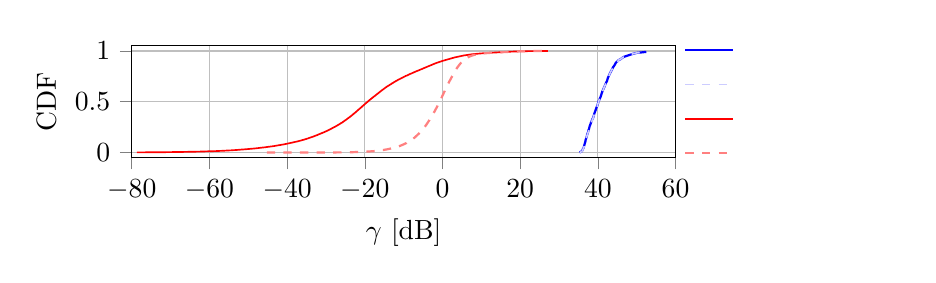
\begin{tikzpicture}

\begin{axis}[
width=0.7\columnwidth,
height=3cm,
legend cell align={left},
legend style={  
  at={(1,0.5)},
  anchor=west,  
  fill opacity=0,
  draw=none,
},
tick align=outside,
tick pos=left,
xlabel={\(\displaystyle \gamma\) [dB]},
xmajorgrids,
xmin=-80, xmax=60,
% xtick={-150,-125,-100,-75,-50,-25,0,25,50,75},
% xticklabels={
%   \(\displaystyle {\ensuremath{-}150}\),
%   \(\displaystyle {\ensuremath{-}125}\),
%   \(\displaystyle {\ensuremath{-}100}\),
%   \(\displaystyle {\ensuremath{-}75}\),
%   \(\displaystyle {\ensuremath{-}50}\),
%   \(\displaystyle {\ensuremath{-}25}\),
%   \(\displaystyle {0}\),
%   \(\displaystyle {25}\),
%   \(\displaystyle {50}\),
%   \(\displaystyle {75}\)
% },
ylabel={CDF},
ymajorgrids,
ymin=-0.0499558823529412, ymax=1.04972058823529,
]
\addplot [thick, blue]
table {%
35.2756147321465 0.001
35.8100215486401 0.011
36.0242817973513 0.021
36.1157180855875 0.031
36.2577350135749 0.041
36.3784510542832 0.051
36.4328553114288 0.061
36.4957888991941 0.071
36.5827678104201 0.081
36.6369275979013 0.091
36.7501785152747 0.101
36.7986680509374 0.111
36.8363762069744 0.121
36.9057648886853 0.131
37.0176018249211 0.141
37.0993870992379 0.151
37.1744455333308 0.161
37.2034207703487 0.171
37.2932923865288 0.181
37.3803810220931 0.191
37.4841631221233 0.201
37.5328909419896 0.211
37.5974033340274 0.221
37.7018321319161 0.231
37.7738702550592 0.241
37.8342046485525 0.251
37.9074116171099 0.261
38.0052193777674 0.271
38.1125939088364 0.281
38.1932974425638 0.291
38.3049359711277 0.301
38.4143564824277 0.311
38.5106963827899 0.321
38.613232928627 0.331
38.7814169284809 0.341
38.8533659435033 0.351
38.9288627471411 0.361
39.0095224296384 0.371
39.0755815853116 0.381
39.1653766820844 0.391
39.2593331213955 0.401
39.3656366012233 0.411
39.4564858466273 0.421
39.5251013308863 0.431
39.6405959193546 0.441
39.7351960015574 0.451
39.8807974178039 0.461
39.9434958101271 0.471
40.0109675249858 0.481
40.0935049304478 0.491
40.1626378518038 0.501
40.2605412700821 0.511
40.3929316795352 0.521
40.490908278938 0.531
40.6256437858775 0.541
40.7283275902067 0.551
40.8225125308664 0.561
40.9132091784675 0.571
40.9639181179053 0.581
41.0722782820416 0.591
41.1520818593127 0.601
41.2769315420947 0.611
41.3747496599138 0.621
41.4933704969212 0.631
41.6145279887043 0.641
41.7378575868063 0.651
41.8213700513768 0.661
41.9319671616491 0.671
42.0474624380567 0.681
42.1425608819456 0.691
42.3386926976943 0.701
42.3909858357034 0.711
42.4835004915664 0.721
42.5469754590876 0.731
42.6571786205682 0.741
42.7754728206726 0.751
42.8891814273974 0.761
43.0108583892235 0.771
43.1210696898258 0.781
43.278184922067 0.791
43.3841674126169 0.801
43.5741274674784 0.811
43.6827232413002 0.821
43.7862530987944 0.831
43.9384225602513 0.841
44.1298261333287 0.851
44.3051486827838 0.861
44.4500473098256 0.871
44.5863127746225 0.881
44.8000251286368 0.891
45.1390196372471 0.901
45.3798727230129 0.911
45.8996435106228 0.921
46.2546401485295 0.931
46.6278242833313 0.941
47.3825137742152 0.951
48.1563467130808 0.961
48.939459425623 0.971
49.9599677179237 0.981
52.4761994188409 0.991
};
\addlegendentry{OPT-CE: $\gamma\oce$}
\addplot [semithick, blue!20!white, dashed]
table {%
35.3502098753063 0.001
35.8649424514539 0.011
36.0978756766435 0.021
36.1478742803768 0.031
36.3046432284919 0.041
36.4020622556272 0.051
36.4835539372502 0.061
36.555609222501 0.071
36.6361180052872 0.081
36.6881081205737 0.091
36.7567687749503 0.101
36.8437839615616 0.111
36.8974375995318 0.121
36.9602972513285 0.131
37.0051571252066 0.141
37.1042017446674 0.151
37.1655158238492 0.161
37.2414400220352 0.171
37.3182764382401 0.181
37.4130873158928 0.191
37.5283546442779 0.201
37.5877695804408 0.211
37.6457889254388 0.221
37.7212851131986 0.231
37.7908115822816 0.241
37.8568712372999 0.251
37.9438824735323 0.261
38.0154692774274 0.271
38.119843328635 0.281
38.2102106719493 0.291
38.3723052845907 0.301
38.5039276429102 0.311
38.5482298662945 0.321
38.6576692740382 0.331
38.8170278697138 0.341
38.8665254110588 0.351
38.9653779077411 0.361
39.0344032465509 0.371
39.0980881294489 0.381
39.1921274995803 0.391
39.2756232505377 0.401
39.4008949358127 0.411
39.4913458280906 0.421
39.5603251999029 0.431
39.6651144312269 0.441
39.7716596827755 0.451
39.8832011228678 0.461
39.9566580382133 0.471
40.0080764083464 0.481
40.1106510934245 0.491
40.196207023207 0.501
40.2707941545521 0.511
40.3592772994345 0.521
40.4938372289383 0.531
40.6367608726525 0.541
40.7328180214447 0.551
40.8482761643324 0.561
40.9403231363995 0.571
40.9813400371335 0.581
41.0921677984393 0.591
41.1717229820326 0.601
41.3050797395016 0.611
41.424440130176 0.621
41.5014647306354 0.631
41.6084443679503 0.641
41.7185439341268 0.651
41.8425404053407 0.661
41.9478902509651 0.671
42.0718212584459 0.681
42.2112515705398 0.691
42.3563423423511 0.701
42.4164350975555 0.711
42.4981897953897 0.721
42.5761352181772 0.731
42.6588825513796 0.741
42.7962381657706 0.751
42.9166431788285 0.761
43.0253409684536 0.771
43.1480214707041 0.781
43.2742038382369 0.791
43.399181088018 0.801
43.557680995483 0.811
43.693888003101 0.821
43.7658351756241 0.831
43.9759117387756 0.841
44.1275201144921 0.851
44.3201341847244 0.861
44.4620812253808 0.871
44.573393114312 0.881
44.8013409045183 0.891
45.2168943660401 0.901
45.3874131683393 0.911
45.9214652652465 0.921
46.2474187369222 0.931
46.6368533780241 0.941
47.3972138830799 0.951
48.1588408085159 0.961
48.9191320832023 0.971
49.9606961004179 0.981
52.4874859960015 0.991
};
\addlegendentry{OPT-CE: $\hat{\gamma}\oce$}
\addplot [semithick, red]
table {%
% -116.606787182071 2.94117647058824e-05
% -91.6000910974723 0.000323529411764706
% -82.8334639018703 0.000617647058823529
% -80.8720260520299 0.000911764705882353
% -79.7279644903591 0.00120588235294118
-78.6888288056727 0.0015
-77.7961434960096 0.00179411764705882
-76.7888379306083 0.00208823529411765
-75.2601143922402 0.00238235294117647
-74.3553084917756 0.00267647058823529
-73.9572811668911 0.00297058823529412
-72.9829954393382 0.00326470588235294
-71.5546684400377 0.00355882352941176
-70.9995784900567 0.00385294117647059
-70.4794471499499 0.00414705882352941
-69.7572503485164 0.00444117647058824
-69.5232204732887 0.00473529411764706
-68.8916413485809 0.00502941176470588
-68.0126816262604 0.00532352941176471
-67.4703927893767 0.00561764705882353
-67.0613450325108 0.00591176470588235
-66.5929072863148 0.00620588235294118
-66.1024211085588 0.0065
-65.9099097076921 0.00679411764705882
-65.6072452130299 0.00708823529411765
-65.0981427266856 0.00738235294117647
-64.8563990032766 0.00767647058823529
-64.2881282797502 0.00797058823529412
-63.8915203373647 0.00826470588235294
-63.5068583405825 0.00855882352941176
-63.2040814872707 0.00885294117647059
-62.7993369949678 0.00914705882352941
-62.4960967194768 0.00944117647058824
-62.2259071660947 0.00973529411764706
-62.0714740297428 0.0100294117647059
-61.7194277487877 0.0103235294117647
-61.5079587903634 0.0106176470588235
-61.2098409528152 0.0109117647058824
-61.0729411054084 0.0112058823529412
-60.8056157013335 0.0115
-60.6249901628488 0.0117941176470588
-60.3905583597867 0.0120882352941176
-59.9284948041879 0.0123823529411765
-59.7048598480941 0.0126764705882353
-59.5159995377754 0.0129705882352941
-59.2224334212442 0.0132647058823529
-58.9676319841606 0.0135588235294118
-58.7316672111895 0.0138529411764706
-58.4930862041693 0.0141470588235294
-58.273121704176 0.0144411764705882
-58.123277297653 0.0147352941176471
-57.9822754704389 0.0150294117647059
-57.7146312294293 0.0153235294117647
-57.5654752505242 0.0156176470588235
-57.4620582071009 0.0159117647058824
-57.2399301427145 0.0162058823529412
-57.0063795014354 0.0165
-56.9138935438746 0.0167941176470588
-56.7821051311324 0.0170882352941176
-56.6847127457201 0.0173823529411765
-56.419877777594 0.0176764705882353
-56.2447297104074 0.0179705882352941
-56.1281679599848 0.0182647058823529
-56.0334280534802 0.0185588235294118
-55.9394359378567 0.0188529411764706
-55.8221383372492 0.0191470588235294
-55.6671647411157 0.0194411764705882
-55.5502672434864 0.0197352941176471
-55.4392824606858 0.0200294117647059
-55.2206465956902 0.0203235294117647
-55.1035969960658 0.0206176470588235
-54.9260979152265 0.0209117647058824
-54.7609314014547 0.0212058823529412
-54.6851172037835 0.0215
-54.4347262322789 0.0217941176470588
-54.3416263461545 0.0220882352941176
-54.2532714910389 0.0223823529411765
-54.130779955661 0.0226764705882353
-53.999715057114 0.0229705882352941
-53.9021315338387 0.0232647058823529
-53.7578686075603 0.0235588235294118
-53.6596949276078 0.0238529411764706
-53.5279694498174 0.0241470588235294
-53.3888512813614 0.0244411764705882
-53.2790745432745 0.0247352941176471
-53.1590449382216 0.0250294117647059
-53.0885762035557 0.0253235294117647
-52.9347108949625 0.0256176470588235
-52.823905445967 0.0259117647058824
-52.7228768047521 0.0262058823529412
-52.6589081616874 0.0265
-52.5334588704915 0.0267941176470588
-52.396753678046 0.0270882352941176
-52.2663005449583 0.0273823529411765
-52.2044521041436 0.0276764705882353
-52.136781002182 0.0279705882352941
-52.0626442564152 0.0282647058823529
-51.9878145387623 0.0285588235294118
-51.9432427512115 0.0288529411764706
-51.8598333043369 0.0291470588235294
-51.7553846037918 0.0294411764705882
-51.6452757135348 0.0297352941176471
-51.5739615042912 0.0300294117647059
-51.4454679576108 0.0303235294117647
-51.3081914117541 0.0306176470588235
-51.1452490574473 0.0309117647058824
-51.0322045288424 0.0312058823529412
-50.958450368026 0.0315
-50.8681508654108 0.0317941176470588
-50.7361549195916 0.0320882352941176
-50.6986655569937 0.0323823529411765
-50.6094887325036 0.0326764705882353
-50.507654614468 0.0329705882352941
-50.4158718926678 0.0332647058823529
-50.3199396215424 0.0335588235294118
-50.2564078934873 0.0338529411764706
-50.1808927404638 0.0341470588235294
-50.0382366412612 0.0344411764705882
-49.9749379925647 0.0347352941176471
-49.9008591887096 0.0350294117647059
-49.8397127003919 0.0353235294117647
-49.7216055685861 0.0356176470588235
-49.6943114819245 0.0359117647058824
-49.6318470691724 0.0362058823529412
-49.4827510346049 0.0365
-49.4251740789995 0.0367941176470588
-49.2816296662181 0.0370882352941176
-49.1703692645909 0.0373823529411765
-49.0871415729302 0.0376764705882353
-48.9846013926524 0.0379705882352941
-48.9346656320675 0.0382647058823529
-48.8287720123447 0.0385588235294118
-48.7157276236608 0.0388529411764706
-48.6600199794699 0.0391470588235294
-48.5915267565477 0.0394411764705882
-48.5043841340782 0.0397352941176471
-48.4008387644487 0.0400294117647059
-48.3219041527521 0.0403235294117647
-48.2645024392311 0.0406176470588235
-48.1795301982119 0.0409117647058824
-48.0926721604291 0.0412058823529412
-48.0468529395755 0.0415
-47.9692965452668 0.0417941176470588
-47.8684514594831 0.0420882352941176
-47.8088154366407 0.0423823529411765
-47.7563624856973 0.0426764705882353
-47.7080113956058 0.0429705882352941
-47.6444039700816 0.0432647058823529
-47.5927776611867 0.0435588235294118
-47.517326756589 0.0438529411764706
-47.4489362453069 0.0441470588235294
-47.3921863853668 0.0444411764705882
-47.29622280857 0.0447352941176471
-47.2517415100318 0.0450294117647059
-47.1834725687228 0.0453235294117647
-47.1497467640561 0.0456176470588235
-47.0671194775589 0.0459117647058824
-47.01322295436 0.0462058823529412
-46.945398963561 0.0465
-46.8650738739553 0.0467941176470588
-46.8043010022853 0.0470882352941176
-46.7299487228219 0.0473823529411765
-46.6562216792953 0.0476764705882353
-46.5964883371812 0.0479705882352941
-46.5413093123991 0.0482647058823529
-46.4808170104259 0.0485588235294118
-46.435341909205 0.0488529411764706
-46.3830429868089 0.0491470588235294
-46.3025523769489 0.0494411764705882
-46.187048087475 0.0497352941176471
-46.1153400509618 0.0500294117647059
-46.0410848883137 0.0503235294117647
-45.9494234391797 0.0506176470588235
-45.8871553155385 0.0509117647058824
-45.8352286181784 0.0512058823529412
-45.7747125918398 0.0515
-45.7092009437694 0.0517941176470588
-45.6691435755472 0.0520882352941177
-45.6057900832189 0.0523823529411765
-45.5473947924024 0.0526764705882353
-45.5068539090182 0.0529705882352941
-45.4348346968909 0.0532647058823529
-45.3735109069257 0.0535588235294118
-45.3313091603651 0.0538529411764706
-45.2562363132508 0.0541470588235294
-45.2133564652213 0.0544411764705882
-45.1750311746556 0.0547352941176471
-45.1243690995562 0.0550294117647059
-45.0733643392849 0.0553235294117647
-45.0076408245156 0.0556176470588235
-44.9604924896654 0.0559117647058824
-44.8901755580778 0.0562058823529412
-44.8255384882825 0.0565
-44.7761165091973 0.0567941176470588
-44.7188448205253 0.0570882352941176
-44.625656964665 0.0573823529411765
-44.5823599256198 0.0576764705882353
-44.5252433179865 0.0579705882352941
-44.4646975184233 0.0582647058823529
-44.4229771561171 0.0585588235294118
-44.3588136955211 0.0588529411764706
-44.2731938241197 0.0591470588235294
-44.2182217328878 0.0594411764705882
-44.1704117317405 0.0597352941176471
-44.1280942869549 0.0600294117647059
-44.0454879927002 0.0603235294117647
-43.9978204017756 0.0606176470588235
-43.934296296073 0.0609117647058824
-43.8651170616148 0.0612058823529412
-43.8014053402376 0.0615
-43.7509507995421 0.0617941176470588
-43.6991942042057 0.0620882352941176
-43.6594895922561 0.0623823529411765
-43.6057843588407 0.0626764705882353
-43.5673053739955 0.0629705882352941
-43.5005236673591 0.0632647058823529
-43.4358264869028 0.0635588235294118
-43.3981057425968 0.0638529411764706
-43.3557937792587 0.0641470588235294
-43.2905950788833 0.0644411764705882
-43.2349731975821 0.0647352941176471
-43.1891995946253 0.0650294117647059
-43.148621697619 0.0653235294117647
-43.1244222343644 0.0656176470588235
-43.0584914800404 0.0659117647058824
-42.9911917842791 0.0662058823529412
-42.9689191387906 0.0665
-42.9195193814141 0.0667941176470588
-42.8870042768711 0.0670882352941176
-42.8273725849287 0.0673823529411765
-42.7911544426173 0.0676764705882353
-42.7522951173142 0.0679705882352941
-42.7114228419027 0.0682647058823529
-42.6811559243483 0.0685588235294118
-42.6333231707568 0.0688529411764706
-42.5976847744937 0.0691470588235294
-42.5464685023158 0.0694411764705882
-42.4970175166543 0.0697352941176471
-42.4655312826779 0.0700294117647059
-42.4226228654366 0.0703235294117647
-42.3581155246162 0.0706176470588235
-42.308612185712 0.0709117647058824
-42.2704182328131 0.0712058823529412
-42.2169734720793 0.0715
-42.170306257262 0.0717941176470588
-42.1267362216948 0.0720882352941176
-42.0760378632601 0.0723823529411765
-42.0290505694395 0.0726764705882353
-41.988034155105 0.0729705882352941
-41.9398031795562 0.0732647058823529
-41.8812017760201 0.0735588235294118
-41.8230198630257 0.0738529411764706
-41.7816317724641 0.0741470588235294
-41.7407850023714 0.0744411764705882
-41.6924456442383 0.0747352941176471
-41.6748772521536 0.0750294117647059
-41.64193660071 0.0753235294117647
-41.6014692713015 0.0756176470588235
-41.564414865647 0.0759117647058824
-41.5364211272879 0.0762058823529412
-41.4913702727462 0.0765
-41.4424850407499 0.0767941176470588
-41.3975975827265 0.0770882352941177
-41.3424559917306 0.0773823529411765
-41.3124889113533 0.0776764705882353
-41.2672970998302 0.0779705882352941
-41.1928812598014 0.0782647058823529
-41.1485551234716 0.0785588235294118
-41.0975888357809 0.0788529411764706
-41.0666457255288 0.0791470588235294
-41.0111366564519 0.0794411764705882
-40.9810973965189 0.0797352941176471
-40.9373128774339 0.0800294117647059
-40.9019822461572 0.0803235294117647
-40.8583144187497 0.0806176470588235
-40.820975741732 0.0809117647058823
-40.7713031231097 0.0812058823529412
-40.7385910912793 0.0815
-40.701203355324 0.0817941176470588
-40.6746806211639 0.0820882352941176
-40.63840828416 0.0823823529411765
-40.6041107211624 0.0826764705882353
-40.5615892296864 0.0829705882352941
-40.4983371923856 0.0832647058823529
-40.4498077225703 0.0835588235294118
-40.4157952822273 0.0838529411764706
-40.3868093428795 0.0841470588235294
-40.3507106852464 0.0844411764705882
-40.3087470261792 0.0847352941176471
-40.2654876441142 0.0850294117647059
-40.2435815358026 0.0853235294117647
-40.1925611854984 0.0856176470588235
-40.1544597250666 0.0859117647058824
-40.1024446421071 0.0862058823529412
-40.0756422739768 0.0865
-40.0419987874005 0.0867941176470588
-40.0087247477996 0.0870882352941176
-39.964612726213 0.0873823529411765
-39.9403016612422 0.0876764705882353
-39.8946174056551 0.0879705882352941
-39.8580556349935 0.0882647058823529
-39.8299041391886 0.0885588235294118
-39.8021049434479 0.0888529411764706
-39.7766803857232 0.0891470588235294
-39.7458330101755 0.0894411764705882
-39.7188784316827 0.0897352941176471
-39.6783860760635 0.0900294117647059
-39.6381586317399 0.0903235294117647
-39.6097119385189 0.0906176470588235
-39.5595960565536 0.0909117647058824
-39.5244580280329 0.0912058823529412
-39.4878382000955 0.0915
-39.4630618616125 0.0917941176470588
-39.4290381610347 0.0920882352941177
-39.4029359674463 0.0923823529411765
-39.3532324302877 0.0926764705882353
-39.3249927506788 0.0929705882352941
-39.2812461248385 0.0932647058823529
-39.2408764844749 0.0935588235294118
-39.2070618570656 0.0938529411764706
-39.1841697852375 0.0941470588235294
-39.1550616724043 0.0944411764705882
-39.1301740720068 0.0947352941176471
-39.0892455878663 0.0950294117647059
-39.0444162674211 0.0953235294117647
-39.0126773697713 0.0956176470588235
-38.97618955789 0.0959117647058823
-38.9436917692111 0.0962058823529412
-38.8886818511319 0.0965
-38.8470479063756 0.0967941176470588
-38.7831001165975 0.0970882352941176
-38.7614782278384 0.0973823529411765
-38.7298048279399 0.0976764705882353
-38.6790749512532 0.0979705882352941
-38.6506194503907 0.0982647058823529
-38.6113158679972 0.0985588235294118
-38.5766835488017 0.0988529411764706
-38.5372106887054 0.0991470588235294
-38.4966448322791 0.0994411764705882
-38.4798641221178 0.0997352941176471
-38.4655330214574 0.100029411764706
-38.4175797921589 0.100323529411765
-38.3937072251878 0.100617647058824
-38.3729054193203 0.100911764705882
-38.3343361931632 0.101205882352941
-38.3029439842526 0.1015
-38.2443793988884 0.101794117647059
-38.2233440369115 0.102088235294118
-38.1851405381434 0.102382352941176
-38.1627736552255 0.102676470588235
-38.1184204206939 0.102970588235294
-38.092564171003 0.103264705882353
-38.0683688242794 0.103558823529412
-38.0212746999547 0.103852941176471
-37.9937311882991 0.104147058823529
-37.9766360861855 0.104441176470588
-37.9429405396698 0.104735294117647
-37.9123659133669 0.105029411764706
-37.87054689157 0.105323529411765
-37.806733010471 0.105617647058824
-37.7625069151217 0.105911764705882
-37.7324544061991 0.106205882352941
-37.7110007419323 0.1065
-37.6623938463691 0.106794117647059
-37.6216730594367 0.107088235294118
-37.5840803711894 0.107382352941176
-37.5588009381078 0.107676470588235
-37.5266212058758 0.107970588235294
-37.4971606768703 0.108264705882353
-37.4576189224411 0.108558823529412
-37.4241685398166 0.108852941176471
-37.3943194383718 0.109147058823529
-37.3796044582317 0.109441176470588
-37.339674305801 0.109735294117647
-37.3042360563432 0.110029411764706
-37.2722023807265 0.110323529411765
-37.2449779353726 0.110617647058824
-37.2270416968419 0.110911764705882
-37.1957756894616 0.111205882352941
-37.1577586079028 0.1115
-37.1216371801469 0.111794117647059
-37.0767225327898 0.112088235294118
-37.0395237143506 0.112382352941176
-37.0078584738784 0.112676470588235
-36.9834671105388 0.112970588235294
-36.9631735700666 0.113264705882353
-36.9345846450532 0.113558823529412
-36.9188220551857 0.113852941176471
-36.887305438342 0.114147058823529
-36.854099698454 0.114441176470588
-36.826047780575 0.114735294117647
-36.8007014906934 0.115029411764706
-36.7550983109351 0.115323529411765
-36.741354760173 0.115617647058824
-36.7177661833501 0.115911764705882
-36.6915469704838 0.116205882352941
-36.6615847966274 0.1165
-36.6263951489531 0.116794117647059
-36.5819333012811 0.117088235294118
-36.5603271294377 0.117382352941176
-36.5236897720011 0.117676470588235
-36.5038085847437 0.117970588235294
-36.4854676290247 0.118264705882353
-36.4648077382338 0.118558823529412
-36.4386174958549 0.118852941176471
-36.4203674927825 0.119147058823529
-36.3974140660405 0.119441176470588
-36.3780001298288 0.119735294117647
-36.3345693394573 0.120029411764706
-36.3085428551588 0.120323529411765
-36.2825838586011 0.120617647058824
-36.2590953811829 0.120911764705882
-36.232458301523 0.121205882352941
-36.2051841641452 0.1215
-36.1623277159447 0.121794117647059
-36.1445994644638 0.122088235294118
-36.1096956489245 0.122382352941176
-36.0916676935194 0.122676470588235
-36.0603714823606 0.122970588235294
-36.0325831656524 0.123264705882353
-35.9931277985071 0.123558823529412
-35.9556498192589 0.123852941176471
-35.9263799218886 0.124147058823529
-35.9000067472768 0.124441176470588
-35.8671022502407 0.124735294117647
-35.831179059286 0.125029411764706
-35.8129716506128 0.125323529411765
-35.7922728234645 0.125617647058824
-35.7684967514123 0.125911764705882
-35.7298411087402 0.126205882352941
-35.7087312964004 0.1265
-35.6500858601006 0.126794117647059
-35.6265451418538 0.127088235294118
-35.6108878131606 0.127382352941176
-35.5964087387838 0.127676470588235
-35.5815454829114 0.127970588235294
-35.5473811238212 0.128264705882353
-35.5289331555084 0.128558823529412
-35.5064282960065 0.128852941176471
-35.4891226205216 0.129147058823529
-35.4712094082742 0.129441176470588
-35.4477347456722 0.129735294117647
-35.4274840806393 0.130029411764706
-35.3928564633992 0.130323529411765
-35.3696769897609 0.130617647058824
-35.3309916331661 0.130911764705882
-35.3088501647119 0.131205882352941
-35.2808584712122 0.1315
-35.2609363144648 0.131794117647059
-35.2425620789586 0.132088235294118
-35.2069694640676 0.132382352941176
-35.1787282113 0.132676470588235
-35.1473753187989 0.132970588235294
-35.1235187497805 0.133264705882353
-35.1071642144417 0.133558823529412
-35.06908281716 0.133852941176471
-35.0489960490701 0.134147058823529
-35.0278861859124 0.134441176470588
-35.0125226672716 0.134735294117647
-34.9989340277421 0.135029411764706
-34.9717572063292 0.135323529411765
-34.9571980820026 0.135617647058824
-34.9279530603064 0.135911764705882
-34.8938225558058 0.136205882352941
-34.8682791441206 0.1365
-34.8345374914794 0.136794117647059
-34.797300546572 0.137088235294118
-34.7817361801669 0.137382352941176
-34.7428900671592 0.137676470588235
-34.7164557517157 0.137970588235294
-34.6899234074781 0.138264705882353
-34.6808168810473 0.138558823529412
-34.658568227239 0.138852941176471
-34.6338693583579 0.139147058823529
-34.6205439367147 0.139441176470588
-34.6014999028412 0.139735294117647
-34.5773650085268 0.140029411764706
-34.5586262495564 0.140323529411765
-34.5363119600509 0.140617647058824
-34.5198569296972 0.140911764705882
-34.4992854350017 0.141205882352941
-34.4757900966885 0.1415
-34.4591800877504 0.141794117647059
-34.4370467090548 0.142088235294118
-34.4009196996677 0.142382352941176
-34.374818065549 0.142676470588235
-34.3591492595655 0.142970588235294
-34.341421925498 0.143264705882353
-34.3246377876068 0.143558823529412
-34.2994952632843 0.143852941176471
-34.2713576490134 0.144147058823529
-34.2558161698623 0.144441176470588
-34.24606479496 0.144735294117647
-34.2256158035974 0.145029411764706
-34.1994092019993 0.145323529411765
-34.187762954464 0.145617647058824
-34.1549041853148 0.145911764705882
-34.1260715780792 0.146205882352941
-34.1057796988611 0.1465
-34.0829902785825 0.146794117647059
-34.0459137683823 0.147088235294118
-34.0307692860233 0.147382352941176
-34.0086686191959 0.147676470588235
-33.9938325891108 0.147970588235294
-33.964598762059 0.148264705882353
-33.9408625189984 0.148558823529412
-33.898325725828 0.148852941176471
-33.8745889445772 0.149147058823529
-33.8503736647874 0.149441176470588
-33.8207652846792 0.149735294117647
-33.8014106009075 0.150029411764706
-33.7844953414703 0.150323529411765
-33.7680308024146 0.150617647058824
-33.7508089451779 0.150911764705882
-33.7301587773022 0.151205882352941
-33.7149426854676 0.1515
-33.6966226195067 0.151794117647059
-33.6816261427067 0.152088235294118
-33.6622788501505 0.152382352941176
-33.6274108191052 0.152676470588235
-33.5934445505538 0.152970588235294
-33.5736810647188 0.153264705882353
-33.5463966785647 0.153558823529412
-33.5211171188552 0.153852941176471
-33.497213864098 0.154147058823529
-33.4862982451887 0.154441176470588
-33.4777394141681 0.154735294117647
-33.4527554954029 0.155029411764706
-33.4372784645178 0.155323529411765
-33.4097014652895 0.155617647058824
-33.3967297560398 0.155911764705882
-33.3667620724353 0.156205882352941
-33.3409825753658 0.1565
-33.3159072611767 0.156794117647059
-33.2878096547924 0.157088235294118
-33.2681370935156 0.157382352941176
-33.2589448660743 0.157676470588235
-33.2377100437494 0.157970588235294
-33.2183359614429 0.158264705882353
-33.2091570083906 0.158558823529412
-33.1646751727185 0.158852941176471
-33.1509452313182 0.159147058823529
-33.128520874535 0.159441176470588
-33.1107892118151 0.159735294117647
-33.0872192307462 0.160029411764706
-33.0713579923329 0.160323529411765
-33.0393097217708 0.160617647058824
-33.0269084381339 0.160911764705882
-33.0056880830846 0.161205882352941
-32.9835026245333 0.1615
-32.9625129659722 0.161794117647059
-32.9384536499503 0.162088235294118
-32.9136897181154 0.162382352941176
-32.9007758278412 0.162676470588235
-32.8921642263296 0.162970588235294
-32.8788995065205 0.163264705882353
-32.849649777316 0.163558823529412
-32.8288944520853 0.163852941176471
-32.8085810302243 0.164147058823529
-32.7870408760852 0.164441176470588
-32.7706431126876 0.164735294117647
-32.7522528373915 0.165029411764706
-32.7366028316938 0.165323529411765
-32.7217070656353 0.165617647058824
-32.6967424899024 0.165911764705882
-32.6815158139391 0.166205882352941
-32.6479500817315 0.1665
-32.6379198763687 0.166794117647059
-32.6085519870071 0.167088235294118
-32.5912472227798 0.167382352941176
-32.5711841261946 0.167676470588235
-32.5532620434043 0.167970588235294
-32.5322261129178 0.168264705882353
-32.5140732100651 0.168558823529412
-32.4986793074734 0.168852941176471
-32.4815994330548 0.169147058823529
-32.4641001669104 0.169441176470588
-32.4363782129147 0.169735294117647
-32.4151796749225 0.170029411764706
-32.3959689137384 0.170323529411765
-32.379233467902 0.170617647058824
-32.3408887253137 0.170911764705882
-32.3265076599532 0.171205882352941
-32.3020794865749 0.1715
-32.2796627364644 0.171794117647059
-32.2613453488597 0.172088235294118
-32.2425571192933 0.172382352941176
-32.2190000022007 0.172676470588235
-32.2118280205332 0.172970588235294
-32.2021282461059 0.173264705882353
-32.1866659792518 0.173558823529412
-32.1689927610304 0.173852941176471
-32.1563879793192 0.174147058823529
-32.143077181293 0.174441176470588
-32.1167950662828 0.174735294117647
-32.0999557505603 0.175029411764706
-32.0772845160491 0.175323529411765
-32.0604463889311 0.175617647058824
-32.0332919254662 0.175911764705882
-32.0031388308064 0.176205882352941
-31.9887601348014 0.1765
-31.9720452463302 0.176794117647059
-31.9635462845391 0.177088235294118
-31.9457719660492 0.177382352941176
-31.9299636735942 0.177676470588235
-31.9081941349255 0.177970588235294
-31.8876376989956 0.178264705882353
-31.8708794953378 0.178558823529412
-31.8512951573215 0.178852941176471
-31.8322338300694 0.179147058823529
-31.8170549246494 0.179441176470588
-31.8063237580924 0.179735294117647
-31.7884539628195 0.180029411764706
-31.7618883562306 0.180323529411765
-31.7427750973424 0.180617647058824
-31.7278518289901 0.180911764705882
-31.7133842451573 0.181205882352941
-31.6861924917711 0.1815
-31.6586162859347 0.181794117647059
-31.6341735706097 0.182088235294118
-31.6159340889587 0.182382352941176
-31.5987988842665 0.182676470588235
-31.5792084192995 0.182970588235294
-31.5729157494867 0.183264705882353
-31.5617104465508 0.183558823529412
-31.5489157785704 0.183852941176471
-31.5299980254108 0.184147058823529
-31.5111156381454 0.184441176470588
-31.4927163247991 0.184735294117647
-31.4789011053823 0.185029411764706
-31.4634822250816 0.185323529411765
-31.4474084369513 0.185617647058824
-31.425799726611 0.185911764705882
-31.3984835145186 0.186205882352941
-31.3857093812376 0.1865
-31.371443591607 0.186794117647059
-31.3529723616673 0.187088235294118
-31.3362478945227 0.187382352941176
-31.3241349398512 0.187676470588235
-31.3044431846659 0.187970588235294
-31.2791430900421 0.188264705882353
-31.2630652876934 0.188558823529412
-31.2374594322596 0.188852941176471
-31.2274206683331 0.189147058823529
-31.2137020859596 0.189441176470588
-31.1909747986341 0.189735294117647
-31.158483412523 0.190029411764706
-31.1491714410067 0.190323529411765
-31.1207738216053 0.190617647058824
-31.10328866093 0.190911764705882
-31.0880620110762 0.191205882352941
-31.0534505973909 0.1915
-31.0316899622344 0.191794117647059
-31.0042452788182 0.192088235294118
-30.9854336693059 0.192382352941176
-30.976867982612 0.192676470588235
-30.9485958495864 0.192970588235294
-30.9279250126427 0.193264705882353
-30.9103794568402 0.193558823529412
-30.8922869033223 0.193852941176471
-30.8776554294247 0.194147058823529
-30.8649811125515 0.194441176470588
-30.8435458651602 0.194735294117647
-30.8196699407945 0.195029411764706
-30.8076613014686 0.195323529411765
-30.7886231817308 0.195617647058824
-30.7704681959079 0.195911764705882
-30.7567588703287 0.196205882352941
-30.7399012067567 0.1965
-30.7261367067771 0.196794117647059
-30.7021913577189 0.197088235294118
-30.688717777671 0.197382352941176
-30.6667025414352 0.197676470588235
-30.648572685574 0.197970588235294
-30.627748524041 0.198264705882353
-30.6047118157451 0.198558823529412
-30.5880632543846 0.198852941176471
-30.5690689399359 0.199147058823529
-30.5555830364749 0.199441176470588
-30.5279484667952 0.199735294117647
-30.508446954359 0.200029411764706
-30.4875882002178 0.200323529411765
-30.4760535156037 0.200617647058824
-30.454382416263 0.200911764705882
-30.4412165489068 0.201205882352941
-30.4213045141641 0.2015
-30.396026804075 0.201794117647059
-30.3809817925481 0.202088235294118
-30.3640699565705 0.202382352941176
-30.3490069758633 0.202676470588235
-30.3299209547106 0.202970588235294
-30.3136381224169 0.203264705882353
-30.3042503206833 0.203558823529412
-30.287894141352 0.203852941176471
-30.2668433428162 0.204147058823529
-30.246804556424 0.204441176470588
-30.2290391655797 0.204735294117647
-30.2121907450904 0.205029411764706
-30.2025273669294 0.205323529411765
-30.1822923516957 0.205617647058824
-30.1582943988197 0.205911764705882
-30.1467295149752 0.206205882352941
-30.1312707005926 0.2065
-30.1194535404139 0.206794117647059
-30.1014624311093 0.207088235294118
-30.0865240588263 0.207382352941176
-30.0718408374267 0.207676470588235
-30.057497998671 0.207970588235294
-30.030823659199 0.208264705882353
-30.0083290481181 0.208558823529412
-29.9852478583532 0.208852941176471
-29.9731186262387 0.209147058823529
-29.9617251720851 0.209441176470588
-29.9409064796546 0.209735294117647
-29.9230214462807 0.210029411764706
-29.9116536946401 0.210323529411765
-29.8841615732751 0.210617647058824
-29.8618772725321 0.210911764705882
-29.8378607118775 0.211205882352941
-29.8123448875802 0.2115
-29.8010344309204 0.211794117647059
-29.7898880166494 0.212088235294118
-29.7779863861988 0.212382352941176
-29.7593554276254 0.212676470588235
-29.7460938540474 0.212970588235294
-29.7357835196269 0.213264705882353
-29.7212729614099 0.213558823529412
-29.7033108176579 0.213852941176471
-29.6934288051929 0.214147058823529
-29.6849441475521 0.214441176470588
-29.6626981214206 0.214735294117647
-29.645598137587 0.215029411764706
-29.6351965989791 0.215323529411765
-29.619940173018 0.215617647058824
-29.6052302644267 0.215911764705882
-29.5944576131597 0.216205882352941
-29.5702351052583 0.2165
-29.5496992684697 0.216794117647059
-29.5404803889388 0.217088235294118
-29.5274864565609 0.217382352941176
-29.5171205572028 0.217676470588235
-29.5082509527664 0.217970588235294
-29.4906441364165 0.218264705882353
-29.4707483062596 0.218558823529412
-29.4593066770053 0.218852941176471
-29.4501878859826 0.219147058823529
-29.4377175107235 0.219441176470588
-29.428662466376 0.219735294117647
-29.4161897612433 0.220029411764706
-29.4007359584526 0.220323529411765
-29.3816197706502 0.220617647058824
-29.3676802861053 0.220911764705882
-29.3533419714814 0.221205882352941
-29.3361608669827 0.2215
-29.31679784883 0.221794117647059
-29.2953113865343 0.222088235294118
-29.2771424153605 0.222382352941176
-29.2687313080736 0.222676470588235
-29.253012899551 0.222970588235294
-29.2357745741517 0.223264705882353
-29.2188021344244 0.223558823529412
-29.1892535034597 0.223852941176471
-29.1736614862261 0.224147058823529
-29.1603580431283 0.224441176470588
-29.1427227163261 0.224735294117647
-29.1261807874085 0.225029411764706
-29.1084352362738 0.225323529411765
-29.0908262209329 0.225617647058824
-29.0770347806089 0.225911764705882
-29.0653323485963 0.226205882352941
-29.0490194988824 0.2265
-29.0362179295502 0.226794117647059
-29.020636377609 0.227088235294118
-29.0073979462722 0.227382352941176
-28.9863681694945 0.227676470588235
-28.9767605674637 0.227970588235294
-28.9608864657101 0.228264705882353
-28.9439813103823 0.228558823529412
-28.923587979443 0.228852941176471
-28.911233481159 0.229147058823529
-28.891085002527 0.229441176470588
-28.8746557361947 0.229735294117647
-28.8641325516608 0.230029411764706
-28.85478563862 0.230323529411765
-28.8447246309593 0.230617647058824
-28.8334310948099 0.230911764705882
-28.8224515433173 0.231205882352941
-28.8107609975353 0.2315
-28.7973624865856 0.231794117647059
-28.7730973405451 0.232088235294118
-28.7604085542713 0.232382352941176
-28.7438062599829 0.232676470588235
-28.7259529051381 0.232970588235294
-28.6999379515089 0.233264705882353
-28.6820234838116 0.233558823529412
-28.6704820733682 0.233852941176471
-28.6613503955108 0.234147058823529
-28.6439777634847 0.234441176470588
-28.6284510928823 0.234735294117647
-28.6064520707179 0.235029411764706
-28.5978149738571 0.235323529411765
-28.5833975689547 0.235617647058824
-28.5712009116666 0.235911764705882
-28.5611109512834 0.236205882352941
-28.5491834806334 0.2365
-28.5365860376942 0.236794117647059
-28.5221008254148 0.237088235294118
-28.4978592655968 0.237382352941176
-28.4914261726519 0.237676470588235
-28.4758847514337 0.237970588235294
-28.4639502170761 0.238264705882353
-28.4487151917877 0.238558823529412
-28.4323509173003 0.238852941176471
-28.4149360784134 0.239147058823529
-28.4039753394424 0.239441176470588
-28.3956763160692 0.239735294117647
-28.3758470657901 0.240029411764706
-28.3671212858822 0.240323529411765
-28.3574430532028 0.240617647058824
-28.3439304817889 0.240911764705882
-28.3357646476886 0.241205882352941
-28.3201467566031 0.2415
-28.3006578760391 0.241794117647059
-28.2872471407196 0.242088235294118
-28.2664506566089 0.242382352941176
-28.243839014223 0.242676470588235
-28.2190108353879 0.242970588235294
-28.2056400157153 0.243264705882353
-28.1914247309604 0.243558823529412
-28.1827584194867 0.243852941176471
-28.1677302175678 0.244147058823529
-28.1548108849179 0.244441176470588
-28.1485994596092 0.244735294117647
-28.1443380861991 0.245029411764706
-28.1269266892435 0.245323529411765
-28.1130461980952 0.245617647058824
-28.095662652895 0.245911764705882
-28.0846126138953 0.246205882352941
-28.0715669339112 0.2465
-28.0532904231863 0.246794117647059
-28.0431475272842 0.247088235294118
-28.0254454738754 0.247382352941176
-28.0068412150817 0.247676470588235
-27.9924286013141 0.247970588235294
-27.9770763326824 0.248264705882353
-27.9596059937387 0.248558823529412
-27.9388807172033 0.248852941176471
-27.9265140054386 0.249147058823529
-27.9138022219646 0.249441176470588
-27.9004556202303 0.249735294117647
-27.8883696594033 0.250029411764706
-27.8725618977199 0.250323529411765
-27.8563774919921 0.250617647058824
-27.8298788029267 0.250911764705882
-27.8202388880763 0.251205882352941
-27.8092575408872 0.2515
-27.7953849257285 0.251794117647059
-27.7771551039345 0.252088235294118
-27.763012800049 0.252382352941176
-27.7519260975348 0.252676470588235
-27.736966823579 0.252970588235294
-27.7186976993775 0.253264705882353
-27.7075824519366 0.253558823529412
-27.6993648591138 0.253852941176471
-27.6856770423567 0.254147058823529
-27.676894652363 0.254441176470588
-27.6537748464405 0.254735294117647
-27.6317774728632 0.255029411764706
-27.6129556282648 0.255323529411765
-27.5959189224308 0.255617647058824
-27.5768975325487 0.255911764705882
-27.5687417824317 0.256205882352941
-27.5586719947801 0.2565
-27.5505408100853 0.256794117647059
-27.525079481457 0.257088235294118
-27.5083100127146 0.257382352941176
-27.4901171711245 0.257676470588235
-27.4731672364037 0.257970588235294
-27.4596494655969 0.258264705882353
-27.4501317716629 0.258558823529412
-27.4359754258819 0.258852941176471
-27.4295642595308 0.259147058823529
-27.4141746130671 0.259441176470588
-27.4027640961248 0.259735294117647
-27.3906581415366 0.260029411764706
-27.3822244687133 0.260323529411765
-27.3621340500184 0.260617647058824
-27.3514000403544 0.260911764705882
-27.3363489939805 0.261205882352941
-27.3268883894839 0.2615
-27.3134902185279 0.261794117647059
-27.2985701803467 0.262088235294118
-27.2906024467388 0.262382352941176
-27.2802668659169 0.262676470588235
-27.2697508724921 0.262970588235294
-27.2597346210759 0.263264705882353
-27.2423595731944 0.263558823529412
-27.22409364581 0.263852941176471
-27.2116097304695 0.264147058823529
-27.2011886062842 0.264441176470588
-27.190113989976 0.264735294117647
-27.1794119665882 0.265029411764706
-27.1678310299006 0.265323529411765
-27.1539124315489 0.265617647058824
-27.1361687155743 0.265911764705882
-27.1249771851899 0.266205882352941
-27.1164129066059 0.2665
-27.1052435706431 0.266794117647059
-27.0910933085172 0.267088235294118
-27.0821246120205 0.267382352941176
-27.0626110167734 0.267676470588235
-27.0520332041296 0.267970588235294
-27.0388283186977 0.268264705882353
-27.0262203197636 0.268558823529412
-27.008104305835 0.268852941176471
-26.9915428333397 0.269147058823529
-26.9782522343042 0.269441176470588
-26.9614235636777 0.269735294117647
-26.9482343811813 0.270029411764706
-26.9348838753991 0.270323529411765
-26.9219711315831 0.270617647058824
-26.9096508370916 0.270911764705882
-26.900081906092 0.271205882352941
-26.8872745490858 0.2715
-26.8730523224577 0.271794117647059
-26.8596126193595 0.272088235294118
-26.8377087847664 0.272382352941176
-26.8197839780406 0.272676470588235
-26.8079305678429 0.272970588235294
-26.7938877775992 0.273264705882353
-26.7847059718941 0.273558823529412
-26.7698232555199 0.273852941176471
-26.7576748353373 0.274147058823529
-26.7479332414569 0.274441176470588
-26.7335229722468 0.274735294117647
-26.7140028227343 0.275029411764706
-26.7055354982934 0.275323529411765
-26.6908353925715 0.275617647058824
-26.6792762221331 0.275911764705882
-26.6676793983922 0.276205882352941
-26.6566092739399 0.2765
-26.6466418002484 0.276794117647059
-26.6390037830803 0.277088235294118
-26.6277833690823 0.277382352941176
-26.6206214520116 0.277676470588235
-26.6066919673483 0.277970588235294
-26.5952857875695 0.278264705882353
-26.5866179932293 0.278558823529412
-26.5715171264612 0.278852941176471
-26.5504073861269 0.279147058823529
-26.5400267336298 0.279441176470588
-26.524239311087 0.279735294117647
-26.5139190733339 0.280029411764706
-26.4999001652577 0.280323529411765
-26.4845041361224 0.280617647058824
-26.476868201808 0.280911764705882
-26.4632163020342 0.281205882352941
-26.453976888881 0.2815
-26.4456847175715 0.281794117647059
-26.4300532880641 0.282088235294118
-26.4159650391603 0.282382352941176
-26.4025944375458 0.282676470588235
-26.3885217992454 0.282970588235294
-26.3734041801361 0.283264705882353
-26.3636102261691 0.283558823529412
-26.3558635733914 0.283852941176471
-26.3394898094696 0.284147058823529
-26.321362176321 0.284441176470588
-26.3083269446993 0.284735294117647
-26.3017367145908 0.285029411764706
-26.292900978648 0.285323529411765
-26.2813953143575 0.285617647058824
-26.2708141358871 0.285911764705882
-26.2576369113081 0.286205882352941
-26.2420645633558 0.2865
-26.2303414137054 0.286794117647059
-26.2207890709805 0.287088235294118
-26.2100403734149 0.287382352941176
-26.190089947769 0.287676470588235
-26.1768763293063 0.287970588235294
-26.1626460623904 0.288264705882353
-26.1576895958587 0.288558823529412
-26.1496066820227 0.288852941176471
-26.1328339832681 0.289147058823529
-26.1189768883639 0.289441176470588
-26.1070829654025 0.289735294117647
-26.0984959399415 0.290029411764706
-26.0814649903239 0.290323529411765
-26.0644184929473 0.290617647058824
-26.0515868251399 0.290911764705882
-26.0386675144551 0.291205882352941
-26.0205408650314 0.2915
-25.9954784562924 0.291794117647059
-25.9820181760764 0.292088235294118
-25.9632501195378 0.292382352941176
-25.9526582976025 0.292676470588235
-25.9360615976898 0.292970588235294
-25.9216534143878 0.293264705882353
-25.9089011029105 0.293558823529412
-25.9001358983831 0.293852941176471
-25.8887344145011 0.294147058823529
-25.8777003434979 0.294441176470588
-25.8640397462341 0.294735294117647
-25.8526255267617 0.295029411764706
-25.8397266429989 0.295323529411765
-25.82876616213 0.295617647058824
-25.8152865676446 0.295911764705882
-25.8001018417079 0.296205882352941
-25.7898688393892 0.2965
-25.7814556547524 0.296794117647059
-25.7745394524543 0.297088235294118
-25.7677402642497 0.297382352941176
-25.7581361830734 0.297676470588235
-25.7510605741312 0.297970588235294
-25.7335737385356 0.298264705882353
-25.7233421989838 0.298558823529412
-25.7107886664914 0.298852941176471
-25.6995216690473 0.299147058823529
-25.6909831329142 0.299441176470588
-25.6757994099175 0.299735294117647
-25.6671856986527 0.300029411764706
-25.6567891310959 0.300323529411765
-25.6472370512497 0.300617647058824
-25.6399032281482 0.300911764705882
-25.6345302296963 0.301205882352941
-25.6220002089397 0.3015
-25.6139223051187 0.301794117647059
-25.599928325493 0.302088235294118
-25.5940060443563 0.302382352941176
-25.5802906681201 0.302676470588235
-25.5702041173717 0.302970588235294
-25.5604230063939 0.303264705882353
-25.5506726339873 0.303558823529412
-25.5438369163168 0.303852941176471
-25.5285378826818 0.304147058823529
-25.5139185930095 0.304441176470588
-25.5009350985534 0.304735294117647
-25.4896711791149 0.305029411764706
-25.4838032079764 0.305323529411765
-25.4759603274261 0.305617647058824
-25.4620448791235 0.305911764705882
-25.447416934905 0.306205882352941
-25.4366517898254 0.3065
-25.429614413989 0.306794117647059
-25.4165126996996 0.307088235294118
-25.3982767372193 0.307382352941176
-25.3915400277571 0.307676470588235
-25.3745130583958 0.307970588235294
-25.3626637863308 0.308264705882353
-25.3512369353475 0.308558823529412
-25.3337612117648 0.308852941176471
-25.3178401513212 0.309147058823529
-25.304616592398 0.309441176470588
-25.2958313621736 0.309735294117647
-25.2841143299476 0.310029411764706
-25.2796724697715 0.310323529411765
-25.2690551609272 0.310617647058824
-25.2617681574298 0.310911764705882
-25.2523966551001 0.311205882352941
-25.2447367152206 0.3115
-25.2346075870026 0.311794117647059
-25.2260450144348 0.312088235294118
-25.2159076566502 0.312382352941176
-25.2086598345113 0.312676470588235
-25.2017274879519 0.312970588235294
-25.1877608928785 0.313264705882353
-25.1761136522454 0.313558823529412
-25.1708834739459 0.313852941176471
-25.1584656372907 0.314147058823529
-25.1491458493787 0.314441176470588
-25.1399312544427 0.314735294117647
-25.1270550774941 0.315029411764706
-25.1128845079851 0.315323529411765
-25.0992680725349 0.315617647058824
-25.0901182862252 0.315911764705882
-25.0798876427024 0.316205882352941
-25.0720707576113 0.3165
-25.0568328623074 0.316794117647059
-25.0471299477525 0.317088235294118
-25.0397602527991 0.317382352941176
-25.0289779592182 0.317676470588235
-25.0175604185922 0.317970588235294
-25.005181687628 0.318264705882353
-24.9930545917144 0.318558823529412
-24.9825967739549 0.318852941176471
-24.9698615680821 0.319147058823529
-24.9557055562144 0.319441176470588
-24.9487104819839 0.319735294117647
-24.9396775484846 0.320029411764706
-24.9291102605054 0.320323529411765
-24.9193976266333 0.320617647058824
-24.9113526101499 0.320911764705882
-24.8986798963425 0.321205882352941
-24.8815968466077 0.3215
-24.8718854339873 0.321794117647059
-24.8645638393294 0.322088235294118
-24.8547171422251 0.322382352941176
-24.8469410326994 0.322676470588235
-24.8420889503671 0.322970588235294
-24.8326255672141 0.323264705882353
-24.8121498003175 0.323558823529412
-24.7940765220972 0.323852941176471
-24.7832315145785 0.324147058823529
-24.7726089285458 0.324441176470588
-24.7577647034678 0.324735294117647
-24.7436666000197 0.325029411764706
-24.7321086698843 0.325323529411765
-24.7233982911549 0.325617647058824
-24.712320233527 0.325911764705882
-24.7010527923093 0.326205882352941
-24.6848863637365 0.3265
-24.6679842938604 0.326794117647059
-24.6584130805376 0.327088235294118
-24.650661995719 0.327382352941176
-24.6415028429297 0.327676470588235
-24.6320223799348 0.327970588235294
-24.6210190017102 0.328264705882353
-24.6125226760928 0.328558823529412
-24.6062444684374 0.328852941176471
-24.5957702079029 0.329147058823529
-24.5873495281123 0.329441176470588
-24.5792242965361 0.329735294117647
-24.5671184086923 0.330029411764706
-24.5596275717542 0.330323529411765
-24.5515481843479 0.330617647058824
-24.542751512804 0.330911764705882
-24.5275216096577 0.331205882352941
-24.5168880309958 0.3315
-24.5024718467906 0.331794117647059
-24.4858344629211 0.332088235294118
-24.473031759774 0.332382352941176
-24.465934314886 0.332676470588235
-24.4598479332738 0.332970588235294
-24.4474755425004 0.333264705882353
-24.4344300932172 0.333558823529412
-24.4239382968996 0.333852941176471
-24.4172245844369 0.334147058823529
-24.4113600630948 0.334441176470588
-24.398575528227 0.334735294117647
-24.3865629380232 0.335029411764706
-24.375184631075 0.335323529411765
-24.3652918595753 0.335617647058824
-24.3600661906269 0.335911764705882
-24.3540668507793 0.336205882352941
-24.3454346570974 0.3365
-24.3392167140752 0.336794117647059
-24.3298215255148 0.337088235294118
-24.3176488832062 0.337382352941176
-24.3034963817036 0.337676470588235
-24.2927511075937 0.337970588235294
-24.2837130852939 0.338264705882353
-24.2815826593831 0.338558823529412
-24.276052763948 0.338852941176471
-24.267156303787 0.339147058823529
-24.2546908744939 0.339441176470588
-24.241190217499 0.339735294117647
-24.2342101555634 0.340029411764706
-24.2210324535149 0.340323529411765
-24.2146566033328 0.340617647058824
-24.2041581608139 0.340911764705882
-24.1914207147586 0.341205882352941
-24.1852790497818 0.3415
-24.1731014232667 0.341794117647059
-24.1565081284324 0.342088235294118
-24.1444178400232 0.342382352941176
-24.1323675934838 0.342676470588235
-24.1218344360314 0.342970588235294
-24.1091510487354 0.343264705882353
-24.0984882897867 0.343558823529412
-24.0857802338075 0.343852941176471
-24.0769178350077 0.344147058823529
-24.0666280797948 0.344441176470588
-24.0564243407693 0.344735294117647
-24.0468415956393 0.345029411764706
-24.0364619690868 0.345323529411765
-24.0231276830408 0.345617647058824
-24.015492169829 0.345911764705882
-24.0062591731658 0.346205882352941
-24.0005584691631 0.3465
-23.9892099248515 0.346794117647059
-23.9775876640803 0.347088235294118
-23.971070278541 0.347382352941176
-23.9605335820375 0.347676470588235
-23.9534371012747 0.347970588235294
-23.9376831842429 0.348264705882353
-23.932582753279 0.348558823529412
-23.9220617266432 0.348852941176471
-23.9121104282324 0.349147058823529
-23.9046063374967 0.349441176470588
-23.8944983827218 0.349735294117647
-23.8875239563453 0.350029411764706
-23.8789514395997 0.350323529411765
-23.8692352178827 0.350617647058824
-23.8559641569537 0.350911764705882
-23.8445433680178 0.351205882352941
-23.8332923645166 0.3515
-23.8103609046155 0.351794117647059
-23.8048534082888 0.352088235294118
-23.7992561588507 0.352382352941176
-23.7894916995077 0.352676470588235
-23.7780112076954 0.352970588235294
-23.7686660476248 0.353264705882353
-23.7559453333241 0.353558823529412
-23.7454034053481 0.353852941176471
-23.7397739695286 0.354147058823529
-23.7285236897474 0.354441176470588
-23.7192582029963 0.354735294117647
-23.7106051777867 0.355029411764706
-23.702225528594 0.355323529411765
-23.6972684969706 0.355617647058824
-23.6857725908254 0.355911764705882
-23.6761267389095 0.356205882352941
-23.6685370140977 0.3565
-23.6572377749234 0.356794117647059
-23.6424771021645 0.357088235294118
-23.6312279857461 0.357382352941176
-23.6234108272598 0.357676470588235
-23.6129504015379 0.357970588235294
-23.6020256246474 0.358264705882353
-23.5922255282715 0.358558823529412
-23.5786057354866 0.358852941176471
-23.5707881791466 0.359147058823529
-23.5591505606027 0.359441176470588
-23.5466354370027 0.359735294117647
-23.5361531251326 0.360029411764706
-23.5231146955789 0.360323529411765
-23.5175968443567 0.360617647058824
-23.4998793779498 0.360911764705882
-23.4918955121014 0.361205882352941
-23.4790167882705 0.3615
-23.4741389802437 0.361794117647059
-23.4659810611881 0.362088235294118
-23.4584616800759 0.362382352941176
-23.4497853686945 0.362676470588235
-23.4409703102184 0.362970588235294
-23.4312917123133 0.363264705882353
-23.4242175205295 0.363558823529412
-23.4121854608349 0.363852941176471
-23.4011876230176 0.364147058823529
-23.3922283183456 0.364441176470588
-23.3780106567638 0.364735294117647
-23.367892088994 0.365029411764706
-23.3580964609312 0.365323529411765
-23.3499652040253 0.365617647058824
-23.3428813492788 0.365911764705882
-23.3337154822451 0.366205882352941
-23.3230934479959 0.3665
-23.3156313561486 0.366794117647059
-23.3062831382127 0.367088235294118
-23.2985680314988 0.367382352941176
-23.2935853960859 0.367676470588235
-23.2837788064237 0.367970588235294
-23.2744063363613 0.368264705882353
-23.2683324873524 0.368558823529412
-23.2626173421198 0.368852941176471
-23.2513735906027 0.369147058823529
-23.2451139707703 0.369441176470588
-23.2363521531843 0.369735294117647
-23.2281350648624 0.370029411764706
-23.2172813289804 0.370323529411765
-23.2052763875489 0.370617647058824
-23.1970784588509 0.370911764705882
-23.186857225025 0.371205882352941
-23.1771085093941 0.3715
-23.1699181356188 0.371794117647059
-23.1619669702671 0.372088235294118
-23.1502094705875 0.372382352941176
-23.140984570395 0.372676470588235
-23.1317850750336 0.372970588235294
-23.1261502784012 0.373264705882353
-23.1126413328828 0.373558823529412
-23.1083215285133 0.373852941176471
-23.0938343283079 0.374147058823529
-23.0855225203946 0.374441176470588
-23.0770769488682 0.374735294117647
-23.0671824058086 0.375029411764706
-23.0568599658555 0.375323529411765
-23.0382432731662 0.375617647058824
-23.0284288884296 0.375911764705882
-23.0193285154706 0.376205882352941
-23.0094205596601 0.3765
-22.9993166187264 0.376794117647059
-22.9924791847824 0.377088235294118
-22.9853660039552 0.377382352941176
-22.9801133371222 0.377676470588235
-22.9707646165404 0.377970588235294
-22.9629955717859 0.378264705882353
-22.9547205248114 0.378558823529412
-22.9482425995785 0.378852941176471
-22.9374836927268 0.379147058823529
-22.9301068919786 0.379441176470588
-22.917718065793 0.379735294117647
-22.8943247924918 0.380029411764706
-22.8874200231561 0.380323529411765
-22.8749826101613 0.380617647058824
-22.8585543245097 0.380911764705882
-22.8480719742712 0.381205882352941
-22.8404671081706 0.3815
-22.8325564658632 0.381794117647059
-22.8253171683442 0.382088235294118
-22.8181810600247 0.382382352941176
-22.8097511257424 0.382676470588235
-22.7941159321205 0.382970588235294
-22.786790426815 0.383264705882353
-22.7741085425253 0.383558823529412
-22.7705796826482 0.383852941176471
-22.7618976729148 0.384147058823529
-22.7546973449037 0.384441176470588
-22.7442625879709 0.384735294117647
-22.7357620881639 0.385029411764706
-22.7283315349987 0.385323529411765
-22.7220369836491 0.385617647058824
-22.7133712328411 0.385911764705882
-22.704990189626 0.386205882352941
-22.6970797500186 0.3865
-22.6819213422767 0.386794117647059
-22.6750632844702 0.387088235294118
-22.6672086719228 0.387382352941176
-22.6604767973563 0.387676470588235
-22.6528261977312 0.387970588235294
-22.6411509809153 0.388264705882353
-22.6306147144311 0.388558823529412
-22.6218030642448 0.388852941176471
-22.6127561972442 0.389147058823529
-22.6063021386017 0.389441176470588
-22.5969710076898 0.389735294117647
-22.5848655474824 0.390029411764706
-22.5753833373396 0.390323529411765
-22.5655514690723 0.390617647058824
-22.5573113782943 0.390911764705882
-22.5491078523575 0.391205882352941
-22.5354780135632 0.3915
-22.5210735380191 0.391794117647059
-22.5123978756027 0.392088235294118
-22.5053064552709 0.392382352941176
-22.4971189700251 0.392676470588235
-22.4887053085235 0.392970588235294
-22.4763551020257 0.393264705882353
-22.4667340150969 0.393558823529412
-22.4591466677187 0.393852941176471
-22.4416524534068 0.394147058823529
-22.4326527497687 0.394441176470588
-22.4261725467115 0.394735294117647
-22.4193974391955 0.395029411764706
-22.4113762995222 0.395323529411765
-22.4011901813184 0.395617647058824
-22.3966868876597 0.395911764705882
-22.3826375288247 0.396205882352941
-22.3763759112539 0.3965
-22.3704279809468 0.396794117647059
-22.3616332685893 0.397088235294118
-22.348045850553 0.397382352941176
-22.343086631782 0.397676470588235
-22.3316589578214 0.397970588235294
-22.3234855591427 0.398264705882353
-22.3132456633188 0.398558823529412
-22.3049938350413 0.398852941176471
-22.2969929682734 0.399147058823529
-22.2887077414995 0.399441176470588
-22.2817976866137 0.399735294117647
-22.2784321079202 0.400029411764706
-22.2642878980856 0.400323529411765
-22.2551634936478 0.400617647058824
-22.2478999973133 0.400911764705882
-22.2414991437208 0.401205882352941
-22.234350248166 0.4015
-22.2260240138652 0.401794117647059
-22.2156830212535 0.402088235294118
-22.210589631961 0.402382352941176
-22.1964905890223 0.402676470588235
-22.1862894931217 0.402970588235294
-22.1753802281263 0.403264705882353
-22.1725881933922 0.403558823529412
-22.1651024749066 0.403852941176471
-22.1531779893983 0.404147058823529
-22.1455595166955 0.404441176470588
-22.136795384649 0.404735294117647
-22.1299049951134 0.405029411764706
-22.1224162827139 0.405323529411765
-22.1115835665289 0.405617647058824
-22.1012267646552 0.405911764705882
-22.0915349950061 0.406205882352941
-22.0855385393421 0.4065
-22.0802868580721 0.406794117647059
-22.0756438979797 0.407088235294118
-22.0696694238954 0.407382352941176
-22.0631062650486 0.407676470588235
-22.0545050794866 0.407970588235294
-22.0474142260901 0.408264705882353
-22.0286246440988 0.408558823529412
-22.0186383437933 0.408852941176471
-22.013722718997 0.409147058823529
-22.0035465383752 0.409441176470588
-21.9977327873905 0.409735294117647
-21.9858923138028 0.410029411764706
-21.9774788959748 0.410323529411765
-21.9674529556372 0.410617647058824
-21.9578153038199 0.410911764705882
-21.9481619376763 0.411205882352941
-21.9444747202296 0.4115
-21.9280118141242 0.411794117647059
-21.9198526797158 0.412088235294118
-21.9143620075734 0.412382352941176
-21.9060590646214 0.412676470588235
-21.8943419357408 0.412970588235294
-21.8867369093336 0.413264705882353
-21.8767273605786 0.413558823529412
-21.8710222882478 0.413852941176471
-21.8612346118985 0.414147058823529
-21.8547663873481 0.414441176470588
-21.8474859919538 0.414735294117647
-21.8403160253207 0.415029411764706
-21.8261473145067 0.415323529411765
-21.8155826122846 0.415617647058824
-21.8031032396181 0.415911764705882
-21.7885764955709 0.416205882352941
-21.7784836458372 0.4165
-21.7721567273557 0.416794117647059
-21.7662079663641 0.417088235294118
-21.7514410114724 0.417382352941176
-21.7459522059939 0.417676470588235
-21.7403282627196 0.417970588235294
-21.7352476455883 0.418264705882353
-21.7257544871644 0.418558823529412
-21.7171345855592 0.418852941176471
-21.7117872471643 0.419147058823529
-21.7032103860467 0.419441176470588
-21.6939584511504 0.419735294117647
-21.6853198622221 0.420029411764706
-21.6712261324267 0.420323529411765
-21.658419995648 0.420617647058824
-21.6485458085015 0.420911764705882
-21.6432238534957 0.421205882352941
-21.6337951832551 0.4215
-21.6245697791952 0.421794117647059
-21.6203406128414 0.422088235294118
-21.615288005652 0.422382352941176
-21.6102494119316 0.422676470588235
-21.6037321047933 0.422970588235294
-21.5961308813038 0.423264705882353
-21.5872059779806 0.423558823529412
-21.58097380609 0.423852941176471
-21.5694240906132 0.424147058823529
-21.5599187115155 0.424441176470588
-21.5495285878292 0.424735294117647
-21.5440532818422 0.425029411764706
-21.5371202183545 0.425323529411765
-21.5307246341328 0.425617647058824
-21.5247859688009 0.425911764705882
-21.5172439846431 0.426205882352941
-21.5107524806595 0.4265
-21.5040530613582 0.426794117647059
-21.4924737196748 0.427088235294118
-21.4822856241843 0.427382352941176
-21.4720624092074 0.427676470588235
-21.4656669615471 0.427970588235294
-21.4522469856327 0.428264705882353
-21.44313928907 0.428558823529412
-21.4312374347427 0.428852941176471
-21.4209959662309 0.429147058823529
-21.4117790186499 0.429441176470588
-21.3999849473987 0.429735294117647
-21.3896483303798 0.430029411764706
-21.382083325362 0.430323529411765
-21.3679495431442 0.430617647058824
-21.3587944785814 0.430911764705882
-21.3474574776343 0.431205882352941
-21.3375887062 0.4315
-21.3287936555694 0.431794117647059
-21.320558704949 0.432088235294118
-21.3077272748921 0.432382352941176
-21.2973397350684 0.432676470588235
-21.2879141752369 0.432970588235294
-21.2765018353399 0.433264705882353
-21.2644468201748 0.433558823529412
-21.2526153228981 0.433852941176471
-21.2408022513898 0.434147058823529
-21.2329785142132 0.434441176470588
-21.2231845002747 0.434735294117647
-21.218926075287 0.435029411764706
-21.2123443792786 0.435323529411765
-21.2076799372882 0.435617647058824
-21.1934473693329 0.435911764705882
-21.181494298387 0.436205882352941
-21.1718704642841 0.4365
-21.1627219013908 0.436794117647059
-21.1555514709013 0.437088235294118
-21.1448140966151 0.437382352941176
-21.1334660138929 0.437676470588235
-21.125799275336 0.437970588235294
-21.1165945715432 0.438264705882353
-21.1120529067977 0.438558823529412
-21.1035324125229 0.438852941176471
-21.0908979243329 0.439147058823529
-21.078214042709 0.439441176470588
-21.0717147399484 0.439735294117647
-21.0606484011182 0.440029411764706
-21.0545013617401 0.440323529411765
-21.0495028852556 0.440617647058824
-21.0401089578848 0.440911764705882
-21.0280416284378 0.441205882352941
-21.0208537597115 0.4415
-21.0127171909917 0.441794117647059
-21.0009724439548 0.442088235294118
-20.9948397399998 0.442382352941176
-20.9857958905645 0.442676470588235
-20.9778376791233 0.442970588235294
-20.9672082466659 0.443264705882353
-20.9626699971393 0.443558823529412
-20.9555871737066 0.443852941176471
-20.9479302726596 0.444147058823529
-20.9357566529219 0.444441176470588
-20.9249220434472 0.444735294117647
-20.9163736086976 0.445029411764706
-20.9020379041923 0.445323529411765
-20.8928591025544 0.445617647058824
-20.8808706422221 0.445911764705882
-20.8774721620078 0.446205882352941
-20.8707194006329 0.4465
-20.861280599225 0.446794117647059
-20.8550983196992 0.447088235294118
-20.844804515342 0.447382352941176
-20.8384762093249 0.447676470588235
-20.8300587348775 0.447970588235294
-20.8243686625667 0.448264705882353
-20.8179921475592 0.448558823529412
-20.8072348194346 0.448852941176471
-20.799236256623 0.449147058823529
-20.7933980396173 0.449441176470588
-20.7842391601918 0.449735294117647
-20.775624887019 0.450029411764706
-20.7698613961383 0.450323529411765
-20.7648288712083 0.450617647058824
-20.7543734881806 0.450911764705882
-20.7465079347833 0.451205882352941
-20.7387189911254 0.4515
-20.733712404599 0.451794117647059
-20.7287968122858 0.452088235294118
-20.7183494666186 0.452382352941176
-20.7032269973101 0.452676470588235
-20.6960827581131 0.452970588235294
-20.684492962966 0.453264705882353
-20.6770316164474 0.453558823529412
-20.6678352184019 0.453852941176471
-20.663305607614 0.454147058823529
-20.6554707449784 0.454441176470588
-20.6388430370668 0.454735294117647
-20.630430259296 0.455029411764706
-20.6264267982436 0.455323529411765
-20.6161147656395 0.455617647058824
-20.6049500849974 0.455911764705882
-20.59897834034 0.456205882352941
-20.5906919882734 0.4565
-20.5848064956969 0.456794117647059
-20.5793259510838 0.457088235294118
-20.5713890366834 0.457382352941176
-20.5638361883399 0.457676470588235
-20.5550514075914 0.457970588235294
-20.547796717323 0.458264705882353
-20.5441107080008 0.458558823529412
-20.5339432985775 0.458852941176471
-20.5234002630442 0.459147058823529
-20.5144447088634 0.459441176470588
-20.5068434336662 0.459735294117647
-20.4962972206653 0.460029411764706
-20.4884605666181 0.460323529411765
-20.4841422854891 0.460617647058824
-20.4751557540955 0.460911764705882
-20.4624269408599 0.461205882352941
-20.4557996860937 0.4615
-20.4465156174929 0.461794117647059
-20.4318158764149 0.462088235294118
-20.4173992492008 0.462382352941176
-20.4064346000641 0.462676470588235
-20.399540544365 0.462970588235294
-20.3921329429213 0.463264705882353
-20.3827940482287 0.463558823529412
-20.3741804466971 0.463852941176471
-20.3637887855283 0.464147058823529
-20.3516195648574 0.464441176470588
-20.3404498841556 0.464735294117647
-20.3298116032254 0.465029411764706
-20.3236077740013 0.465323529411765
-20.3142078805052 0.465617647058824
-20.3006059903009 0.465911764705882
-20.2898245544511 0.466205882352941
-20.2834731263207 0.4665
-20.2717587108944 0.466794117647059
-20.260419508378 0.467088235294118
-20.2495906135783 0.467382352941176
-20.2405109117382 0.467676470588235
-20.2345852529449 0.467970588235294
-20.2290245571062 0.468264705882353
-20.2239378069928 0.468558823529412
-20.2104412839543 0.468852941176471
-20.1987917326679 0.469147058823529
-20.1939240948471 0.469441176470588
-20.1879311458196 0.469735294117647
-20.1802747375795 0.470029411764706
-20.1731413576975 0.470323529411765
-20.1624273023436 0.470617647058824
-20.1499155035553 0.470911764705882
-20.1422229087324 0.471205882352941
-20.1319494567991 0.4715
-20.1242173239897 0.471794117647059
-20.1158970691412 0.472088235294118
-20.1028594463134 0.472382352941176
-20.0964515599557 0.472676470588235
-20.0828084576837 0.472970588235294
-20.0777043134862 0.473264705882353
-20.0696677249596 0.473558823529412
-20.0647003887012 0.473852941176471
-20.0558841349265 0.474147058823529
-20.0502125261622 0.474441176470588
-20.0459170495055 0.474735294117647
-20.0327949008708 0.475029411764706
-20.02209236918 0.475323529411765
-20.0132431577961 0.475617647058824
-20.0108771121986 0.475911764705882
-20.0001137082285 0.476205882352941
-19.9920957827384 0.4765
-19.9828180279096 0.476794117647059
-19.9737508454075 0.477088235294118
-19.9655077183176 0.477382352941176
-19.9522857892385 0.477676470588235
-19.9469289255769 0.477970588235294
-19.9389913520676 0.478264705882353
-19.9296188498741 0.478558823529412
-19.9239303100483 0.478852941176471
-19.920465602568 0.479147058823529
-19.9096503552965 0.479441176470588
-19.8994850554746 0.479735294117647
-19.8893032176791 0.480029411764706
-19.8847284376717 0.480323529411765
-19.8786892870122 0.480617647058824
-19.8735652749527 0.480911764705882
-19.8632940535777 0.481205882352941
-19.856756351637 0.4815
-19.844601844616 0.481794117647059
-19.8254365150669 0.482088235294118
-19.8135368129322 0.482382352941176
-19.806888117519 0.482676470588235
-19.7920660245796 0.482970588235294
-19.7860627626425 0.483264705882353
-19.7811907259894 0.483558823529412
-19.7728400952704 0.483852941176471
-19.7636715796785 0.484147058823529
-19.7595534684976 0.484441176470588
-19.7512540739374 0.484735294117647
-19.7339775721884 0.485029411764706
-19.7268905224323 0.485323529411765
-19.7202781927203 0.485617647058824
-19.7086831493738 0.485911764705882
-19.7019750078058 0.486205882352941
-19.6960703708112 0.4865
-19.6877268389874 0.486794117647059
-19.6810992449464 0.487088235294118
-19.6731113814684 0.487382352941176
-19.6637800487251 0.487676470588235
-19.6561720669421 0.487970588235294
-19.643216504554 0.488264705882353
-19.6359724624567 0.488558823529412
-19.6239766731558 0.488852941176471
-19.6141480737996 0.489147058823529
-19.6058827738493 0.489441176470588
-19.5943551589398 0.489735294117647
-19.5817034504908 0.490029411764706
-19.5664733991993 0.490323529411765
-19.555647505869 0.490617647058824
-19.5481122900935 0.490911764705882
-19.5415684523136 0.491205882352941
-19.5334006072542 0.4915
-19.5256517897459 0.491794117647059
-19.5215933700196 0.492088235294118
-19.5166481701195 0.492382352941176
-19.5035063344619 0.492676470588235
-19.4966495207963 0.492970588235294
-19.4887627424505 0.493264705882353
-19.479735228842 0.493558823529412
-19.4722349738899 0.493852941176471
-19.4626267823819 0.494147058823529
-19.4533171751536 0.494441176470588
-19.4461138984233 0.494735294117647
-19.4390346460647 0.495029411764706
-19.4307273102632 0.495323529411765
-19.4219131797747 0.495617647058824
-19.4113477045582 0.495911764705882
-19.399223666299 0.496205882352941
-19.3808081362044 0.4965
-19.3769096819212 0.496794117647059
-19.3676475279417 0.497088235294118
-19.3608351916224 0.497382352941176
-19.3526294258898 0.497676470588235
-19.344526117678 0.497970588235294
-19.3354307779309 0.498264705882353
-19.331073962832 0.498558823529412
-19.3242723847283 0.498852941176471
-19.3165057609976 0.499147058823529
-19.3066775154103 0.499441176470588
-19.2998419978373 0.499735294117647
-19.2914987963781 0.500029411764706
-19.2809868035631 0.500323529411765
-19.2712651883886 0.500617647058824
-19.2574793149381 0.500911764705882
-19.2491309440457 0.501205882352941
-19.2404275769446 0.5015
-19.2318878895043 0.501794117647059
-19.2245961732098 0.502088235294118
-19.2159337086885 0.502382352941177
-19.206342099896 0.502676470588235
-19.1991497881115 0.502970588235294
-19.1884193063322 0.503264705882353
-19.1772723403479 0.503558823529412
-19.1712635122251 0.503852941176471
-19.1660619269941 0.504147058823529
-19.154937670569 0.504441176470588
-19.1456217700996 0.504735294117647
-19.1368259643247 0.505029411764706
-19.1253766568014 0.505323529411765
-19.1102779303834 0.505617647058824
-19.1028319240944 0.505911764705882
-19.0888849706292 0.506205882352941
-19.0801556591393 0.5065
-19.0738306037546 0.506794117647059
-19.0682317066818 0.507088235294118
-19.0600376207646 0.507382352941177
-19.0521109191495 0.507676470588235
-19.043886231439 0.507970588235294
-19.0370240175185 0.508264705882353
-19.0254969701298 0.508558823529412
-19.0167323425297 0.508852941176471
-19.0087384817797 0.509147058823529
-18.9948713562009 0.509441176470588
-18.9857085286297 0.509735294117647
-18.9778294883637 0.510029411764706
-18.9648709768119 0.510323529411765
-18.954872395864 0.510617647058824
-18.9466877395127 0.510911764705882
-18.9384079362385 0.511205882352941
-18.9328953352354 0.5115
-18.9166895110199 0.511794117647059
-18.9084556831945 0.512088235294118
-18.8980352717356 0.512382352941177
-18.8890340973484 0.512676470588235
-18.8782255759637 0.512970588235294
-18.8722706487967 0.513264705882353
-18.8656497972221 0.513558823529412
-18.8565617870302 0.513852941176471
-18.8531636809867 0.514147058823529
-18.8488503928643 0.514441176470588
-18.8429582379086 0.514735294117647
-18.8320474957361 0.515029411764706
-18.8223117487491 0.515323529411765
-18.8164018823812 0.515617647058824
-18.8090990958906 0.515911764705882
-18.8013385100111 0.516205882352941
-18.7895568160981 0.5165
-18.7805667774994 0.516794117647059
-18.77285569454 0.517088235294118
-18.7653762781196 0.517382352941177
-18.7492394987863 0.517676470588235
-18.7460671780326 0.517970588235294
-18.7332678636971 0.518264705882353
-18.7206368635158 0.518558823529412
-18.7148806921672 0.518852941176471
-18.7071010427979 0.519147058823529
-18.6871772510514 0.519441176470588
-18.6809801881303 0.519735294117647
-18.6736292391622 0.520029411764706
-18.6578822975282 0.520323529411765
-18.6485455281191 0.520617647058824
-18.6400487573171 0.520911764705882
-18.6300079691861 0.521205882352941
-18.6203243985497 0.5215
-18.6129175843242 0.521794117647059
-18.6027787857062 0.522088235294118
-18.5924790780164 0.522382352941177
-18.581756733749 0.522676470588235
-18.5694959452701 0.522970588235294
-18.5596277299023 0.523264705882353
-18.5531179247076 0.523558823529412
-18.5444466666831 0.523852941176471
-18.5355079248488 0.524147058823529
-18.5245757181966 0.524441176470588
-18.5130361921822 0.524735294117647
-18.5066987245935 0.525029411764706
-18.493476145475 0.525323529411765
-18.4828740000307 0.525617647058824
-18.4733676962248 0.525911764705882
-18.4592832388599 0.526205882352941
-18.4510807623034 0.5265
-18.4428588024319 0.526794117647059
-18.4345351461607 0.527088235294118
-18.4259268964129 0.527382352941177
-18.4173531104897 0.527676470588235
-18.4071788457291 0.527970588235294
-18.3992940300022 0.528264705882353
-18.39032126444 0.528558823529412
-18.3772531917624 0.528852941176471
-18.3706713790136 0.529147058823529
-18.3635750694993 0.529441176470588
-18.3533537517137 0.529735294117647
-18.3447403144618 0.530029411764706
-18.3343698857326 0.530323529411765
-18.325227659003 0.530617647058824
-18.3205152408121 0.530911764705882
-18.3095026546028 0.531205882352941
-18.2995330658437 0.5315
-18.2941648099271 0.531794117647059
-18.2857980018615 0.532088235294118
-18.2735020165529 0.532382352941176
-18.2659617041526 0.532676470588235
-18.2544508930663 0.532970588235294
-18.2414423116519 0.533264705882353
-18.2352285633443 0.533558823529412
-18.2286758547536 0.533852941176471
-18.2202344079814 0.534147058823529
-18.2086860510805 0.534441176470588
-18.1943622036929 0.534735294117647
-18.189055816194 0.535029411764706
-18.1781717601855 0.535323529411765
-18.1677201841833 0.535617647058824
-18.1602148165981 0.535911764705882
-18.1458068356527 0.536205882352941
-18.133866998593 0.5365
-18.1290377574296 0.536794117647059
-18.1174328051808 0.537088235294118
-18.1089233512256 0.537382352941176
-18.0972930597821 0.537676470588235
-18.0869193839593 0.537970588235294
-18.0759237682441 0.538264705882353
-18.0630155683542 0.538558823529412
-18.056357379729 0.538852941176471
-18.0492959407269 0.539147058823529
-18.0392249371631 0.539441176470588
-18.0288383319155 0.539735294117647
-18.0187230458084 0.540029411764706
-18.0090536538544 0.540323529411765
-17.9965986091067 0.540617647058824
-17.985453944193 0.540911764705882
-17.9723544413822 0.541205882352941
-17.9608297030172 0.5415
-17.9498311004172 0.541794117647059
-17.938766453665 0.542088235294118
-17.9268448925985 0.542382352941176
-17.92006774653 0.542676470588235
-17.9105114066385 0.542970588235294
-17.8998695152346 0.543264705882353
-17.8844311671453 0.543558823529412
-17.8733646810178 0.543852941176471
-17.8679928434537 0.544147058823529
-17.8612739087743 0.544441176470588
-17.8543610231984 0.544735294117647
-17.8474507598834 0.545029411764706
-17.8427631891426 0.545323529411765
-17.8315376590626 0.545617647058824
-17.8233850667064 0.545911764705882
-17.816238349045 0.546205882352941
-17.8082771864296 0.5465
-17.7955944483356 0.546794117647059
-17.783404710193 0.547088235294118
-17.7747023424529 0.547382352941176
-17.7659700593302 0.547676470588235
-17.7584793262689 0.547970588235294
-17.7546156782642 0.548264705882353
-17.7468524029595 0.548558823529412
-17.740230654842 0.548852941176471
-17.7278934186308 0.549147058823529
-17.7161131688167 0.549441176470588
-17.7029163028187 0.549735294117647
-17.6906864176118 0.550029411764706
-17.683884897462 0.550323529411765
-17.6754825031575 0.550617647058824
-17.6648964805401 0.550911764705882
-17.6499523302901 0.551205882352941
-17.6380140352722 0.5515
-17.6291353349371 0.551794117647059
-17.6237683844077 0.552088235294118
-17.6110778711027 0.552382352941176
-17.6003265638521 0.552676470588235
-17.5941585040938 0.552970588235294
-17.5873817459192 0.553264705882353
-17.5808272828785 0.553558823529412
-17.568251887944 0.553852941176471
-17.5568635739301 0.554147058823529
-17.5454937941044 0.554441176470588
-17.5355926557139 0.554735294117647
-17.5245096976647 0.555029411764706
-17.5162843427691 0.555323529411765
-17.5049875742276 0.555617647058824
-17.4881208533143 0.555911764705882
-17.4700999213708 0.556205882352941
-17.4531231033699 0.5565
-17.4393253303684 0.556794117647059
-17.4280480985973 0.557088235294118
-17.4198451334515 0.557382352941176
-17.410042163138 0.557676470588235
-17.3992337449229 0.557970588235294
-17.3910026280114 0.558264705882353
-17.3778950562861 0.558558823529412
-17.3672190614273 0.558852941176471
-17.3640034136567 0.559147058823529
-17.3565599966312 0.559441176470588
-17.3422797926978 0.559735294117647
-17.3358617954128 0.560029411764706
-17.3264612428693 0.560323529411765
-17.3184659359301 0.560617647058824
-17.3120684238594 0.560911764705882
-17.3059248602603 0.561205882352941
-17.2965366791208 0.5615
-17.2867733507931 0.561794117647059
-17.2780710743125 0.562088235294118
-17.2732558001436 0.562382352941176
-17.259546458689 0.562676470588235
-17.25102917671 0.562970588235294
-17.2426265639148 0.563264705882353
-17.2333969689678 0.563558823529412
-17.2192622918053 0.563852941176471
-17.2082980913538 0.564147058823529
-17.198589643068 0.564441176470588
-17.1910138929463 0.564735294117647
-17.1732996506157 0.565029411764706
-17.166232212411 0.565323529411765
-17.1615554376427 0.565617647058824
-17.1512881439448 0.565911764705882
-17.1400960920422 0.566205882352941
-17.1313925393315 0.5665
-17.1155571530319 0.566794117647059
-17.1060690356733 0.567088235294118
-17.0973165670761 0.567382352941176
-17.0920408729866 0.567676470588235
-17.0858324761507 0.567970588235294
-17.0763717909928 0.568264705882353
-17.0655339385647 0.568558823529412
-17.0560317993322 0.568852941176471
-17.0467502096085 0.569147058823529
-17.0350295617897 0.569441176470588
-17.026968836965 0.569735294117647
-17.0189773473738 0.570029411764706
-17.0100981713668 0.570323529411765
-17.0033770562816 0.570617647058824
-16.9923282642031 0.570911764705882
-16.9868720078572 0.571205882352941
-16.9818188350125 0.5715
-16.974723843331 0.571794117647059
-16.9586568088337 0.572088235294118
-16.9483587627226 0.572382352941176
-16.9355466229533 0.572676470588235
-16.9260913004756 0.572970588235294
-16.9207048035306 0.573264705882353
-16.9111829957358 0.573558823529412
-16.9046843267439 0.573852941176471
-16.8946710461269 0.574147058823529
-16.8856618895371 0.574441176470588
-16.8750867513401 0.574735294117647
-16.8642641630144 0.575029411764706
-16.8513726862862 0.575323529411765
-16.8422948688839 0.575617647058824
-16.8303069135422 0.575911764705882
-16.8186836154567 0.576205882352941
-16.8041717991865 0.5765
-16.7981526624365 0.576794117647059
-16.7877120337967 0.577088235294118
-16.7791261662837 0.577382352941176
-16.7693105957731 0.577676470588235
-16.7575582845963 0.577970588235294
-16.745972378456 0.578264705882353
-16.737730614424 0.578558823529412
-16.7273429602842 0.578852941176471
-16.710557711295 0.579147058823529
-16.6975352722239 0.579441176470588
-16.6899261424822 0.579735294117647
-16.6821275249893 0.580029411764706
-16.6725581505058 0.580323529411765
-16.6639207307234 0.580617647058824
-16.6550225196366 0.580911764705882
-16.6423349464659 0.581205882352941
-16.6340884111933 0.5815
-16.6252369903443 0.581794117647059
-16.6157313850658 0.582088235294118
-16.6043599701986 0.582382352941176
-16.5948487395097 0.582676470588235
-16.5849386710853 0.582970588235294
-16.5696069305705 0.583264705882353
-16.5576430962755 0.583558823529412
-16.5486194337087 0.583852941176471
-16.5393204305669 0.584147058823529
-16.5285518288916 0.584441176470588
-16.522951942161 0.584735294117647
-16.5169572485046 0.585029411764706
-16.5050492803419 0.585323529411765
-16.4950786294397 0.585617647058824
-16.4852809464621 0.585911764705882
-16.4769718391579 0.586205882352941
-16.473551399303 0.5865
-16.4614354230431 0.586794117647059
-16.4538217191852 0.587088235294118
-16.4430223412322 0.587382352941176
-16.4309357693021 0.587676470588235
-16.4228577496356 0.587970588235294
-16.4115445132536 0.588264705882353
-16.4036807352994 0.588558823529412
-16.3949305513554 0.588852941176471
-16.38815227951 0.589147058823529
-16.3754567697675 0.589441176470588
-16.3619711031172 0.589735294117647
-16.3544852344927 0.590029411764706
-16.3420080264538 0.590323529411765
-16.3348237173447 0.590617647058824
-16.3257826374888 0.590911764705882
-16.3170792297629 0.591205882352941
-16.3042297720252 0.5915
-16.291575552968 0.591794117647059
-16.2798121199958 0.592088235294118
-16.2708157348511 0.592382352941176
-16.2618165852826 0.592676470588235
-16.2433597023725 0.592970588235294
-16.2291221294214 0.593264705882353
-16.2204290837164 0.593558823529412
-16.2106302112121 0.593852941176471
-16.2012670611651 0.594147058823529
-16.1909883952141 0.594441176470588
-16.1740827158001 0.594735294117647
-16.1652693793616 0.595029411764706
-16.1558227724331 0.595323529411765
-16.14850210017 0.595617647058823
-16.1425924575687 0.595911764705882
-16.1339094164353 0.596205882352941
-16.1264829429541 0.5965
-16.1176265178294 0.596794117647059
-16.1116497261689 0.597088235294118
-16.1050011288095 0.597382352941176
-16.0934763588586 0.597676470588235
-16.0835719576276 0.597970588235294
-16.0765424947783 0.598264705882353
-16.0641013415428 0.598558823529412
-16.057932721237 0.598852941176471
-16.053357538931 0.599147058823529
-16.0463157318192 0.599441176470588
-16.0381390291144 0.599735294117647
-16.0277984529767 0.600029411764706
-16.0181621352664 0.600323529411765
-16.0119178704321 0.600617647058823
-15.9995509176366 0.600911764705882
-15.9903082600913 0.601205882352941
-15.9838629746566 0.6015
-15.9727910435629 0.601794117647059
-15.9648271364891 0.602088235294118
-15.9567652952347 0.602382352941176
-15.9440327363062 0.602676470588235
-15.9341297153563 0.602970588235294
-15.9232618868903 0.603264705882353
-15.9119715553334 0.603558823529412
-15.9015665903801 0.603852941176471
-15.8925225595232 0.604147058823529
-15.8876255605926 0.604441176470588
-15.879638460753 0.604735294117647
-15.8668560616795 0.605029411764706
-15.857007185465 0.605323529411765
-15.8484007513787 0.605617647058823
-15.8373889659041 0.605911764705882
-15.8298946000733 0.606205882352941
-15.8168286083 0.6065
-15.8066581057413 0.606794117647059
-15.7988615476063 0.607088235294118
-15.7914677866558 0.607382352941176
-15.7799627696241 0.607676470588235
-15.7682458500278 0.607970588235294
-15.7556148162224 0.608264705882353
-15.7453435742099 0.608558823529412
-15.7375816149251 0.608852941176471
-15.7263914335218 0.609147058823529
-15.7181822406715 0.609441176470588
-15.710317319562 0.609735294117647
-15.7028191453609 0.610029411764706
-15.6954136768742 0.610323529411765
-15.6854417981375 0.610617647058823
-15.6705501356204 0.610911764705882
-15.6606164760349 0.611205882352941
-15.6503529089493 0.6115
-15.6405461414637 0.611794117647059
-15.6333089902812 0.612088235294118
-15.6289445576031 0.612382352941176
-15.6163460302743 0.612676470588235
-15.6026170977437 0.612970588235294
-15.592353084888 0.613264705882353
-15.5782382651276 0.613558823529412
-15.5700260275001 0.613852941176471
-15.5590432749357 0.614147058823529
-15.5379470777167 0.614441176470588
-15.5235401774155 0.614735294117647
-15.5142961216444 0.615029411764706
-15.5064835012301 0.615323529411765
-15.4992391366149 0.615617647058823
-15.4805378457809 0.615911764705882
-15.47546187948 0.616205882352941
-15.4665744921659 0.6165
-15.4494692954678 0.616794117647059
-15.436589889214 0.617088235294118
-15.4282480493092 0.617382352941176
-15.4208698797212 0.617676470588235
-15.411240304638 0.617970588235294
-15.4050785396848 0.618264705882353
-15.3964542878617 0.618558823529412
-15.387738002701 0.618852941176471
-15.3786510448334 0.619147058823529
-15.3698406929699 0.619441176470588
-15.3573256603142 0.619735294117647
-15.3480219938697 0.620029411764706
-15.3370752851722 0.620323529411765
-15.3270125945536 0.620617647058823
-15.3223355260863 0.620911764705882
-15.3140271921681 0.621205882352941
-15.3054872531841 0.6215
-15.2949903614972 0.621794117647059
-15.2863586289246 0.622088235294118
-15.2729865880944 0.622382352941176
-15.264173630054 0.622676470588235
-15.2513875770849 0.622970588235294
-15.2415428075538 0.623264705882353
-15.22932879739 0.623558823529412
-15.220864045209 0.623852941176471
-15.2175069613073 0.624147058823529
-15.2011969984248 0.624441176470588
-15.1898485357929 0.624735294117647
-15.1789174066867 0.625029411764706
-15.1665855256072 0.625323529411765
-15.1561603527026 0.625617647058824
-15.145074536253 0.625911764705882
-15.1336046773386 0.626205882352941
-15.1229484951021 0.6265
-15.112913358337 0.626794117647059
-15.1007115942039 0.627088235294118
-15.0883076922055 0.627382352941177
-15.079523335778 0.627676470588235
-15.0713078468022 0.627970588235294
-15.0629255690172 0.628264705882353
-15.0491961702388 0.628558823529412
-15.0437142375984 0.628852941176471
-15.0346591993672 0.629147058823529
-15.0275321972932 0.629441176470588
-15.0210240172 0.629735294117647
-15.0081877222518 0.630029411764706
-14.9871914590154 0.630323529411765
-14.9826255200774 0.630617647058824
-14.9652687442036 0.630911764705882
-14.9553315132871 0.631205882352941
-14.9435243597711 0.6315
-14.9326518464504 0.631794117647059
-14.9247919673378 0.632088235294118
-14.9155553466116 0.632382352941177
-14.9033079188085 0.632676470588235
-14.8936121408779 0.632970588235294
-14.8826833589199 0.633264705882353
-14.8696972574197 0.633558823529412
-14.8565017591173 0.633852941176471
-14.8493096187385 0.634147058823529
-14.8363666219812 0.634441176470588
-14.8285557631102 0.634735294117647
-14.8217150824539 0.635029411764706
-14.8094414415865 0.635323529411765
-14.8033182944223 0.635617647058824
-14.791542020516 0.635911764705882
-14.7824801326658 0.636205882352941
-14.7709188624669 0.6365
-14.7590714258959 0.636794117647059
-14.7485456072601 0.637088235294118
-14.7362194009921 0.637382352941177
-14.7298074507584 0.637676470588235
-14.7210782593722 0.637970588235294
-14.7066208990154 0.638264705882353
-14.6954153273127 0.638558823529412
-14.6866121920477 0.638852941176471
-14.6776532352268 0.639147058823529
-14.6649170033499 0.639441176470588
-14.6547763285329 0.639735294117647
-14.6476020298096 0.640029411764706
-14.6375567177026 0.640323529411765
-14.6268126654521 0.640617647058824
-14.6215756714063 0.640911764705882
-14.609698179263 0.641205882352941
-14.5966981619122 0.6415
-14.583999355309 0.641794117647059
-14.5731306665664 0.642088235294118
-14.5636880260127 0.642382352941177
-14.555932942173 0.642676470588235
-14.537033186014 0.642970588235294
-14.5256423781489 0.643264705882353
-14.5112493763989 0.643558823529412
-14.5021625557472 0.643852941176471
-14.4913638571065 0.644147058823529
-14.4826931160748 0.644441176470588
-14.4694691573354 0.644735294117647
-14.4574974334709 0.645029411764706
-14.4483395597386 0.645323529411765
-14.4413947721848 0.645617647058824
-14.4304609350333 0.645911764705882
-14.4178000259868 0.646205882352941
-14.4083429325546 0.6465
-14.3981308622723 0.646794117647059
-14.3867342053747 0.647088235294118
-14.3798201674434 0.647382352941177
-14.3743058176602 0.647676470588235
-14.3635984347653 0.647970588235294
-14.3487686799837 0.648264705882353
-14.3392544676799 0.648558823529412
-14.326447361172 0.648852941176471
-14.3098869294152 0.649147058823529
-14.301181233909 0.649441176470588
-14.2910177264075 0.649735294117647
-14.2717873639057 0.650029411764706
-14.2644581811142 0.650323529411765
-14.242082411359 0.650617647058824
-14.2250269471342 0.650911764705882
-14.2137322765115 0.651205882352941
-14.2015144648082 0.6515
-14.1908437908249 0.651794117647059
-14.1837886220693 0.652088235294118
-14.1753841083117 0.652382352941177
-14.1601298950851 0.652676470588235
-14.1383480640787 0.652970588235294
-14.130204758119 0.653264705882353
-14.1169912933447 0.653558823529412
-14.1020725292714 0.653852941176471
-14.0937949448898 0.654147058823529
-14.0811081304727 0.654441176470588
-14.0690007739066 0.654735294117647
-14.0561910787498 0.655029411764706
-14.0453063912626 0.655323529411765
-14.0309058776745 0.655617647058824
-14.0202089350155 0.655911764705882
-14.0061665972201 0.656205882352941
-13.99022507871 0.6565
-13.973982122372 0.656794117647059
-13.9633731228728 0.657088235294118
-13.9551527986725 0.657382352941176
-13.9409984888984 0.657676470588235
-13.9301673693879 0.657970588235294
-13.9190555000301 0.658264705882353
-13.9081373224183 0.658558823529412
-13.9002274375167 0.658852941176471
-13.884493033718 0.659147058823529
-13.8712294946181 0.659441176470588
-13.8584217441059 0.659735294117647
-13.8455586874516 0.660029411764706
-13.8326050698318 0.660323529411765
-13.8237413554795 0.660617647058824
-13.8044124545536 0.660911764705882
-13.7900230051726 0.661205882352941
-13.7833095555499 0.6615
-13.770759721536 0.661794117647059
-13.7648397835685 0.662088235294118
-13.7489597825412 0.662382352941176
-13.7282593499002 0.662676470588235
-13.7193551912117 0.662970588235294
-13.7045756341304 0.663264705882353
-13.6970381038518 0.663558823529412
-13.6872240666342 0.663852941176471
-13.6707317226605 0.664147058823529
-13.6624794549812 0.664441176470588
-13.6428991163086 0.664735294117647
-13.6334873507982 0.665029411764706
-13.6234481953942 0.665323529411765
-13.6088772538743 0.665617647058824
-13.5906559121372 0.665911764705882
-13.5730599628712 0.666205882352941
-13.5651382865265 0.6665
-13.552001588652 0.666794117647059
-13.5386515782666 0.667088235294118
-13.5272950210151 0.667382352941176
-13.5177803109965 0.667676470588235
-13.511093610126 0.667970588235294
-13.4944810055336 0.668264705882353
-13.4830616028335 0.668558823529412
-13.4696056588729 0.668852941176471
-13.4549693921083 0.669147058823529
-13.4457047607966 0.669441176470588
-13.4334457805376 0.669735294117647
-13.4192354454896 0.670029411764706
-13.3984050523441 0.670323529411765
-13.3925139519562 0.670617647058824
-13.3767444305094 0.670911764705882
-13.3678359239693 0.671205882352941
-13.3507958997764 0.6715
-13.3405677463314 0.671794117647059
-13.3311145823507 0.672088235294118
-13.3187393549455 0.672382352941176
-13.3087768252042 0.672676470588235
-13.2938300636689 0.672970588235294
-13.2786676803602 0.673264705882353
-13.2663628333085 0.673558823529412
-13.2556307769938 0.673852941176471
-13.2471674666104 0.674147058823529
-13.241167487801 0.674441176470588
-13.2293348847761 0.674735294117647
-13.2077871845049 0.675029411764706
-13.1905984873841 0.675323529411765
-13.1805134506454 0.675617647058824
-13.1751483152842 0.675911764705882
-13.1629053261378 0.676205882352941
-13.146102774662 0.6765
-13.1379767801173 0.676794117647059
-13.1295276579316 0.677088235294118
-13.1174080845925 0.677382352941176
-13.1035632391629 0.677676470588235
-13.0945435711938 0.677970588235294
-13.0797761673447 0.678264705882353
-13.0671418150136 0.678558823529412
-13.0581571562489 0.678852941176471
-13.0474511271018 0.679147058823529
-13.0408582191945 0.679441176470588
-13.0306961435909 0.679735294117647
-13.0230508753115 0.680029411764706
-13.0131936033646 0.680323529411765
-13.0034714619132 0.680617647058824
-12.9861524169452 0.680911764705882
-12.972961739969 0.681205882352941
-12.953706647652 0.6815
-12.9463571099083 0.681794117647059
-12.9322322427444 0.682088235294118
-12.9229982053137 0.682382352941176
-12.9126791733134 0.682676470588235
-12.9035513335531 0.682970588235294
-12.8833627372335 0.683264705882353
-12.8702385385676 0.683558823529412
-12.8525567544232 0.683852941176471
-12.8396238576844 0.684147058823529
-12.819953285949 0.684441176470588
-12.7994883554365 0.684735294117647
-12.7882483093463 0.685029411764706
-12.775013595944 0.685323529411765
-12.7584184447961 0.685617647058824
-12.7379579902794 0.685911764705882
-12.7305067860644 0.686205882352941
-12.7201766252062 0.6865
-12.7073165991922 0.686794117647059
-12.7003457402775 0.687088235294118
-12.6908782060109 0.687382352941176
-12.6774607280291 0.687676470588235
-12.6718694163136 0.687970588235294
-12.6603064775121 0.688264705882353
-12.6461692722086 0.688558823529412
-12.6361361205239 0.688852941176471
-12.6271590098023 0.689147058823529
-12.6137675884138 0.689441176470588
-12.6048905125764 0.689735294117647
-12.5881405297036 0.690029411764706
-12.5773694743359 0.690323529411765
-12.5671534815128 0.690617647058824
-12.5573472843347 0.690911764705882
-12.5439066678375 0.691205882352941
-12.5328375771237 0.6915
-12.5193753061299 0.691794117647059
-12.5110174250078 0.692088235294118
-12.501405342277 0.692382352941176
-12.4907182129264 0.692676470588235
-12.4795194502985 0.692970588235294
-12.4713737623107 0.693264705882353
-12.4572682094516 0.693558823529412
-12.445018090298 0.693852941176471
-12.4316464557616 0.694147058823529
-12.4163481998024 0.694441176470588
-12.4007639106532 0.694735294117647
-12.3899910390974 0.695029411764706
-12.3787672279865 0.695323529411765
-12.3516847730558 0.695617647058824
-12.3412467550116 0.695911764705882
-12.3253608523699 0.696205882352941
-12.3122050223345 0.6965
-12.2980757427955 0.696794117647059
-12.2821989235222 0.697088235294118
-12.2747624008378 0.697382352941176
-12.2633987673621 0.697676470588235
-12.2493509097464 0.697970588235294
-12.2394939907436 0.698264705882353
-12.221389456686 0.698558823529412
-12.2018329565395 0.698852941176471
-12.191940135041 0.699147058823529
-12.1839535451072 0.699441176470588
-12.169123142724 0.699735294117647
-12.1533027092821 0.700029411764706
-12.1404132068653 0.700323529411765
-12.12892792459 0.700617647058824
-12.121299371032 0.700911764705882
-12.1006142248014 0.701205882352941
-12.0878145255848 0.7015
-12.0745761626442 0.701794117647059
-12.058463492361 0.702088235294118
-12.0508729503873 0.702382352941176
-12.0322484426383 0.702676470588235
-12.0215153262575 0.702970588235294
-12.0055885428688 0.703264705882353
-11.9932628961431 0.703558823529412
-11.9839145397924 0.703852941176471
-11.9630811959493 0.704147058823529
-11.9478339245155 0.704441176470588
-11.9288723929251 0.704735294117647
-11.91312320517 0.705029411764706
-11.8962049829343 0.705323529411765
-11.8755871332402 0.705617647058824
-11.8594770197553 0.705911764705882
-11.847130952425 0.706205882352941
-11.8380857880578 0.7065
-11.8245455022609 0.706794117647059
-11.8094303388113 0.707088235294118
-11.7993879590069 0.707382352941176
-11.7880982978051 0.707676470588235
-11.7766693129717 0.707970588235294
-11.7627690170839 0.708264705882353
-11.747793324854 0.708558823529412
-11.7336194897571 0.708852941176471
-11.7220402019041 0.709147058823529
-11.7122055753196 0.709441176470588
-11.6995780799711 0.709735294117647
-11.6914838703543 0.710029411764706
-11.6823769125165 0.710323529411765
-11.6716197999637 0.710617647058824
-11.6534326121689 0.710911764705882
-11.63332899447 0.711205882352941
-11.619525334893 0.7115
-11.6044397814043 0.711794117647059
-11.5938125130887 0.712088235294118
-11.5741428510247 0.712382352941176
-11.5617072748581 0.712676470588235
-11.5559388243481 0.712970588235294
-11.5381423794979 0.713264705882353
-11.5240929598782 0.713558823529412
-11.5115816461235 0.713852941176471
-11.5026858179541 0.714147058823529
-11.4853630872926 0.714441176470588
-11.4699207246214 0.714735294117647
-11.4615617274284 0.715029411764706
-11.4516816355153 0.715323529411765
-11.4398527323232 0.715617647058824
-11.4176309289514 0.715911764705882
-11.4045910790902 0.716205882352941
-11.3870505852203 0.7165
-11.3700883681788 0.716794117647059
-11.355605957455 0.717088235294118
-11.3447600787373 0.717382352941176
-11.3271923964703 0.717676470588235
-11.3118760481597 0.717970588235294
-11.295222559343 0.718264705882353
-11.2802271804004 0.718558823529412
-11.2717032720127 0.718852941176471
-11.2503984493356 0.719147058823529
-11.231844192586 0.719441176470588
-11.2138462770604 0.719735294117647
-11.1994657893453 0.720029411764706
-11.1928849946559 0.720323529411765
-11.1739646219939 0.720617647058823
-11.1474293962222 0.720911764705882
-11.1287779065723 0.721205882352941
-11.1145513506879 0.7215
-11.0947564906518 0.721794117647059
-11.0859778843062 0.722088235294118
-11.0692174808815 0.722382352941176
-11.0500486989385 0.722676470588235
-11.0346548875126 0.722970588235294
-11.0227294023366 0.723264705882353
-11.0094873462845 0.723558823529412
-10.9893389315113 0.723852941176471
-10.9724207337058 0.724147058823529
-10.9578803357874 0.724441176470588
-10.9462209891123 0.724735294117647
-10.9356227658855 0.725029411764706
-10.923253996116 0.725323529411765
-10.9115037373405 0.725617647058823
-10.8885270789326 0.725911764705882
-10.8698183192089 0.726205882352941
-10.85468572449 0.7265
-10.8463330785092 0.726794117647059
-10.8347646739886 0.727088235294118
-10.8222933606022 0.727382352941176
-10.807335806291 0.727676470588235
-10.7960281489866 0.727970588235294
-10.7823542390579 0.728264705882353
-10.7678310048849 0.728558823529412
-10.7531868508593 0.728852941176471
-10.7350982509262 0.729147058823529
-10.7226343549444 0.729441176470588
-10.7146666790742 0.729735294117647
-10.697984158748 0.730029411764706
-10.6846694707791 0.730323529411765
-10.6667369601025 0.730617647058823
-10.6576182625408 0.730911764705882
-10.643989367309 0.731205882352941
-10.6213283681732 0.7315
-10.6034282939779 0.731794117647059
-10.5863615421781 0.732088235294118
-10.5767749083663 0.732382352941176
-10.5572513720163 0.732676470588235
-10.5384790745104 0.732970588235294
-10.5232140649632 0.733264705882353
-10.508791352492 0.733558823529412
-10.4955068107503 0.733852941176471
-10.4837996759546 0.734147058823529
-10.4729991170445 0.734441176470588
-10.460094579551 0.734735294117647
-10.4479858932797 0.735029411764706
-10.4322368829632 0.735323529411765
-10.4209519871264 0.735617647058823
-10.4111087646126 0.735911764705882
-10.3885012234488 0.736205882352941
-10.36760707328 0.7365
-10.3511988438115 0.736794117647059
-10.3271357503351 0.737088235294118
-10.3090727638847 0.737382352941176
-10.2985914232315 0.737676470588235
-10.2864786463562 0.737970588235294
-10.2699933588794 0.738264705882353
-10.2614237697332 0.738558823529412
-10.2501547277735 0.738852941176471
-10.235773659452 0.739147058823529
-10.2209687404247 0.739441176470588
-10.2055472505577 0.739735294117647
-10.1908004472954 0.740029411764706
-10.1747564868291 0.740323529411765
-10.1505552713668 0.740617647058823
-10.1329438538445 0.740911764705882
-10.1169280733705 0.741205882352941
-10.111714798668 0.7415
-10.1009792745993 0.741794117647059
-10.0818981461704 0.742088235294118
-10.0702546744688 0.742382352941176
-10.0543937125636 0.742676470588235
-10.0433574619571 0.742970588235294
-10.0339575767491 0.743264705882353
-10.0228186922613 0.743558823529412
-10.0068706171213 0.743852941176471
-9.98193553109147 0.744147058823529
-9.97322791933402 0.744441176470588
-9.96149974214823 0.744735294117647
-9.94959277686123 0.745029411764706
-9.92558459028309 0.745323529411765
-9.90217139554627 0.745617647058823
-9.88659616143512 0.745911764705882
-9.87892930890994 0.746205882352941
-9.8675795376775 0.7465
-9.84597754741037 0.746794117647059
-9.82606169039297 0.747088235294118
-9.81361275708493 0.747382352941176
-9.80026490109466 0.747676470588235
-9.78600349936344 0.747970588235294
-9.76348874601177 0.748264705882353
-9.75025608208343 0.748558823529412
-9.71910711300496 0.748852941176471
-9.70612532286314 0.749147058823529
-9.69235679154381 0.749441176470588
-9.6788935974758 0.749735294117647
-9.66694915447069 0.750029411764706
-9.65620742259376 0.750323529411765
-9.64384484219551 0.750617647058824
-9.63271913250445 0.750911764705882
-9.62032235929719 0.751205882352941
-9.60281898605893 0.7515
-9.59370689673717 0.751794117647059
-9.57695370882049 0.752088235294118
-9.55712579512523 0.752382352941177
-9.53799829408727 0.752676470588235
-9.52761286206499 0.752970588235294
-9.52405364396668 0.753264705882353
-9.50885160791649 0.753558823529412
-9.49156791359154 0.753852941176471
-9.47125450489134 0.754147058823529
-9.45525119411325 0.754441176470588
-9.44307292126052 0.754735294117647
-9.43205850558379 0.755029411764706
-9.40783882297712 0.755323529411765
-9.38232618702681 0.755617647058824
-9.36342705216085 0.755911764705882
-9.34238037553258 0.756205882352941
-9.29986209915499 0.7565
-9.28456900662543 0.756794117647059
-9.26661998752481 0.757088235294118
-9.24708573284711 0.757382352941177
-9.21841352398516 0.757676470588235
-9.20462166640427 0.757970588235294
-9.18035183732756 0.758264705882353
-9.16162918226794 0.758558823529412
-9.13475521831058 0.758852941176471
-9.1079347549995 0.759147058823529
-9.09225445572177 0.759441176470588
-9.08004033075976 0.759735294117647
-9.07352262368011 0.760029411764706
-9.05725478291409 0.760323529411765
-9.04170586446005 0.760617647058824
-9.02636886036672 0.760911764705882
-9.01478259045066 0.761205882352941
-8.99431692667132 0.7615
-8.97384285963078 0.761794117647059
-8.96076788523102 0.762088235294118
-8.94951113930442 0.762382352941177
-8.92481873193319 0.762676470588235
-8.90448599365681 0.762970588235294
-8.89486132677083 0.763264705882353
-8.87395750489839 0.763558823529412
-8.85337737295467 0.763852941176471
-8.83377207456682 0.764147058823529
-8.81631931328407 0.764441176470588
-8.8006621032569 0.764735294117647
-8.77671061449236 0.765029411764706
-8.76406673510138 0.765323529411765
-8.75436702502586 0.765617647058824
-8.74294015804303 0.765911764705882
-8.72556022759314 0.766205882352941
-8.71399066784262 0.7665
-8.70400270905357 0.766794117647059
-8.69123849610739 0.767088235294118
-8.67272936063782 0.767382352941177
-8.64632802422686 0.767676470588235
-8.6258605429997 0.767970588235294
-8.61164537126678 0.768264705882353
-8.59730681073798 0.768558823529412
-8.58516990819154 0.768852941176471
-8.5701979579884 0.769147058823529
-8.549250536223 0.769441176470588
-8.53687386091993 0.769735294117647
-8.5202407855821 0.770029411764706
-8.50744770357672 0.770323529411765
-8.4943403757463 0.770617647058824
-8.47712861684581 0.770911764705882
-8.45992042318123 0.771205882352941
-8.44474679953357 0.7715
-8.41919594694523 0.771794117647059
-8.40491479224363 0.772088235294118
-8.39268855402561 0.772382352941177
-8.37512518633518 0.772676470588235
-8.36037581855362 0.772970588235294
-8.34122157494851 0.773264705882353
-8.32730779023065 0.773558823529412
-8.30358335146451 0.773852941176471
-8.29082919517674 0.774147058823529
-8.26778922391353 0.774441176470588
-8.26031078208986 0.774735294117647
-8.24338316932767 0.775029411764706
-8.22447525376133 0.775323529411765
-8.2013602769893 0.775617647058824
-8.18440835206468 0.775911764705882
-8.17014307989082 0.776205882352941
-8.16027365539966 0.7765
-8.14533465496682 0.776794117647059
-8.11970853428214 0.777088235294118
-8.1045244465767 0.777382352941177
-8.0879232869569 0.777676470588235
-8.07398673159983 0.777970588235294
-8.05708543624478 0.778264705882353
-8.03752873500446 0.778558823529412
-8.02569021376334 0.778852941176471
-8.0008749956191 0.779147058823529
-7.97603794345556 0.779441176470588
-7.94969472907626 0.779735294117647
-7.92332562413577 0.780029411764706
-7.9057762063799 0.780323529411765
-7.88766307166699 0.780617647058824
-7.87063368186628 0.780911764705882
-7.85649020060096 0.781205882352941
-7.84492587859599 0.7815
-7.82411488639831 0.781794117647059
-7.81439787937348 0.782088235294118
-7.8020678555481 0.782382352941176
-7.78888536935807 0.782676470588235
-7.77146006580613 0.782970588235294
-7.75020967072136 0.783264705882353
-7.73340875207041 0.783558823529412
-7.71558963754703 0.783852941176471
-7.7002413478807 0.784147058823529
-7.67678287409028 0.784441176470588
-7.66440974520572 0.784735294117647
-7.65196001028859 0.785029411764706
-7.63286415390967 0.785323529411765
-7.61878217991564 0.785617647058824
-7.60380217459497 0.785911764705882
-7.57726533423629 0.786205882352941
-7.56193014273781 0.7865
-7.55025451129467 0.786794117647059
-7.52576968859134 0.787088235294118
-7.50978685560398 0.787382352941176
-7.49711631388035 0.787676470588235
-7.47932103366615 0.787970588235294
-7.45966775315861 0.788264705882353
-7.4392981107756 0.788558823529412
-7.42431394079732 0.788852941176471
-7.40880469590478 0.789147058823529
-7.40008220069193 0.789441176470588
-7.38037694594733 0.789735294117647
-7.35740130244123 0.790029411764706
-7.33984118408048 0.790323529411765
-7.30861012721043 0.790617647058824
-7.3004813140042 0.790911764705882
-7.28689098207739 0.791205882352941
-7.27539617231148 0.7915
-7.25024208168801 0.791794117647059
-7.22911425759398 0.792088235294118
-7.20208603666102 0.792382352941176
-7.18777504208036 0.792676470588235
-7.16827302331145 0.792970588235294
-7.15547559382919 0.793264705882353
-7.13598915726664 0.793558823529412
-7.11986829665111 0.793852941176471
-7.10476195840808 0.794147058823529
-7.08411163445159 0.794441176470588
-7.07416431592875 0.794735294117647
-7.0636971756168 0.795029411764706
-7.04441194938263 0.795323529411765
-7.01462395649423 0.795617647058824
-7.00019274673965 0.795911764705882
-6.98787965073429 0.796205882352941
-6.97126340937841 0.7965
-6.95566139441635 0.796794117647059
-6.94224140540128 0.797088235294118
-6.923575119174 0.797382352941176
-6.9068036557832 0.797676470588235
-6.88761314159987 0.797970588235294
-6.8623986295181 0.798264705882353
-6.84816144527901 0.798558823529412
-6.83202562384651 0.798852941176471
-6.81655968193438 0.799147058823529
-6.78525994637556 0.799441176470588
-6.76484967396048 0.799735294117647
-6.74500526560451 0.800029411764706
-6.72876210857937 0.800323529411765
-6.71291689856718 0.800617647058824
-6.69211940689904 0.800911764705882
-6.66406546724442 0.801205882352941
-6.64251442384947 0.8015
-6.62047886338937 0.801794117647059
-6.60396602873142 0.802088235294118
-6.57984452251728 0.802382352941176
-6.55248061610637 0.802676470588235
-6.53505377982761 0.802970588235294
-6.51314680822066 0.803264705882353
-6.49030673951317 0.803558823529412
-6.47427376530844 0.803852941176471
-6.45648135090546 0.804147058823529
-6.44870351658245 0.804441176470588
-6.42180120106535 0.804735294117647
-6.40272217681491 0.805029411764706
-6.38867328793753 0.805323529411765
-6.37258776867449 0.805617647058824
-6.3518593629711 0.805911764705882
-6.32462936422751 0.806205882352941
-6.31230981330796 0.8065
-6.28835199159721 0.806794117647059
-6.27807630880305 0.807088235294118
-6.26079189150896 0.807382352941176
-6.24464611332928 0.807676470588235
-6.22417617929886 0.807970588235294
-6.20511680784612 0.808264705882353
-6.18236796916251 0.808558823529412
-6.16263750960888 0.808852941176471
-6.14322573492523 0.809147058823529
-6.12776174554184 0.809441176470588
-6.11234858793914 0.809735294117647
-6.09263638474202 0.810029411764706
-6.07500696905006 0.810323529411765
-6.05826113190486 0.810617647058824
-6.01984224306872 0.810911764705882
-5.99480323386965 0.811205882352941
-5.98302653852932 0.8115
-5.96556960223775 0.811794117647059
-5.95164173465734 0.812088235294118
-5.93804701840092 0.812382352941176
-5.92277797429317 0.812676470588235
-5.89857945040865 0.812970588235294
-5.87164296043182 0.813264705882353
-5.8508462746758 0.813558823529412
-5.83581929269532 0.813852941176471
-5.8130755142463 0.814147058823529
-5.79854557704829 0.814441176470588
-5.78917423228091 0.814735294117647
-5.77135031172266 0.815029411764706
-5.75405758211242 0.815323529411765
-5.73137663407178 0.815617647058824
-5.71935152773071 0.815911764705882
-5.7104085826151 0.816205882352941
-5.68968062673091 0.8165
-5.67005771655846 0.816794117647059
-5.66094056069827 0.817088235294118
-5.64882980286744 0.817382352941176
-5.62820175543766 0.817676470588235
-5.61398354051619 0.817970588235294
-5.60404978560523 0.818264705882353
-5.57383062995636 0.818558823529412
-5.56349238050987 0.818852941176471
-5.52890808008139 0.819147058823529
-5.50991824933364 0.819441176470588
-5.49204751582362 0.819735294117647
-5.47308247279753 0.820029411764706
-5.44575420754998 0.820323529411765
-5.43108460438145 0.820617647058824
-5.41735986852294 0.820911764705882
-5.39245766791405 0.821205882352941
-5.3740478585271 0.8215
-5.35748952270308 0.821794117647059
-5.32628929488978 0.822088235294118
-5.30726607432717 0.822382352941176
-5.28646629799871 0.822676470588235
-5.27423087583336 0.822970588235294
-5.25501619738044 0.823264705882353
-5.23615140802233 0.823558823529412
-5.21398804870871 0.823852941176471
-5.19085782001086 0.824147058823529
-5.17686184366907 0.824441176470588
-5.15476010926499 0.824735294117647
-5.13266191119094 0.825029411764706
-5.11130013540075 0.825323529411765
-5.09263194547665 0.825617647058824
-5.07580839021734 0.825911764705882
-5.05162500883899 0.826205882352941
-5.0452457134263 0.8265
-5.03192577157391 0.826794117647059
-5.0135505950468 0.827088235294118
-4.99592655038724 0.827382352941176
-4.97645185878412 0.827676470588235
-4.96489975291016 0.827970588235294
-4.95050362380081 0.828264705882353
-4.9304916633634 0.828558823529412
-4.91139001091502 0.828852941176471
-4.90325497686308 0.829147058823529
-4.89124160482747 0.829441176470588
-4.880098635785 0.829735294117647
-4.85349674601154 0.830029411764706
-4.83986384457378 0.830323529411765
-4.8330344018213 0.830617647058824
-4.80885192130743 0.830911764705882
-4.79845273674615 0.831205882352941
-4.77219947806061 0.8315
-4.76079959060783 0.831794117647059
-4.74540198817637 0.832088235294118
-4.70539969933289 0.832382352941176
-4.6870975193122 0.832676470588235
-4.66585448943674 0.832970588235294
-4.64495891201662 0.833264705882353
-4.62267196050958 0.833558823529412
-4.61246097443625 0.833852941176471
-4.59624752445787 0.834147058823529
-4.5663436003894 0.834441176470588
-4.55007442270596 0.834735294117647
-4.54117956330454 0.835029411764706
-4.51827977166019 0.835323529411765
-4.49494298876652 0.835617647058824
-4.46531066659933 0.835911764705882
-4.45082019479426 0.836205882352941
-4.4179897151994 0.8365
-4.40391713523377 0.836794117647059
-4.38231888495422 0.837088235294118
-4.36746062718159 0.837382352941176
-4.35372667231436 0.837676470588235
-4.33005061748334 0.837970588235294
-4.318951607978 0.838264705882353
-4.2886490900436 0.838558823529412
-4.27597340558401 0.838852941176471
-4.26774524991142 0.839147058823529
-4.24775978920481 0.839441176470588
-4.22702141008933 0.839735294117647
-4.20767811593 0.840029411764706
-4.19231721004321 0.840323529411765
-4.17453589630921 0.840617647058824
-4.15695191628496 0.840911764705882
-4.14902778540826 0.841205882352941
-4.12624354178123 0.8415
-4.10657197228895 0.841794117647059
-4.09560101645111 0.842088235294118
-4.08027240176544 0.842382352941176
-4.05623421643391 0.842676470588235
-4.03922550010513 0.842970588235294
-4.00780876459943 0.843264705882353
-3.98741059960384 0.843558823529412
-3.96570521770459 0.843852941176471
-3.94660650563432 0.844147058823529
-3.93201547979313 0.844441176470588
-3.92026272280416 0.844735294117647
-3.90269825877857 0.845029411764706
-3.88316009943268 0.845323529411765
-3.87271236651451 0.845617647058823
-3.85442650854901 0.845911764705882
-3.83162784146382 0.846205882352941
-3.81989251176774 0.8465
-3.80387605243363 0.846794117647059
-3.78398703237539 0.847088235294118
-3.76950783061022 0.847382352941176
-3.73719009857292 0.847676470588235
-3.7174206630518 0.847970588235294
-3.70265612529642 0.848264705882353
-3.68741791940469 0.848558823529412
-3.67025525540746 0.848852941176471
-3.66112091830841 0.849147058823529
-3.64601488157182 0.849441176470588
-3.62739279514855 0.849735294117647
-3.60776478357996 0.850029411764706
-3.58748095244761 0.850323529411765
-3.56383118914559 0.850617647058823
-3.54637325123429 0.850911764705882
-3.53268122637357 0.851205882352941
-3.4935316503209 0.8515
-3.47587199484953 0.851794117647059
-3.46593175683065 0.852088235294118
-3.44280286430672 0.852382352941176
-3.42874871915309 0.852676470588235
-3.41118045070407 0.852970588235294
-3.38656808217536 0.853264705882353
-3.36736557592919 0.853558823529412
-3.35292796378951 0.853852941176471
-3.33949527079135 0.854147058823529
-3.31991532316506 0.854441176470588
-3.3057798990099 0.854735294117647
-3.2818668864233 0.855029411764706
-3.26590280028788 0.855323529411765
-3.24747450771407 0.855617647058823
-3.24117344100133 0.855911764705882
-3.2267752179174 0.856205882352941
-3.20933563750972 0.8565
-3.19634227423431 0.856794117647059
-3.17987479903464 0.857088235294118
-3.14466434217536 0.857382352941176
-3.12692037787098 0.857676470588235
-3.11136867744871 0.857970588235294
-3.09098464183021 0.858264705882353
-3.07087669885364 0.858558823529412
-3.05044816687607 0.858852941176471
-3.02827220978395 0.859147058823529
-3.00281901736482 0.859441176470588
-2.98327670705393 0.859735294117647
-2.95305388915209 0.860029411764706
-2.94514786954742 0.860323529411765
-2.9375703697576 0.860617647058823
-2.922994635534 0.860911764705882
-2.90607503154967 0.861205882352941
-2.86810139412219 0.8615
-2.84306521421497 0.861794117647059
-2.81770162350225 0.862088235294118
-2.78966346776083 0.862382352941176
-2.76760394675069 0.862676470588235
-2.75624832241383 0.862970588235294
-2.7429563745624 0.863264705882353
-2.72616181462752 0.863558823529412
-2.71396932544365 0.863852941176471
-2.69562620090682 0.864147058823529
-2.68567320284254 0.864441176470588
-2.67605683140633 0.864735294117647
-2.64531756241429 0.865029411764706
-2.61913930272765 0.865323529411765
-2.60881730677715 0.865617647058823
-2.59500815896191 0.865911764705882
-2.57819303267101 0.866205882352941
-2.56813125686877 0.8665
-2.55159804328927 0.866794117647059
-2.53612774840129 0.867088235294118
-2.51351270189685 0.867382352941176
-2.496481173409 0.867676470588235
-2.47725884594252 0.867970588235294
-2.46513123736781 0.868264705882353
-2.44910503659016 0.868558823529412
-2.43762475613565 0.868852941176471
-2.41960061363271 0.869147058823529
-2.39740508759941 0.869441176470588
-2.37906489130078 0.869735294117647
-2.36780072151284 0.870029411764706
-2.34651394421169 0.870323529411765
-2.33342131459857 0.870617647058823
-2.30211561913214 0.870911764705882
-2.27998114887983 0.871205882352941
-2.26468355990569 0.8715
-2.24122326912708 0.871794117647059
-2.21500934247604 0.872088235294118
-2.18827922327866 0.872382352941176
-2.17011629996821 0.872676470588235
-2.13663517922967 0.872970588235294
-2.11585697008932 0.873264705882353
-2.09220670417767 0.873558823529412
-2.08007573695304 0.873852941176471
-2.07106478899601 0.874147058823529
-2.03777470678562 0.874441176470588
-2.02192097433794 0.874735294117647
-2.00854092588111 0.875029411764706
-1.98835820658504 0.875323529411765
-1.97495915820688 0.875617647058824
-1.95547015256447 0.875911764705882
-1.93426290503769 0.876205882352941
-1.91671143870477 0.8765
-1.89511478728527 0.876794117647059
-1.87630652661031 0.877088235294118
-1.85848770276294 0.877382352941177
-1.84059926926907 0.877676470588235
-1.82663145722393 0.877970588235294
-1.80495678070127 0.878264705882353
-1.79299831620005 0.878558823529412
-1.77786411276941 0.878852941176471
-1.76259433907887 0.879147058823529
-1.74314297366794 0.879441176470588
-1.73085121004472 0.879735294117647
-1.71326407254272 0.880029411764706
-1.69130241244767 0.880323529411765
-1.66666422810423 0.880617647058824
-1.6524661869774 0.880911764705882
-1.62109874840236 0.881205882352941
-1.60442099671662 0.8815
-1.59216514515322 0.881794117647059
-1.57695254438779 0.882088235294118
-1.55132811273774 0.882382352941177
-1.52636900670198 0.882676470588235
-1.5104890837067 0.882970588235294
-1.49794375370784 0.883264705882353
-1.47275518271564 0.883558823529412
-1.44413631881115 0.883852941176471
-1.42319419603677 0.884147058823529
-1.40069879329896 0.884441176470588
-1.36767799077208 0.884735294117647
-1.35109195987881 0.885029411764706
-1.32816568616179 0.885323529411765
-1.30365140362087 0.885617647058824
-1.28488795304243 0.885911764705882
-1.26126388055687 0.886205882352941
-1.23940325138076 0.8865
-1.20576364951302 0.886794117647059
-1.18199492313454 0.887088235294118
-1.16291227794341 0.887382352941177
-1.1316410241224 0.887676470588235
-1.099708310281 0.887970588235294
-1.07761637559592 0.888264705882353
-1.04665761336295 0.888558823529412
-1.00618973660145 0.888852941176471
-0.9827858935772 0.889147058823529
-0.967347210847401 0.889441176470588
-0.951401488603646 0.889735294117647
-0.928117724337011 0.890029411764706
-0.913695302852006 0.890323529411765
-0.895549452782224 0.890617647058824
-0.867074278189259 0.890911764705882
-0.845561744337524 0.891205882352941
-0.82190538043467 0.8915
-0.806484948499512 0.891794117647059
-0.787449175361538 0.892088235294118
-0.768489779639255 0.892382352941177
-0.739550745082159 0.892676470588235
-0.713871249310865 0.892970588235294
-0.687870555121465 0.893264705882353
-0.669655900191339 0.893558823529412
-0.6493093987014 0.893852941176471
-0.636116561882811 0.894147058823529
-0.60198294884525 0.894441176470588
-0.568581681152176 0.894735294117647
-0.558021843649182 0.895029411764706
-0.534219635704149 0.895323529411765
-0.506983404687958 0.895617647058824
-0.481652076879 0.895911764705882
-0.46895077269695 0.896205882352941
-0.450354060273873 0.8965
-0.42524618911863 0.896794117647059
-0.408314890486794 0.897088235294118
-0.387274390426495 0.897382352941177
-0.361489167900817 0.897676470588235
-0.344228778829907 0.897970588235294
-0.317700115468698 0.898264705882353
-0.291031643394935 0.898558823529412
-0.272258273602408 0.898852941176471
-0.252692552534056 0.899147058823529
-0.238325702913576 0.899441176470588
-0.209803720571413 0.899735294117647
-0.18281468159686 0.900029411764706
-0.155666340304155 0.900323529411765
-0.121288928234964 0.900617647058824
-0.106155915490929 0.900911764705882
-0.0682270771217987 0.901205882352941
-0.0419278272554346 0.9015
-0.0174263413130359 0.901794117647059
0.00643802298863554 0.902088235294118
0.0360649575662868 0.902382352941177
0.0600435048945504 0.902676470588235
0.0806700249903417 0.902970588235294
0.118392439852558 0.903264705882353
0.137724474211121 0.903558823529412
0.165865403829692 0.903852941176471
0.186802432968243 0.904147058823529
0.214119631573046 0.904441176470588
0.250943963274737 0.904735294117647
0.276098465422573 0.905029411764706
0.303985146020453 0.905323529411765
0.328653000039061 0.905617647058824
0.346914441407957 0.905911764705882
0.378410571049536 0.906205882352941
0.408191871569928 0.9065
0.439945749150033 0.906794117647059
0.468118984395697 0.907088235294118
0.499900962190798 0.907382352941176
0.535085280893489 0.907676470588235
0.567473303674952 0.907970588235294
0.585767585976867 0.908264705882353
0.59972125579485 0.908558823529412
0.623566426074842 0.908852941176471
0.64194655345094 0.909147058823529
0.677279608044558 0.909441176470588
0.688910682222098 0.909735294117647
0.706099864097317 0.910029411764706
0.719826436159719 0.910323529411765
0.743411971362547 0.910617647058824
0.781201958388351 0.910911764705882
0.805720884554422 0.911205882352941
0.824172505713296 0.9115
0.854304816021442 0.911794117647059
0.887508131202986 0.912088235294118
0.903886099029953 0.912382352941176
0.921301348618948 0.912676470588235
0.963342689789942 0.912970588235294
0.986868247657856 0.913264705882353
1.01541041622649 0.913558823529412
1.03698979720128 0.913852941176471
1.06842282030286 0.914147058823529
1.09871143125929 0.914441176470588
1.13916460601161 0.914735294117647
1.1769315536876 0.915029411764706
1.19980822265995 0.915323529411765
1.22081411590319 0.915617647058824
1.26263206240482 0.915911764705882
1.290138562241 0.916205882352941
1.3203393401558 0.9165
1.33922280464658 0.916794117647059
1.36143729949607 0.917088235294118
1.38643100331216 0.917382352941176
1.40333834563094 0.917676470588235
1.45159154936506 0.917970588235294
1.47776441701591 0.918264705882353
1.50291847578905 0.918558823529412
1.53287683236507 0.918852941176471
1.55362912727896 0.919147058823529
1.58788925188576 0.919441176470588
1.60113826789334 0.919735294117647
1.63467261708221 0.920029411764706
1.65743515964155 0.920323529411765
1.67846314669111 0.920617647058824
1.70242573414865 0.920911764705882
1.73498661747071 0.921205882352941
1.76933287512061 0.9215
1.80560336750075 0.921794117647059
1.83281124940213 0.922088235294118
1.85091418069938 0.922382352941176
1.8772142500779 0.922676470588235
1.89804607065028 0.922970588235294
1.92042132768528 0.923264705882353
1.94124553948219 0.923558823529412
1.95569057257549 0.923852941176471
1.99664434924007 0.924147058823529
2.00925940103286 0.924441176470588
2.03326061203501 0.924735294117647
2.04674609253906 0.925029411764706
2.06960298579814 0.925323529411765
2.10334393738642 0.925617647058824
2.14113394206353 0.925911764705882
2.16941668788876 0.926205882352941
2.20168254912343 0.9265
2.23618773884572 0.926794117647059
2.27927344830948 0.927088235294118
2.31357521292168 0.927382352941176
2.3283154145361 0.927676470588235
2.36809185833391 0.927970588235294
2.38217825232325 0.928264705882353
2.40259666296289 0.928558823529412
2.42413138973056 0.928852941176471
2.44751976453032 0.929147058823529
2.48265846270752 0.929441176470588
2.51700397105873 0.929735294117647
2.54183794242586 0.930029411764706
2.55414153546401 0.930323529411765
2.5857747421995 0.930617647058824
2.62329633770343 0.930911764705882
2.64694296360784 0.931205882352941
2.66108315387821 0.9315
2.69008404605072 0.931794117647059
2.69753121424679 0.932088235294118
2.71723974369732 0.932382352941176
2.75085111643266 0.932676470588235
2.7754673881994 0.932970588235294
2.8138986826169 0.933264705882353
2.83856773613254 0.933558823529412
2.87316646330443 0.933852941176471
2.91118199233704 0.934147058823529
2.93414310114095 0.934441176470588
2.97197817907831 0.934735294117647
3.00549977549574 0.935029411764706
3.03202559754326 0.935323529411765
3.06471584829832 0.935617647058824
3.09107334965515 0.935911764705882
3.11502890348855 0.936205882352941
3.15891878259222 0.9365
3.18866643737439 0.936794117647059
3.21268303927719 0.937088235294118
3.23642363712317 0.937382352941176
3.25538901056818 0.937676470588235
3.2866628445829 0.937970588235294
3.3191282101407 0.938264705882353
3.36649578849197 0.938558823529412
3.41217392268858 0.938852941176471
3.45051046085893 0.939147058823529
3.49949821184646 0.939441176470588
3.52958318744064 0.939735294117647
3.58357122190747 0.940029411764706
3.62679589560213 0.940323529411765
3.65973319476438 0.940617647058824
3.68096240878636 0.940911764705882
3.71233390924253 0.941205882352941
3.75785331202406 0.9415
3.80915185955476 0.941794117647059
3.83262235021939 0.942088235294118
3.88103581992928 0.942382352941176
3.90029405717018 0.942676470588235
3.934713251249 0.942970588235294
3.96369772050868 0.943264705882353
3.99487139096776 0.943558823529412
4.03373384335278 0.943852941176471
4.04712111284871 0.944147058823529
4.09564218730913 0.944441176470588
4.15297215739529 0.944735294117647
4.18835450396693 0.945029411764706
4.20350260091874 0.945323529411765
4.25700617793176 0.945617647058824
4.28375053305591 0.945911764705882
4.30721498131617 0.946205882352941
4.34201867809535 0.9465
4.36916039572503 0.946794117647059
4.40250881864406 0.947088235294118
4.44204380097661 0.947382352941176
4.47656154909098 0.947676470588235
4.51370988484386 0.947970588235294
4.53987581605145 0.948264705882353
4.58935698933932 0.948558823529412
4.61514938586742 0.948852941176471
4.65263201409021 0.949147058823529
4.69892941088742 0.949441176470588
4.74534407435246 0.949735294117647
4.77002237007937 0.950029411764706
4.80024097648166 0.950323529411765
4.82081502752615 0.950617647058824
4.8513587084155 0.950911764705882
4.90094348208391 0.951205882352941
4.94397960976782 0.9515
4.99221523294162 0.951794117647059
5.02122891845316 0.952088235294118
5.06675155114233 0.952382352941176
5.10675676557772 0.952676470588235
5.16488371967208 0.952970588235294
5.19644876051857 0.953264705882353
5.23084491670067 0.953558823529412
5.26211627374002 0.953852941176471
5.29126694085581 0.954147058823529
5.33000301873216 0.954441176470588
5.35674716381219 0.954735294117647
5.41231366153098 0.955029411764706
5.44996067281581 0.955323529411765
5.47758188254573 0.955617647058824
5.52829834033681 0.955911764705882
5.56022381742059 0.956205882352941
5.58905968408622 0.9565
5.64006303519414 0.956794117647059
5.71020832949887 0.957088235294118
5.75966263499375 0.957382352941176
5.80513658586265 0.957676470588235
5.87762917402475 0.957970588235294
5.95794644030898 0.958264705882353
5.99455965805135 0.958558823529412
6.04708230298498 0.958852941176471
6.09318503791665 0.959147058823529
6.1387565149664 0.959441176470588
6.20524319752876 0.959735294117647
6.25565324269317 0.960029411764706
6.3032935198402 0.960323529411765
6.34276200094419 0.960617647058824
6.37981460712966 0.960911764705882
6.43049803004252 0.961205882352941
6.46039088670008 0.9615
6.49443096957111 0.961794117647059
6.54823419856171 0.962088235294118
6.58679717439281 0.962382352941176
6.65009323947588 0.962676470588235
6.6846287553231 0.962970588235294
6.7446627988636 0.963264705882353
6.76947265697149 0.963558823529412
6.8438326029738 0.963852941176471
6.89896869814939 0.964147058823529
6.94435208215492 0.964441176470588
7.00287575405072 0.964735294117647
7.07285199303073 0.965029411764706
7.14950394719079 0.965323529411765
7.20213922244736 0.965617647058824
7.23282117346687 0.965911764705882
7.28631094661822 0.966205882352941
7.33665630997517 0.9665
7.39738281816411 0.966794117647059
7.47837703899801 0.967088235294118
7.53402942323977 0.967382352941176
7.58153566484444 0.967676470588235
7.64884790507019 0.967970588235294
7.69531993492732 0.968264705882353
7.77584404122587 0.968558823529412
7.87226322876721 0.968852941176471
7.96393917381916 0.969147058823529
8.02919646540202 0.969441176470588
8.06232755380221 0.969735294117647
8.14330986268546 0.970029411764706
8.19869837804374 0.970323529411765
8.29069897761523 0.970617647058823
8.3872813264853 0.970911764705882
8.4636606601427 0.971205882352941
8.59365896779824 0.9715
8.67837563091165 0.971794117647059
8.78659032788889 0.972088235294118
8.8800343272982 0.972382352941176
8.94474328181347 0.972676470588235
9.02455311789894 0.972970588235294
9.11374763411151 0.973264705882353
9.17888620884927 0.973558823529412
9.24809261617994 0.973852941176471
9.33929812006114 0.974147058823529
9.45272996374541 0.974441176470588
9.55908268397631 0.974735294117647
9.62837462310315 0.975029411764706
9.69337098996795 0.975323529411765
9.82445214988963 0.975617647058823
9.89354990699201 0.975911764705882
10.02313175964 0.976205882352941
10.1276032723058 0.9765
10.2359648481059 0.976794117647059
10.3339224491197 0.977088235294118
10.416317430652 0.977382352941176
10.6095519790423 0.977676470588235
10.6752159866862 0.977970588235294
10.7796135982281 0.978264705882353
10.8526268170978 0.978558823529412
10.9140653849277 0.978852941176471
11.0291429785252 0.979147058823529
11.1116776004393 0.979441176470588
11.2064316087459 0.979735294117647
11.2894722643307 0.980029411764706
11.374560572296 0.980323529411765
11.4725871598662 0.980617647058823
11.5563675262091 0.980911764705882
11.6922128193771 0.981205882352941
11.7721471890249 0.9815
12.0018895155744 0.981794117647059
12.0918211613276 0.982088235294118
12.2985019457686 0.982382352941176
12.4268585610743 0.982676470588235
12.6210460323768 0.982970588235294
12.7764200735572 0.983264705882353
12.8863402517314 0.983558823529412
13.11172552204 0.983852941176471
13.292580406251 0.984147058823529
13.4154482799732 0.984441176470588
13.4955399181275 0.984735294117647
13.5687956993459 0.985029411764706
13.7152141018694 0.985323529411765
13.9360287372789 0.985617647058823
14.0976762892559 0.985911764705882
14.1683851973922 0.986205882352941
14.3499906503135 0.9865
14.507970151516 0.986794117647059
14.6838913772743 0.987088235294118
14.7958493292358 0.987382352941176
15.0175700525037 0.987676470588235
15.1918695224531 0.987970588235294
15.3023833160883 0.988264705882353
15.4220463812141 0.988558823529412
15.6770019401441 0.988852941176471
15.808535643586 0.989147058823529
15.8938446858673 0.989441176470588
16.0309513957099 0.989735294117647
16.1249057417727 0.990029411764706
16.2573627790657 0.990323529411765
16.3732682381393 0.990617647058823
16.4803475823397 0.990911764705882
16.5821236303864 0.991205882352941
16.7140814295593 0.9915
16.8132053456131 0.991794117647059
16.9397016597246 0.992088235294118
17.0801433213372 0.992382352941176
17.2174255657384 0.992676470588235
17.3598254257357 0.992970588235294
17.622133970639 0.993264705882353
17.7545185085212 0.993558823529412
17.9971365985972 0.993852941176471
18.2279048772519 0.994147058823529
18.3804040307505 0.994441176470588
18.7075975023204 0.994735294117647
18.8698062398069 0.995029411764706
19.1416195041303 0.995323529411765
19.3777126916356 0.995617647058823
19.4918641124134 0.995911764705882
19.6541188529792 0.996205882352941
19.8318711472554 0.9965
20.1754271252318 0.996794117647059
20.5183714729126 0.997088235294118
20.8691869719731 0.997382352941176
21.3436749684531 0.997676470588235
21.6092936822709 0.997970588235294
22.1441516985678 0.998264705882353
22.7849243645928 0.998558823529412
23.5829511547178 0.998852941176471
24.4190598586116 0.999147058823529
25.5785495986777 0.999441176470588
27.1394780093524 0.999735294117647
};
\addlegendentry{CB-BSW: ${\gamma}_c$}
\addplot [thick, red!50!white, dashed]
table {%
-45.2369670759384 2.94117647058824e-05
-36.6848258234091 0.000323529411764706
-30.9742164218823 0.000617647058823529
-29.2424088076888 0.000911764705882353
-28.4174624745978 0.00120588235294118
-27.4865275628899 0.0015
-25.7530938008842 0.00179411764705882
-25.324367108959 0.00208823529411765
-24.8309647441968 0.00238235294117647
-24.3986348552506 0.00267647058823529
-24.1544099476486 0.00297058823529412
-23.8473790959229 0.00326470588235294
-23.3607619501045 0.00355882352941176
-23.0736471401306 0.00385294117647059
-22.7918463539816 0.00414705882352941
-22.4460122284816 0.00444117647058824
-22.2279351418781 0.00473529411764706
-21.9316861047137 0.00502941176470588
-21.6088222994516 0.00532352941176471
-21.4755520594347 0.00561764705882353
-21.2965987206562 0.00591176470588235
-21.1232616651067 0.00620588235294118
-20.9984817198494 0.0065
-20.7199597714007 0.00679411764705882
-20.4889374324919 0.00708823529411765
-20.3634357259139 0.00738235294117647
-20.2792686736045 0.00767647058823529
-20.1072415647811 0.00797058823529412
-19.9660131936093 0.00826470588235294
-19.7892110562462 0.00855882352941176
-19.7013404502325 0.00885294117647059
-19.5638391593667 0.00914705882352941
-19.4000716668319 0.00944117647058824
-19.2387184073209 0.00973529411764706
-19.1311491499154 0.0100294117647059
-19.004455986413 0.0103235294117647
-18.8700054581863 0.0106176470588235
-18.7630275504999 0.0109117647058824
-18.6374492326602 0.0112058823529412
-18.5456026347712 0.0115
-18.437363411315 0.0117941176470588
-18.3362369340554 0.0120882352941176
-18.2114860689653 0.0123823529411765
-18.0919313573575 0.0126764705882353
-17.9993709328584 0.0129705882352941
-17.9123777419221 0.0132647058823529
-17.7971162046701 0.0135588235294118
-17.691773020741 0.0138529411764706
-17.638614491784 0.0141470588235294
-17.5910729913853 0.0144411764705882
-17.478194007945 0.0147352941176471
-17.3906543349427 0.0150294117647059
-17.2582496786617 0.0153235294117647
-17.1849307468088 0.0156176470588235
-17.113801984837 0.0159117647058824
-17.0282177404462 0.0162058823529412
-16.9150609111511 0.0165
-16.8642863137971 0.0167941176470588
-16.8141226858335 0.0170882352941176
-16.7531573412414 0.0173823529411765
-16.7000639413563 0.0176764705882353
-16.6025401612303 0.0179705882352941
-16.5375086943975 0.0182647058823529
-16.490491547257 0.0185588235294118
-16.4447255732614 0.0188529411764706
-16.3783934448085 0.0191470588235294
-16.3175381923801 0.0194411764705882
-16.2541784792785 0.0197352941176471
-16.1997664890312 0.0200294117647059
-16.1723428428598 0.0203235294117647
-16.1257791950322 0.0206176470588235
-16.0386255872926 0.0209117647058824
-16.0029184418946 0.0212058823529412
-15.9707868419244 0.0215
-15.9251424046458 0.0217941176470588
-15.864179834674 0.0220882352941176
-15.7998952063914 0.0223823529411765
-15.7091980054685 0.0226764705882353
-15.6201413166992 0.0229705882352941
-15.5623519737064 0.0232647058823529
-15.5237630486837 0.0235588235294118
-15.4664127276905 0.0238529411764706
-15.4065556984159 0.0241470588235294
-15.3083329535488 0.0244411764705882
-15.2766395340844 0.0247352941176471
-15.2213270349604 0.0250294117647059
-15.1682770321081 0.0253235294117647
-15.1234483090746 0.0256176470588235
-15.0838673805663 0.0259117647058824
-15.0543019027481 0.0262058823529412
-15.0432845631013 0.0265
-14.995192327471 0.0267941176470588
-14.9576589724267 0.0270882352941176
-14.8940723061758 0.0273823529411765
-14.8494748341116 0.0276764705882353
-14.8087161536761 0.0279705882352941
-14.7739126484824 0.0282647058823529
-14.7260583259829 0.0285588235294118
-14.7052701216477 0.0288529411764706
-14.6567883105462 0.0291470588235294
-14.6119646160569 0.0294411764705882
-14.5468696055887 0.0297352941176471
-14.5113089805077 0.0300294117647059
-14.466271144528 0.0303235294117647
-14.4137792139259 0.0306176470588235
-14.3704287366303 0.0309117647058824
-14.3074579040913 0.0312058823529412
-14.2672085174984 0.0315
-14.252976117328 0.0317941176470588
-14.2224036321083 0.0320882352941176
-14.1764424897411 0.0323823529411765
-14.1363523816565 0.0326764705882353
-14.1113152560609 0.0329705882352941
-14.0792992085758 0.0332647058823529
-14.0450778271815 0.0335588235294118
-14.0067214350617 0.0338529411764706
-13.9734467626566 0.0341470588235294
-13.9497295192713 0.0344411764705882
-13.9130851838042 0.0347352941176471
-13.8765314013 0.0350294117647059
-13.850079460533 0.0353235294117647
-13.8340606925905 0.0356176470588235
-13.8196510995462 0.0359117647058824
-13.7297286749466 0.0362058823529412
-13.7000000684653 0.0365
-13.6587476161997 0.0367941176470588
-13.6246726877425 0.0370882352941176
-13.5960338999444 0.0373823529411765
-13.5662481411251 0.0376764705882353
-13.5319513260797 0.0379705882352941
-13.4884595784473 0.0382647058823529
-13.4402849247319 0.0385588235294118
-13.403325820752 0.0388529411764706
-13.3759095149662 0.0391470588235294
-13.3404748285748 0.0394411764705882
-13.3075079497471 0.0397352941176471
-13.2931350429396 0.0400294117647059
-13.2697522064007 0.0403235294117647
-13.2312506449777 0.0406176470588235
-13.2107106544641 0.0409117647058824
-13.1736550578504 0.0412058823529412
-13.1477066552885 0.0415
-13.1194007285362 0.0417941176470588
-13.0985871755913 0.0420882352941176
-13.063482473511 0.0423823529411765
-13.011080831364 0.0426764705882353
-12.9740703863587 0.0429705882352941
-12.9394946105935 0.0432647058823529
-12.9013876334559 0.0435588235294118
-12.8669711813965 0.0438529411764706
-12.8262460094692 0.0441470588235294
-12.8035483499867 0.0444411764705882
-12.7872837617685 0.0447352941176471
-12.7443858277929 0.0450294117647059
-12.7068042370299 0.0453235294117647
-12.6784129448449 0.0456176470588235
-12.6376419119678 0.0459117647058824
-12.6007919634751 0.0462058823529412
-12.5788878726584 0.0465
-12.5560393164735 0.0467941176470588
-12.5307561788992 0.0470882352941176
-12.5212198248248 0.0473823529411765
-12.4929287920747 0.0476764705882353
-12.4577642691011 0.0479705882352941
-12.4272556257121 0.0482647058823529
-12.3875571790337 0.0485588235294118
-12.3586656975716 0.0488529411764706
-12.3481486629673 0.0491470588235294
-12.3314480714239 0.0494411764705882
-12.3000264116132 0.0497352941176471
-12.2632786520265 0.0500294117647059
-12.2350123187771 0.0503235294117647
-12.2025009488566 0.0506176470588235
-12.1666317204627 0.0509117647058824
-12.1321902290868 0.0512058823529412
-12.1030901330449 0.0515
-12.0658956251808 0.0517941176470588
-12.0336875082429 0.0520882352941177
-11.9949306775527 0.0523823529411765
-11.9661180041166 0.0526764705882353
-11.9470025293695 0.0529705882352941
-11.898369439287 0.0532647058823529
-11.8729989011665 0.0535588235294118
-11.8429035608659 0.0538529411764706
-11.8008547231462 0.0541470588235294
-11.7752711882071 0.0544411764705882
-11.7548032467847 0.0547352941176471
-11.7322034891052 0.0550294117647059
-11.7125424684772 0.0553235294117647
-11.6885179356598 0.0556176470588235
-11.652996858132 0.0559117647058824
-11.6277989876458 0.0562058823529412
-11.6125608688884 0.0565
-11.5859037567918 0.0567941176470588
-11.5648614286417 0.0570882352941176
-11.5358808328418 0.0573823529411765
-11.5167745300888 0.0576764705882353
-11.4902416150166 0.0579705882352941
-11.4574350152231 0.0582647058823529
-11.426672468407 0.0585588235294118
-11.3923753485616 0.0588529411764706
-11.3784089172502 0.0591470588235294
-11.3538205252859 0.0594411764705882
-11.3305449054024 0.0597352941176471
-11.300487338627 0.0600294117647059
-11.293001410771 0.0603235294117647
-11.2703997576897 0.0606176470588235
-11.258014121503 0.0609117647058824
-11.2316187746773 0.0612058823529412
-11.213662156662 0.0615
-11.1933215193269 0.0617941176470588
-11.1687856739678 0.0620882352941176
-11.1548127925172 0.0623823529411765
-11.1282872077909 0.0626764705882353
-11.1125783993322 0.0629705882352941
-11.1016657651643 0.0632647058823529
-11.081422964159 0.0635588235294118
-11.0495028652592 0.0638529411764706
-11.0377093930328 0.0641470588235294
-11.0210593442507 0.0644411764705882
-10.9956664772774 0.0647352941176471
-10.9790510401287 0.0650294117647059
-10.962821972149 0.0653235294117647
-10.9505765899614 0.0656176470588235
-10.9284308139692 0.0659117647058824
-10.8996331475502 0.0662058823529412
-10.877605884283 0.0665
-10.8528092508039 0.0667941176470588
-10.8242061016588 0.0670882352941176
-10.802276854881 0.0673823529411765
-10.7821532357671 0.0676764705882353
-10.7660903878172 0.0679705882352941
-10.7495709219389 0.0682647058823529
-10.738696919367 0.0685588235294118
-10.7173166814121 0.0688529411764706
-10.6990230525953 0.0691470588235294
-10.6884611865372 0.0694411764705882
-10.6733031045799 0.0697352941176471
-10.6552723113404 0.0700294117647059
-10.6413509604881 0.0703235294117647
-10.6097907554554 0.0706176470588235
-10.5975547247929 0.0709117647058824
-10.5820623259989 0.0712058823529412
-10.5559880642705 0.0715
-10.5405222707445 0.0717941176470588
-10.5227274786199 0.0720882352941176
-10.5121236803595 0.0723823529411765
-10.4945141959808 0.0726764705882353
-10.4795552569995 0.0729705882352941
-10.4712825974024 0.0732647058823529
-10.4528856213956 0.0735588235294118
-10.4373332984613 0.0738529411764706
-10.410415043057 0.0741470588235294
-10.3942527644038 0.0744411764705882
-10.3739774485311 0.0747352941176471
-10.3620804068616 0.0750294117647059
-10.3450924701112 0.0753235294117647
-10.3349116287568 0.0756176470588235
-10.3168095363604 0.0759117647058824
-10.2934069290001 0.0762058823529412
-10.2786715712891 0.0765
-10.2554094050474 0.0767941176470588
-10.2356394337468 0.0770882352941177
-10.2129184130044 0.0773823529411765
-10.1912794384998 0.0776764705882353
-10.166842191303 0.0779705882352941
-10.1447217785159 0.0782647058823529
-10.123748586163 0.0785588235294118
-10.1005528564091 0.0788529411764706
-10.0774956624928 0.0791470588235294
-10.0580413259754 0.0794411764705882
-10.0500893447024 0.0797352941176471
-10.0342695474735 0.0800294117647059
-10.0228808958026 0.0803235294117647
-10.0093483635256 0.0806176470588235
-9.98422096056834 0.0809117647058823
-9.96088141875005 0.0812058823529412
-9.93966453863892 0.0815
-9.92690747197935 0.0817941176470588
-9.91135186451484 0.0820882352941176
-9.88652310160309 0.0823823529411765
-9.86892172852359 0.0826764705882353
-9.85428587705052 0.0829705882352941
-9.8430563404345 0.0832647058823529
-9.82984665508351 0.0835588235294118
-9.80944785688247 0.0838529411764706
-9.7976880147692 0.0841470588235294
-9.78719644390587 0.0844411764705882
-9.77545976627841 0.0847352941176471
-9.75462440311649 0.0850294117647059
-9.73515764325927 0.0853235294117647
-9.72517365978513 0.0856176470588235
-9.706743383476 0.0859117647058824
-9.69133544569331 0.0862058823529412
-9.67560751685722 0.0865
-9.66366220406773 0.0867941176470588
-9.64821992149991 0.0870882352941176
-9.63122424644465 0.0873823529411765
-9.61636587458134 0.0876764705882353
-9.59250402316564 0.0879705882352941
-9.5840713618211 0.0882647058823529
-9.57431017134747 0.0885588235294118
-9.56009453721872 0.0888529411764706
-9.5335518398554 0.0891470588235294
-9.51196936274087 0.0894411764705882
-9.49943129682825 0.0897352941176471
-9.48953625271741 0.0900294117647059
-9.47764704383234 0.0903235294117647
-9.45539156485939 0.0906176470588235
-9.44545446476644 0.0909117647058824
-9.42181231018787 0.0912058823529412
-9.40092981069972 0.0915
-9.37818110308695 0.0917941176470588
-9.36188250885065 0.0920882352941177
-9.34194253329027 0.0923823529411765
-9.32626154213046 0.0926764705882353
-9.30785255765147 0.0929705882352941
-9.28944335199407 0.0932647058823529
-9.27956232878088 0.0935588235294118
-9.26498677380928 0.0938529411764706
-9.24991823982869 0.0941470588235294
-9.24344034940884 0.0944411764705882
-9.23019135576091 0.0947352941176471
-9.21679085194212 0.0950294117647059
-9.19789892898608 0.0953235294117647
-9.1879301319646 0.0956176470588235
-9.17440080151713 0.0959117647058823
-9.16554950996069 0.0962058823529412
-9.15740313090649 0.0965
-9.13776682762661 0.0967941176470588
-9.12667664106741 0.0970882352941176
-9.1081096509772 0.0973823529411765
-9.09682787580504 0.0976764705882353
-9.07912576888436 0.0979705882352941
-9.06230512616711 0.0982647058823529
-9.0567699789816 0.0985588235294118
-9.05114175939339 0.0988529411764706
-9.04384009954559 0.0991470588235294
-9.02704031235596 0.0994411764705882
-9.00683160576136 0.0997352941176471
-8.99912002210996 0.100029411764706
-8.98757270096245 0.100323529411765
-8.97361830094225 0.100617647058824
-8.95437935111711 0.100911764705882
-8.94088458581911 0.101205882352941
-8.92794815536227 0.1015
-8.91109939854069 0.101794117647059
-8.89743923295623 0.102088235294118
-8.88080238433077 0.102382352941176
-8.86652941836864 0.102676470588235
-8.84969634063354 0.102970588235294
-8.84313206884598 0.103264705882353
-8.82836005333833 0.103558823529412
-8.81977452539366 0.103852941176471
-8.81189752840292 0.104147058823529
-8.80155138502385 0.104441176470588
-8.78381192018926 0.104735294117647
-8.76714274454793 0.105029411764706
-8.75042967850424 0.105323529411765
-8.74188711817174 0.105617647058824
-8.73689872784227 0.105911764705882
-8.71645292306225 0.106205882352941
-8.70124559479027 0.1065
-8.68773336298456 0.106794117647059
-8.67698409261486 0.107088235294118
-8.67030772427039 0.107382352941176
-8.66420389959755 0.107676470588235
-8.64728605637222 0.107970588235294
-8.62526277382042 0.108264705882353
-8.61372997181967 0.108558823529412
-8.60668484271565 0.108852941176471
-8.5949380077591 0.109147058823529
-8.58135352960403 0.109441176470588
-8.56813667570744 0.109735294117647
-8.5580999759138 0.110029411764706
-8.54692086221742 0.110323529411765
-8.53711291694398 0.110617647058824
-8.51852020555702 0.110911764705882
-8.51059558195096 0.111205882352941
-8.50089343347032 0.1115
-8.49056132411759 0.111794117647059
-8.48380577247324 0.112088235294118
-8.47015444890137 0.112382352941176
-8.45285404633899 0.112676470588235
-8.44239380977076 0.112970588235294
-8.43297490912694 0.113264705882353
-8.41733972308858 0.113558823529412
-8.40935193069056 0.113852941176471
-8.40040496967816 0.114147058823529
-8.38746583609597 0.114441176470588
-8.38014905526039 0.114735294117647
-8.36864862799345 0.115029411764706
-8.35407984457416 0.115323529411765
-8.33382852929625 0.115617647058824
-8.31687168361636 0.115911764705882
-8.306894911149 0.116205882352941
-8.29089415265199 0.1165
-8.28539463529762 0.116794117647059
-8.2731961652711 0.117088235294118
-8.26425396463733 0.117382352941176
-8.25607041124908 0.117676470588235
-8.23848964489467 0.117970588235294
-8.22742739876173 0.118264705882353
-8.21623237879268 0.118558823529412
-8.20079856861443 0.118852941176471
-8.18441165979531 0.119147058823529
-8.17524246330422 0.119441176470588
-8.16465662989238 0.119735294117647
-8.1480455478212 0.120029411764706
-8.14283734923574 0.120323529411765
-8.13186890562719 0.120617647058824
-8.12658902935594 0.120911764705882
-8.11296339698023 0.121205882352941
-8.10379250749439 0.1215
-8.09647275532591 0.121794117647059
-8.08322474054443 0.122088235294118
-8.07516951548993 0.122382352941176
-8.06425336884029 0.122676470588235
-8.05148237490804 0.122970588235294
-8.0314640492523 0.123264705882353
-8.02152091298938 0.123558823529412
-8.01227594034447 0.123852941176471
-8.0048947416002 0.124147058823529
-7.9957653889556 0.124441176470588
-7.97930803334025 0.124735294117647
-7.96815911268563 0.125029411764706
-7.96143606219489 0.125323529411765
-7.954244148194 0.125617647058824
-7.94142645804464 0.125911764705882
-7.93333479738446 0.126205882352941
-7.92569142191721 0.1265
-7.91639199901948 0.126794117647059
-7.90465318264553 0.127088235294118
-7.89653137248043 0.127382352941176
-7.88812731272977 0.127676470588235
-7.87946334005519 0.127970588235294
-7.8684407353353 0.128264705882353
-7.85769107991002 0.128558823529412
-7.83786395523746 0.128852941176471
-7.82485746370893 0.129147058823529
-7.81984945364478 0.129441176470588
-7.81017673392853 0.129735294117647
-7.79630488886322 0.130029411764706
-7.78875589282076 0.130323529411765
-7.77869786166503 0.130617647058824
-7.76455986938134 0.130911764705882
-7.75478029275646 0.131205882352941
-7.74793965727414 0.1315
-7.7403774851632 0.131794117647059
-7.72694335227513 0.132088235294118
-7.71511541634377 0.132382352941176
-7.70033497220562 0.132676470588235
-7.68841906886989 0.132970588235294
-7.67876737459526 0.133264705882353
-7.67071623773967 0.133558823529412
-7.66428419744109 0.133852941176471
-7.6548685208186 0.134147058823529
-7.64118591040187 0.134441176470588
-7.63246997396226 0.134735294117647
-7.62065233741874 0.135029411764706
-7.60765126609493 0.135323529411765
-7.59546156726031 0.135617647058824
-7.58566587436287 0.135911764705882
-7.57252728240698 0.136205882352941
-7.56268650729467 0.1365
-7.55444574899593 0.136794117647059
-7.54709385865851 0.137088235294118
-7.53329091705004 0.137382352941176
-7.52346109936632 0.137676470588235
-7.51628539664892 0.137970588235294
-7.50260029399131 0.138264705882353
-7.49561218911362 0.138558823529412
-7.48710591399362 0.138852941176471
-7.47547869167342 0.139147058823529
-7.46275650463316 0.139441176470588
-7.453561224839 0.139735294117647
-7.4426960382461 0.140029411764706
-7.43553606188361 0.140323529411765
-7.42233176012838 0.140617647058824
-7.41541590197143 0.140911764705882
-7.40883227450814 0.141205882352941
-7.39771282908293 0.1415
-7.38923546654261 0.141794117647059
-7.3749461858001 0.142088235294118
-7.3647364502366 0.142382352941176
-7.35124040963677 0.142676470588235
-7.3362541062768 0.142970588235294
-7.32216363780807 0.143264705882353
-7.3131735430813 0.143558823529412
-7.30329751502988 0.143852941176471
-7.29552136116929 0.144147058823529
-7.28186013661294 0.144441176470588
-7.27378163261383 0.144735294117647
-7.26472170443395 0.145029411764706
-7.25748896102709 0.145323529411765
-7.24746656492885 0.145617647058824
-7.23541101451482 0.145911764705882
-7.22654663797877 0.146205882352941
-7.22010871312694 0.1465
-7.21183857434571 0.146794117647059
-7.20388648402403 0.147088235294118
-7.1944689877739 0.147382352941176
-7.18327454562355 0.147676470588235
-7.1745570392486 0.147970588235294
-7.16733862831252 0.148264705882353
-7.15671636577285 0.148558823529412
-7.14842649065584 0.148852941176471
-7.13596373669232 0.149147058823529
-7.13197754664752 0.149441176470588
-7.11932134131512 0.149735294117647
-7.10933953204137 0.150029411764706
-7.10216603987574 0.150323529411765
-7.09393554985646 0.150617647058824
-7.07967596710923 0.150911764705882
-7.07373860578536 0.151205882352941
-7.06600438778042 0.1515
-7.05489661565279 0.151794117647059
-7.0437097319931 0.152088235294118
-7.03473565173336 0.152382352941176
-7.02969438196586 0.152676470588235
-7.02085055853066 0.152970588235294
-7.00840554950974 0.153264705882353
-7.00255520304992 0.153558823529412
-6.99696257743342 0.153852941176471
-6.98545189753597 0.154147058823529
-6.97909410245041 0.154441176470588
-6.97161115588977 0.154735294117647
-6.95927529564686 0.155029411764706
-6.94720032888877 0.155323529411765
-6.94186452050322 0.155617647058824
-6.93024820357155 0.155911764705882
-6.92318919079289 0.156205882352941
-6.91532791139873 0.1565
-6.90779711177878 0.156794117647059
-6.89902379914303 0.157088235294118
-6.88889561263969 0.157382352941176
-6.88128147989722 0.157676470588235
-6.87538081570023 0.157970588235294
-6.87082520614929 0.158264705882353
-6.86210837516507 0.158558823529412
-6.85372054506974 0.158852941176471
-6.84843982617561 0.159147058823529
-6.84107907433802 0.159441176470588
-6.83182536666584 0.159735294117647
-6.82093002917609 0.160029411764706
-6.81087926604988 0.160323529411765
-6.80519789450569 0.160617647058824
-6.79829780378998 0.160911764705882
-6.79168994518781 0.161205882352941
-6.7790742197988 0.1615
-6.76859446532823 0.161794117647059
-6.76059754767571 0.162088235294118
-6.75216446861961 0.162382352941176
-6.74418390695927 0.162676470588235
-6.73607822985499 0.162970588235294
-6.72616817942766 0.163264705882353
-6.71782104765209 0.163558823529412
-6.70953014023564 0.163852941176471
-6.70163153876242 0.164147058823529
-6.69317081482823 0.164441176470588
-6.68343532049575 0.164735294117647
-6.67710586868963 0.165029411764706
-6.66834896365494 0.165323529411765
-6.66228921320704 0.165617647058824
-6.6502774525397 0.165911764705882
-6.64307661428927 0.166205882352941
-6.63468174557349 0.1665
-6.62905145879316 0.166794117647059
-6.62059249414914 0.167088235294118
-6.60945579743556 0.167382352941176
-6.6031532470409 0.167676470588235
-6.59654311921775 0.167970588235294
-6.5852806510825 0.168264705882353
-6.57779370570465 0.168558823529412
-6.57168121735441 0.168852941176471
-6.56340100580137 0.169147058823529
-6.55480692180582 0.169441176470588
-6.54669038996661 0.169735294117647
-6.5355399161268 0.170029411764706
-6.5320826810007 0.170323529411765
-6.52667606547307 0.170617647058824
-6.51497410919731 0.170911764705882
-6.51140928282919 0.171205882352941
-6.50339049369635 0.1715
-6.4947787948027 0.171794117647059
-6.48542142974481 0.172088235294118
-6.48241647965894 0.172382352941176
-6.47439803576667 0.172676470588235
-6.45331226672337 0.172970588235294
-6.44584922410549 0.173264705882353
-6.43679453731636 0.173558823529412
-6.43249640211028 0.173852941176471
-6.42621338888187 0.174147058823529
-6.42073807561045 0.174441176470588
-6.41233014799366 0.174735294117647
-6.40673473436727 0.175029411764706
-6.39860388636027 0.175323529411765
-6.38762710577738 0.175617647058824
-6.37926929960817 0.175911764705882
-6.37247667829688 0.176205882352941
-6.35874180448209 0.1765
-6.35407707640813 0.176794117647059
-6.34657784748331 0.177088235294118
-6.33618005936953 0.177382352941176
-6.33129966272426 0.177676470588235
-6.32409329304897 0.177970588235294
-6.32037853367377 0.178264705882353
-6.31318907643408 0.178558823529412
-6.30078462924524 0.178852941176471
-6.29356842391574 0.179147058823529
-6.28573295731074 0.179441176470588
-6.27189642036004 0.179735294117647
-6.26151839209801 0.180029411764706
-6.25631921798962 0.180323529411765
-6.25047361418137 0.180617647058824
-6.24101593123001 0.180911764705882
-6.23000195331517 0.181205882352941
-6.22220102360138 0.1815
-6.21268622298167 0.181794117647059
-6.20460812667574 0.182088235294118
-6.19392955922677 0.182382352941176
-6.1862163676206 0.182676470588235
-6.17546987622207 0.182970588235294
-6.16737804457214 0.183264705882353
-6.16143941443448 0.183558823529412
-6.14874356489754 0.183852941176471
-6.14015033495303 0.184147058823529
-6.13483650349583 0.184441176470588
-6.13189392509842 0.184735294117647
-6.12256831393156 0.185029411764706
-6.11391644207619 0.185323529411765
-6.10432290085244 0.185617647058824
-6.09837681707352 0.185911764705882
-6.08721533443574 0.186205882352941
-6.07571982510061 0.1865
-6.06778478632596 0.186794117647059
-6.05828139997851 0.187088235294118
-6.05219297297342 0.187382352941176
-6.04319606902292 0.187676470588235
-6.03297287366147 0.187970588235294
-6.02727794425911 0.188264705882353
-6.0231371978782 0.188558823529412
-6.01423236735454 0.188852941176471
-6.01144318616586 0.189147058823529
-6.00439602722632 0.189441176470588
-5.99856440523645 0.189735294117647
-5.99114116037456 0.190029411764706
-5.98602952843946 0.190323529411765
-5.97547378808408 0.190617647058824
-5.96436357396888 0.190911764705882
-5.95718648009796 0.191205882352941
-5.94453744507487 0.1915
-5.93872128366038 0.191794117647059
-5.92672764575999 0.192088235294118
-5.92116403831325 0.192382352941176
-5.91538842106279 0.192676470588235
-5.90727640920442 0.192970588235294
-5.90320599672676 0.193264705882353
-5.89547971757612 0.193558823529412
-5.88395514725269 0.193852941176471
-5.87575746935803 0.194147058823529
-5.86769502351163 0.194441176470588
-5.86093481117344 0.194735294117647
-5.85247108369647 0.195029411764706
-5.83947075187546 0.195323529411765
-5.83165493508488 0.195617647058824
-5.82295803776725 0.195911764705882
-5.81752718508345 0.196205882352941
-5.80886951166264 0.1965
-5.80058838363141 0.196794117647059
-5.79643888711197 0.197088235294118
-5.78218158974948 0.197382352941176
-5.77437709960043 0.197676470588235
-5.76817365077004 0.197970588235294
-5.76083096758355 0.198264705882353
-5.75291545592358 0.198558823529412
-5.74407902289132 0.198852941176471
-5.73760095825333 0.199147058823529
-5.72944147388741 0.199441176470588
-5.7246725707141 0.199735294117647
-5.71643828321165 0.200029411764706
-5.71085255145839 0.200323529411765
-5.70520642867872 0.200617647058824
-5.69712681413463 0.200911764705882
-5.68958717059163 0.201205882352941
-5.68281656509135 0.2015
-5.67448359143618 0.201794117647059
-5.66220336758027 0.202088235294118
-5.65239042980021 0.202382352941176
-5.64397457197651 0.202676470588235
-5.63722420294998 0.202970588235294
-5.63242651817725 0.203264705882353
-5.62541210589028 0.203558823529412
-5.61895403974099 0.203852941176471
-5.60921585356535 0.204147058823529
-5.59761722973687 0.204441176470588
-5.59073481973254 0.204735294117647
-5.58185959396162 0.205029411764706
-5.57564170625705 0.205323529411765
-5.57002019713052 0.205617647058824
-5.56695237563836 0.205911764705882
-5.56076599758691 0.206205882352941
-5.55456876777571 0.2065
-5.54710433975883 0.206794117647059
-5.54333351431735 0.207088235294118
-5.5355668164365 0.207382352941176
-5.52885070005387 0.207676470588235
-5.52175923129274 0.207970588235294
-5.51426727267302 0.208264705882353
-5.50804154670655 0.208558823529412
-5.49763978148271 0.208852941176471
-5.49033395037952 0.209147058823529
-5.48573575793428 0.209441176470588
-5.47576701972993 0.209735294117647
-5.47209268687892 0.210029411764706
-5.46147636457913 0.210323529411765
-5.45510117638055 0.210617647058824
-5.44859293853576 0.210911764705882
-5.44230705411346 0.211205882352941
-5.43432597156343 0.2115
-5.42985751814081 0.211794117647059
-5.41853787903438 0.212088235294118
-5.41310338228539 0.212382352941176
-5.40731402773527 0.212676470588235
-5.40261636373647 0.212970588235294
-5.39739850467061 0.213264705882353
-5.39232775492095 0.213558823529412
-5.381573583198 0.213852941176471
-5.37884075145789 0.214147058823529
-5.37328138647578 0.214441176470588
-5.36719557147602 0.214735294117647
-5.35921595876176 0.215029411764706
-5.35241330411247 0.215323529411765
-5.34569366622931 0.215617647058824
-5.337643761478 0.215911764705882
-5.32979956371315 0.216205882352941
-5.32479409324661 0.2165
-5.32029768395286 0.216794117647059
-5.31476074670275 0.217088235294118
-5.31017294364541 0.217382352941176
-5.30199783645991 0.217676470588235
-5.29442100845181 0.217970588235294
-5.28642976546869 0.218264705882353
-5.28268299735084 0.218558823529412
-5.2754806791444 0.218852941176471
-5.27067720048732 0.219147058823529
-5.26514829577919 0.219441176470588
-5.25891144776547 0.219735294117647
-5.25231627959807 0.220029411764706
-5.24568864314075 0.220323529411765
-5.24243858266682 0.220617647058824
-5.23553519233559 0.220911764705882
-5.22987033852428 0.221205882352941
-5.22233896313812 0.2215
-5.2181118892406 0.221794117647059
-5.21179662287107 0.222088235294118
-5.20038730494444 0.222382352941176
-5.19499922212435 0.222676470588235
-5.19169693500825 0.222970588235294
-5.18447560468203 0.223264705882353
-5.1797788849686 0.223558823529412
-5.17088352849088 0.223852941176471
-5.16509316006133 0.224147058823529
-5.15914872053892 0.224441176470588
-5.15540377371226 0.224735294117647
-5.15049458567716 0.225029411764706
-5.14403932256942 0.225323529411765
-5.1389894976229 0.225617647058824
-5.13095211630904 0.225911764705882
-5.12251663076154 0.226205882352941
-5.11632502399399 0.2265
-5.11053439768518 0.226794117647059
-5.1040798660906 0.227088235294118
-5.09572621375191 0.227382352941176
-5.0906455823359 0.227676470588235
-5.08287275662201 0.227970588235294
-5.07708694343509 0.228264705882353
-5.0703243539011 0.228558823529412
-5.06450294314316 0.228852941176471
-5.05335415181939 0.229147058823529
-5.04974663435601 0.229441176470588
-5.04497857634027 0.229735294117647
-5.03637577286843 0.230029411764706
-5.03189612772107 0.230323529411765
-5.02793328824279 0.230617647058824
-5.0201968849667 0.230911764705882
-5.01201552465269 0.231205882352941
-5.00889979260316 0.2315
-5.0013628187631 0.231794117647059
-4.9949307023737 0.232088235294118
-4.99068463971136 0.232382352941176
-4.98682903679237 0.232676470588235
-4.98104737101075 0.232970588235294
-4.97202190043584 0.233264705882353
-4.96741842413272 0.233558823529412
-4.96307851129962 0.233852941176471
-4.95555891656203 0.234147058823529
-4.94706748710933 0.234441176470588
-4.94212939291071 0.234735294117647
-4.93648344178715 0.235029411764706
-4.9317219931733 0.235323529411765
-4.9270307632435 0.235617647058824
-4.92092171726583 0.235911764705882
-4.91125529561358 0.236205882352941
-4.9066592950399 0.2365
-4.89846450281036 0.236794117647059
-4.89271203717406 0.237088235294118
-4.88753055524208 0.237382352941176
-4.880922146888 0.237676470588235
-4.87466984322905 0.237970588235294
-4.86804257741582 0.238264705882353
-4.85907033403892 0.238558823529412
-4.85176233421771 0.238852941176471
-4.84671415880579 0.239147058823529
-4.84191564120424 0.239441176470588
-4.83663816551242 0.239735294117647
-4.82927911211115 0.240029411764706
-4.82489177283045 0.240323529411765
-4.81962952310711 0.240617647058824
-4.81285595764101 0.240911764705882
-4.80700879428666 0.241205882352941
-4.80056105188691 0.2415
-4.79706228040433 0.241794117647059
-4.79105466902703 0.242088235294118
-4.78335286141147 0.242382352941176
-4.77783297708531 0.242676470588235
-4.77067421702395 0.242970588235294
-4.76306285813037 0.243264705882353
-4.75536345439196 0.243558823529412
-4.74679569239752 0.243852941176471
-4.74206958483729 0.244147058823529
-4.7367641389799 0.244441176470588
-4.73307298195771 0.244735294117647
-4.72565398919008 0.245029411764706
-4.72083165389715 0.245323529411765
-4.71200288505338 0.245617647058824
-4.70574496188004 0.245911764705882
-4.69999831256688 0.246205882352941
-4.69461781196798 0.2465
-4.69043441610365 0.246794117647059
-4.68685077903941 0.247088235294118
-4.67923034948381 0.247382352941176
-4.67453494464879 0.247676470588235
-4.66820997215159 0.247970588235294
-4.66152515186821 0.248264705882353
-4.65524323069597 0.248558823529412
-4.6508768609917 0.248852941176471
-4.64478628604562 0.249147058823529
-4.63854949206711 0.249441176470588
-4.63270186389413 0.249735294117647
-4.62504677657721 0.250029411764706
-4.62187425238842 0.250323529411765
-4.6167029193534 0.250617647058824
-4.60957129532897 0.250911764705882
-4.60472403752816 0.251205882352941
-4.59705776982806 0.2515
-4.59155317821827 0.251794117647059
-4.58451724115387 0.252088235294118
-4.58008659365405 0.252382352941176
-4.57470255200911 0.252676470588235
-4.57022951216729 0.252970588235294
-4.56645135876017 0.253264705882353
-4.55810294671613 0.253558823529412
-4.55371315340118 0.253852941176471
-4.54626240005625 0.254147058823529
-4.54060099784817 0.254441176470588
-4.53590628834999 0.254735294117647
-4.53150229540976 0.255029411764706
-4.52304341764895 0.255323529411765
-4.51694645091336 0.255617647058824
-4.51166259637815 0.255911764705882
-4.50425688932157 0.256205882352941
-4.50102790603722 0.2565
-4.49773160837997 0.256794117647059
-4.49374878176288 0.257088235294118
-4.48838468013104 0.257382352941176
-4.48175227407967 0.257676470588235
-4.47670427506182 0.257970588235294
-4.46711358822636 0.258264705882353
-4.45927830090791 0.258558823529412
-4.45057230064317 0.258852941176471
-4.44685767542893 0.259147058823529
-4.44013781069006 0.259441176470588
-4.43613775430575 0.259735294117647
-4.43250838247288 0.260029411764706
-4.42539307720314 0.260323529411765
-4.41743083224608 0.260617647058824
-4.41247637262229 0.260911764705882
-4.40908819068479 0.261205882352941
-4.40390899046745 0.2615
-4.39925012797704 0.261794117647059
-4.39183496384135 0.262088235294118
-4.3865722082591 0.262382352941176
-4.38202749609243 0.262676470588235
-4.37588266967022 0.262970588235294
-4.37063273917882 0.263264705882353
-4.36503634948166 0.263558823529412
-4.3575464127325 0.263852941176471
-4.35018517026789 0.264147058823529
-4.34303307948489 0.264441176470588
-4.33887377749623 0.264735294117647
-4.33473026551999 0.265029411764706
-4.32673951920044 0.265323529411765
-4.31631807981861 0.265617647058824
-4.30787595319787 0.265911764705882
-4.29886918803929 0.266205882352941
-4.29483918156501 0.2665
-4.28656512603378 0.266794117647059
-4.28158420947128 0.267088235294118
-4.27804596300499 0.267382352941176
-4.27240921941212 0.267676470588235
-4.26562858386325 0.267970588235294
-4.25769636035715 0.268264705882353
-4.25105077771611 0.268558823529412
-4.24616670484683 0.268852941176471
-4.23963495397354 0.269147058823529
-4.2344824306861 0.269441176470588
-4.2296992841947 0.269735294117647
-4.22319875869429 0.270029411764706
-4.21902824503008 0.270323529411765
-4.21306375259916 0.270617647058824
-4.20844603099983 0.270911764705882
-4.20053521736581 0.271205882352941
-4.19694060587934 0.2715
-4.19360086583594 0.271794117647059
-4.18817998571287 0.272088235294118
-4.18020056371066 0.272382352941176
-4.17583782773581 0.272676470588235
-4.17210817134426 0.272970588235294
-4.16757524891884 0.273264705882353
-4.1641660888857 0.273558823529412
-4.1569795253604 0.273852941176471
-4.1523782319541 0.274147058823529
-4.14493178424295 0.274441176470588
-4.14089379927923 0.274735294117647
-4.1375221681751 0.275029411764706
-4.13165392402683 0.275323529411765
-4.12745824256949 0.275617647058824
-4.1224138272177 0.275911764705882
-4.11777240837118 0.276205882352941
-4.11426771943911 0.2765
-4.11107450401854 0.276794117647059
-4.10713825220886 0.277088235294118
-4.10195347782778 0.277382352941176
-4.09790498897365 0.277676470588235
-4.0903226971731 0.277970588235294
-4.081806021317 0.278264705882353
-4.07734673767628 0.278558823529412
-4.0709473354798 0.278852941176471
-4.06748100987996 0.279147058823529
-4.0623555972959 0.279441176470588
-4.05741066936731 0.279735294117647
-4.0531773832184 0.280029411764706
-4.04692359394242 0.280323529411765
-4.04228574508412 0.280617647058824
-4.03625010645365 0.280911764705882
-4.02962939474501 0.281205882352941
-4.02501541343918 0.2815
-4.02124851406642 0.281794117647059
-4.01672683936055 0.282088235294118
-4.01150825579647 0.282382352941176
-4.00501179834252 0.282676470588235
-3.99924510442047 0.282970588235294
-3.99562636273473 0.283264705882353
-3.98935199677056 0.283558823529412
-3.98213956915268 0.283852941176471
-3.97722007130962 0.284147058823529
-3.9730466658851 0.284441176470588
-3.96748502976782 0.284735294117647
-3.96519079174916 0.285029411764706
-3.96129690267533 0.285323529411765
-3.95673820267319 0.285617647058824
-3.95127403279905 0.285911764705882
-3.9477269701145 0.286205882352941
-3.93986069616365 0.2865
-3.93678314914804 0.286794117647059
-3.93366646283909 0.287088235294118
-3.92928203320013 0.287382352941176
-3.92255222480576 0.287676470588235
-3.91595131233504 0.287970588235294
-3.91063819892037 0.288264705882353
-3.90652374576863 0.288558823529412
-3.90421645874343 0.288852941176471
-3.89759759880015 0.289147058823529
-3.89125505543269 0.289441176470588
-3.88718559926053 0.289735294117647
-3.88292671952834 0.290029411764706
-3.87800601053474 0.290323529411765
-3.8746699901075 0.290617647058824
-3.8666485809952 0.290911764705882
-3.86162344167367 0.291205882352941
-3.85661738576017 0.2915
-3.85257602240976 0.291794117647059
-3.84947347044636 0.292088235294118
-3.84315362272038 0.292382352941176
-3.83961930760887 0.292676470588235
-3.83278627208781 0.292970588235294
-3.8278572171992 0.293264705882353
-3.82203071262883 0.293558823529412
-3.81881918754405 0.293852941176471
-3.81377084889132 0.294147058823529
-3.8075744569313 0.294441176470588
-3.80299095607686 0.294735294117647
-3.79693510311303 0.295029411764706
-3.79326158938263 0.295323529411765
-3.78872526006348 0.295617647058824
-3.78282050465191 0.295911764705882
-3.78094892754751 0.296205882352941
-3.77631294947491 0.2965
-3.77205174668186 0.296794117647059
-3.76881170766503 0.297088235294118
-3.76426185106659 0.297382352941176
-3.75944605765885 0.297676470588235
-3.75154422169081 0.297970588235294
-3.74777464467687 0.298264705882353
-3.74379624474163 0.298558823529412
-3.74010723078762 0.298852941176471
-3.73202387264508 0.299147058823529
-3.72560768547348 0.299441176470588
-3.72375220977818 0.299735294117647
-3.71926593825974 0.300029411764706
-3.71290745730311 0.300323529411765
-3.707256036889 0.300617647058824
-3.70207347506144 0.300911764705882
-3.69820100956205 0.301205882352941
-3.69094328428199 0.3015
-3.68638655809372 0.301794117647059
-3.68095884212182 0.302088235294118
-3.67514670124988 0.302382352941176
-3.66801305459489 0.302676470588235
-3.66378482469443 0.302970588235294
-3.65938914999114 0.303264705882353
-3.65503325819881 0.303558823529412
-3.6492630717638 0.303852941176471
-3.6460448124135 0.304147058823529
-3.64359057696058 0.304441176470588
-3.63953174084671 0.304735294117647
-3.63074792663243 0.305029411764706
-3.62772830153832 0.305323529411765
-3.62210319447039 0.305617647058824
-3.61400864371241 0.305911764705882
-3.61013448524114 0.306205882352941
-3.60403573399075 0.3065
-3.60007879314168 0.306794117647059
-3.59597520217696 0.307088235294118
-3.58948427290614 0.307382352941176
-3.58312088999788 0.307676470588235
-3.57963812965679 0.307970588235294
-3.57637468585676 0.308264705882353
-3.56792945045866 0.308558823529412
-3.56234186279452 0.308852941176471
-3.55956318970343 0.309147058823529
-3.55667025244566 0.309441176470588
-3.55170197902569 0.309735294117647
-3.54622450563759 0.310029411764706
-3.54089834514494 0.310323529411765
-3.5348100662301 0.310617647058824
-3.52872191284418 0.310911764705882
-3.52540547609553 0.311205882352941
-3.51695043789867 0.3115
-3.51104856145183 0.311794117647059
-3.5066258721176 0.312088235294118
-3.49916804709084 0.312382352941176
-3.49362288632778 0.312676470588235
-3.48894086013319 0.312970588235294
-3.48473958138361 0.313264705882353
-3.4793556356251 0.313558823529412
-3.47034116531445 0.313852941176471
-3.46547359317175 0.314147058823529
-3.46110675224456 0.314441176470588
-3.45621075523247 0.314735294117647
-3.45295990719956 0.315029411764706
-3.44816477352561 0.315323529411765
-3.4432926956628 0.315617647058824
-3.43946583094493 0.315911764705882
-3.43616922912445 0.316205882352941
-3.42903134157877 0.3165
-3.42572240616959 0.316794117647059
-3.42126405285598 0.317088235294118
-3.41481551505768 0.317382352941176
-3.4094649791674 0.317676470588235
-3.40401848029041 0.317970588235294
-3.39930727321285 0.318264705882353
-3.39477093683558 0.318558823529412
-3.39199568577719 0.318852941176471
-3.38746380679186 0.319147058823529
-3.38250032836482 0.319441176470588
-3.37535711404661 0.319735294117647
-3.3672433689381 0.320029411764706
-3.36113297452294 0.320323529411765
-3.35497194258072 0.320617647058824
-3.35026272091864 0.320911764705882
-3.34729821351607 0.321205882352941
-3.34126615127316 0.3215
-3.33670658832691 0.321794117647059
-3.33346204470168 0.322088235294118
-3.33031765185409 0.322382352941176
-3.32526386476936 0.322676470588235
-3.32088115447365 0.322970588235294
-3.31467386984652 0.323264705882353
-3.30674986880043 0.323558823529412
-3.30308097602306 0.323852941176471
-3.29900413470432 0.324147058823529
-3.29582226835279 0.324441176470588
-3.2893175087671 0.324735294117647
-3.28460217569671 0.325029411764706
-3.28030010201866 0.325323529411765
-3.27320691916645 0.325617647058824
-3.26850912528361 0.325911764705882
-3.26421651036396 0.326205882352941
-3.26063649885395 0.3265
-3.25625115296903 0.326794117647059
-3.25160350113859 0.327088235294118
-3.24408908470029 0.327382352941176
-3.24016438320199 0.327676470588235
-3.23445216301808 0.327970588235294
-3.22803260276947 0.328264705882353
-3.22140556397532 0.328558823529412
-3.21783232076427 0.328852941176471
-3.2154352323027 0.329147058823529
-3.21101001115579 0.329441176470588
-3.20517660105005 0.329735294117647
-3.19867579649742 0.330029411764706
-3.195709812116 0.330323529411765
-3.19095406667158 0.330617647058824
-3.18357752776391 0.330911764705882
-3.178841262919 0.331205882352941
-3.17483248853426 0.3315
-3.16917245694459 0.331794117647059
-3.16619046479597 0.332088235294118
-3.16227472115437 0.332382352941176
-3.15515455799 0.332676470588235
-3.15273408607388 0.332970588235294
-3.1481024635505 0.333264705882353
-3.14244814536531 0.333558823529412
-3.13998128597049 0.333852941176471
-3.13608680878177 0.334147058823529
-3.13205501253609 0.334441176470588
-3.12768577237329 0.334735294117647
-3.12298684726443 0.335029411764706
-3.11849755254185 0.335323529411765
-3.11516111074949 0.335617647058824
-3.11072965789367 0.335911764705882
-3.10652476480069 0.336205882352941
-3.10027659112384 0.3365
-3.09361220105772 0.336794117647059
-3.08584570819583 0.337088235294118
-3.08303494969481 0.337382352941176
-3.07845901397253 0.337676470588235
-3.07490669388725 0.337970588235294
-3.06800725242378 0.338264705882353
-3.06216176431147 0.338558823529412
-3.05654747081961 0.338852941176471
-3.0529034848453 0.339147058823529
-3.04688648874659 0.339441176470588
-3.04290971559965 0.339735294117647
-3.03724807465826 0.340029411764706
-3.03233883144347 0.340323529411765
-3.02743686735428 0.340617647058824
-3.02191543653636 0.340911764705882
-3.01525354053368 0.341205882352941
-3.01170940287054 0.3415
-3.0039068461241 0.341794117647059
-3.00039272783873 0.342088235294118
-2.99580366580347 0.342382352941176
-2.99114463190274 0.342676470588235
-2.98479971248344 0.342970588235294
-2.98189482796365 0.343264705882353
-2.97769853006367 0.343558823529412
-2.97228975511159 0.343852941176471
-2.96801387932149 0.344147058823529
-2.96211191144088 0.344441176470588
-2.95672959674766 0.344735294117647
-2.95011256817123 0.345029411764706
-2.94757772388728 0.345323529411765
-2.94190507447646 0.345617647058824
-2.93755171103227 0.345911764705882
-2.93345300237239 0.346205882352941
-2.92776718870115 0.3465
-2.92404859898943 0.346794117647059
-2.91794884047792 0.347088235294118
-2.91498279023022 0.347382352941176
-2.91112878810793 0.347676470588235
-2.90737222208246 0.347970588235294
-2.90044226700958 0.348264705882353
-2.89386285548076 0.348558823529412
-2.8876513282118 0.348852941176471
-2.88379216522015 0.349147058823529
-2.88142615663682 0.349441176470588
-2.87612418643299 0.349735294117647
-2.87147610032918 0.350029411764706
-2.867157695551 0.350323529411765
-2.86300835996903 0.350617647058824
-2.85885846622805 0.350911764705882
-2.85429058053871 0.351205882352941
-2.84933357424265 0.3515
-2.84457384824782 0.351794117647059
-2.83924463490924 0.352088235294118
-2.83585980912326 0.352382352941176
-2.83146664301191 0.352676470588235
-2.82808851499359 0.352970588235294
-2.82447370492691 0.353264705882353
-2.81966499569517 0.353558823529412
-2.81435963525014 0.353852941176471
-2.80900989793622 0.354147058823529
-2.80324029301205 0.354441176470588
-2.79905779611668 0.354735294117647
-2.79594670470088 0.355029411764706
-2.79013951399404 0.355323529411765
-2.78700374150385 0.355617647058824
-2.78432240255474 0.355911764705882
-2.7796072256102 0.356205882352941
-2.77414601223025 0.3565
-2.76726235665249 0.356794117647059
-2.76170438317398 0.357088235294118
-2.75823946574977 0.357382352941176
-2.75485868120011 0.357676470588235
-2.75030851349048 0.357970588235294
-2.74515017691721 0.358264705882353
-2.7414967245335 0.358558823529412
-2.73773949890197 0.358852941176471
-2.73172377747852 0.359147058823529
-2.72894402137373 0.359441176470588
-2.72378557411879 0.359735294117647
-2.72202469608409 0.360029411764706
-2.71918311527954 0.360323529411765
-2.71643723389334 0.360617647058824
-2.71291639920067 0.360911764705882
-2.70736480699717 0.361205882352941
-2.70530723265009 0.3615
-2.70042674698112 0.361794117647059
-2.69507252900369 0.362088235294118
-2.69182008826829 0.362382352941176
-2.68398636538733 0.362676470588235
-2.67994406753834 0.362970588235294
-2.6743823556597 0.363264705882353
-2.67021811984711 0.363558823529412
-2.66584118465084 0.363852941176471
-2.66107753912289 0.364147058823529
-2.65429557971187 0.364441176470588
-2.64940409080588 0.364735294117647
-2.64412346821777 0.365029411764706
-2.63881499921453 0.365323529411765
-2.63545703032477 0.365617647058824
-2.63031151133073 0.365911764705882
-2.62491313274388 0.366205882352941
-2.61857758241571 0.3665
-2.61129520992811 0.366794117647059
-2.60690749851479 0.367088235294118
-2.601469736597 0.367382352941176
-2.59488830210752 0.367676470588235
-2.59247211463871 0.367970588235294
-2.58827096330022 0.368264705882353
-2.58417441526642 0.368558823529412
-2.57850806330939 0.368852941176471
-2.57436612196567 0.369147058823529
-2.57035319259304 0.369441176470588
-2.56741951773662 0.369735294117647
-2.5631190403413 0.370029411764706
-2.56108776748991 0.370323529411765
-2.555797836526 0.370617647058824
-2.55048342081998 0.370911764705882
-2.54553482761178 0.371205882352941
-2.5417738240755 0.3715
-2.53692849893906 0.371794117647059
-2.53177774665779 0.372088235294118
-2.52863781645452 0.372382352941176
-2.52490237381626 0.372676470588235
-2.52062442226346 0.372970588235294
-2.51741738390363 0.373264705882353
-2.51288083891533 0.373558823529412
-2.50896527085072 0.373852941176471
-2.50522839240459 0.374147058823529
-2.50177950361475 0.374441176470588
-2.49625049098165 0.374735294117647
-2.49063687401937 0.375029411764706
-2.48609978997144 0.375323529411765
-2.48132973584116 0.375617647058824
-2.47708214461572 0.375911764705882
-2.47296599099116 0.376205882352941
-2.4674684244196 0.3765
-2.46175739274682 0.376794117647059
-2.45853804347168 0.377088235294118
-2.45224360604753 0.377382352941176
-2.44800354861562 0.377676470588235
-2.44230310049268 0.377970588235294
-2.43874297525555 0.378264705882353
-2.43349631369235 0.378558823529412
-2.42744213972914 0.378852941176471
-2.42465789205048 0.379147058823529
-2.42257434547715 0.379441176470588
-2.42014101527906 0.379735294117647
-2.41420543389945 0.380029411764706
-2.40733201000228 0.380323529411765
-2.40453614013583 0.380617647058824
-2.39967502322623 0.380911764705882
-2.39556629174482 0.381205882352941
-2.39196439935868 0.3815
-2.38937260346634 0.381794117647059
-2.38282239307756 0.382088235294118
-2.37755497316302 0.382382352941176
-2.37390311498035 0.382676470588235
-2.36767462873749 0.382970588235294
-2.36451129645096 0.383264705882353
-2.36087772649123 0.383558823529412
-2.35569549591591 0.383852941176471
-2.34961286440293 0.384147058823529
-2.34610228906357 0.384441176470588
-2.34311691269013 0.384735294117647
-2.33849874558678 0.385029411764706
-2.33497042717563 0.385323529411765
-2.33158498705364 0.385617647058824
-2.32657048580238 0.385911764705882
-2.32440119835671 0.386205882352941
-2.32059161398824 0.3865
-2.31654766931456 0.386794117647059
-2.30923788293573 0.387088235294118
-2.30561921431157 0.387382352941176
-2.3023980132066 0.387676470588235
-2.29773446078515 0.387970588235294
-2.29359279161473 0.388264705882353
-2.29123723409315 0.388558823529412
-2.2876964817591 0.388852941176471
-2.28490704506148 0.389147058823529
-2.27917354094748 0.389441176470588
-2.27572756752001 0.389735294117647
-2.2728409902873 0.390029411764706
-2.26883150258932 0.390323529411765
-2.26226032658826 0.390617647058824
-2.25745944182351 0.390911764705882
-2.25405357853019 0.391205882352941
-2.249053694872 0.3915
-2.24586159127852 0.391794117647059
-2.23960411745035 0.392088235294118
-2.23313330514818 0.392382352941176
-2.22968353514251 0.392676470588235
-2.22516696182483 0.392970588235294
-2.22000339414466 0.393264705882353
-2.21634797459388 0.393558823529412
-2.21136886474437 0.393852941176471
-2.20704142875981 0.394147058823529
-2.20421804183137 0.394441176470588
-2.20031848027928 0.394735294117647
-2.19356647995367 0.395029411764706
-2.18807267476943 0.395323529411765
-2.18370088649092 0.395617647058824
-2.17989806830501 0.395911764705882
-2.17641527470299 0.396205882352941
-2.17141146383149 0.3965
-2.16911774549485 0.396794117647059
-2.16559203280963 0.397088235294118
-2.16205910097462 0.397382352941176
-2.15808781528348 0.397676470588235
-2.15541538649386 0.397970588235294
-2.14971294380657 0.398264705882353
-2.14695699290583 0.398558823529412
-2.14353805107743 0.398852941176471
-2.13856601489423 0.399147058823529
-2.13204736973665 0.399441176470588
-2.12749068585716 0.399735294117647
-2.12173480379001 0.400029411764706
-2.11687215468357 0.400323529411765
-2.1113471680263 0.400617647058824
-2.10639439806118 0.400911764705882
-2.10197594522374 0.401205882352941
-2.09847532462087 0.4015
-2.0936176810727 0.401794117647059
-2.0901051431801 0.402088235294118
-2.08180714607136 0.402382352941176
-2.07627225335483 0.402676470588235
-2.07025678505104 0.402970588235294
-2.06675298088486 0.403264705882353
-2.0627994675086 0.403558823529412
-2.05956390458726 0.403852941176471
-2.05649844033802 0.404147058823529
-2.05046723076099 0.404441176470588
-2.0415493801271 0.404735294117647
-2.03476514162242 0.405029411764706
-2.03121231794123 0.405323529411765
-2.0275961893511 0.405617647058824
-2.02157519982418 0.405911764705882
-2.01823164392811 0.406205882352941
-2.01402445713477 0.4065
-2.00957814452765 0.406794117647059
-2.00657382113073 0.407088235294118
-2.00121198626131 0.407382352941176
-1.99856496225291 0.407676470588235
-1.99591365368125 0.407970588235294
-1.99414896239206 0.408264705882353
-1.98911371600032 0.408558823529412
-1.9857088751543 0.408852941176471
-1.98058560668725 0.409147058823529
-1.97556559360719 0.409441176470588
-1.97175040124735 0.409735294117647
-1.96775723291159 0.410029411764706
-1.96271364570894 0.410323529411765
-1.95982994057728 0.410617647058824
-1.95698048654905 0.410911764705882
-1.95251561610907 0.411205882352941
-1.94535929863975 0.4115
-1.94212822050625 0.411794117647059
-1.93901895062559 0.412088235294118
-1.93550757313321 0.412382352941176
-1.9304923295545 0.412676470588235
-1.92577810370036 0.412970588235294
-1.92194810404902 0.413264705882353
-1.91869950295902 0.413558823529412
-1.91665779361549 0.413852941176471
-1.91219508954014 0.414147058823529
-1.90848203589043 0.414441176470588
-1.90279859656533 0.414735294117647
-1.90063677653034 0.415029411764706
-1.89443831043364 0.415323529411765
-1.89046870771308 0.415617647058824
-1.88484649140697 0.415911764705882
-1.88050033727246 0.416205882352941
-1.87755095103412 0.4165
-1.87272215791757 0.416794117647059
-1.8655723378449 0.417088235294118
-1.86297937809325 0.417382352941176
-1.8599400665618 0.417676470588235
-1.854930486584 0.417970588235294
-1.84805235187604 0.418264705882353
-1.8439728829994 0.418558823529412
-1.83940999404336 0.418852941176471
-1.83733070170174 0.419147058823529
-1.83334454266137 0.419441176470588
-1.83173866787848 0.419735294117647
-1.82749941758804 0.420029411764706
-1.82236350145297 0.420323529411765
-1.818859878274 0.420617647058824
-1.81428175774852 0.420911764705882
-1.81011842211341 0.421205882352941
-1.80818000571796 0.4215
-1.80108880708189 0.421794117647059
-1.79641174038633 0.422088235294118
-1.78981533497656 0.422382352941176
-1.78732237709108 0.422676470588235
-1.78394013608314 0.422970588235294
-1.78091475518274 0.423264705882353
-1.77659120750422 0.423558823529412
-1.77042918072064 0.423852941176471
-1.76702204367102 0.424147058823529
-1.76261546727717 0.424441176470588
-1.75792960897811 0.424735294117647
-1.75461584311063 0.425029411764706
-1.75225551227352 0.425323529411765
-1.74873455793771 0.425617647058824
-1.74541246509193 0.425911764705882
-1.74257546651835 0.426205882352941
-1.73734248648257 0.4265
-1.73126743017677 0.426794117647059
-1.72866871334971 0.427088235294118
-1.72521252666318 0.427382352941176
-1.72159374655286 0.427676470588235
-1.71743771014797 0.427970588235294
-1.71210952019275 0.428264705882353
-1.70911014255456 0.428558823529412
-1.70480986800501 0.428852941176471
-1.70174564960443 0.429147058823529
-1.69744447066515 0.429441176470588
-1.69335422805645 0.429735294117647
-1.6880261734378 0.430029411764706
-1.68370225770553 0.430323529411765
-1.68011168011248 0.430617647058824
-1.67662635822295 0.430911764705882
-1.67197294979316 0.431205882352941
-1.66801240462571 0.4315
-1.66546029535458 0.431794117647059
-1.66083796077264 0.432088235294118
-1.65764007638292 0.432382352941176
-1.65248077331012 0.432676470588235
-1.64752906073594 0.432970588235294
-1.64214758674577 0.433264705882353
-1.63749341966422 0.433558823529412
-1.63385038809579 0.433852941176471
-1.63172294232799 0.434147058823529
-1.62892177441776 0.434441176470588
-1.62486270474846 0.434735294117647
-1.62023720630896 0.435029411764706
-1.61585608918653 0.435323529411765
-1.61140313502925 0.435617647058824
-1.60660264821814 0.435911764705882
-1.60301269875382 0.436205882352941
-1.598572681674 0.4365
-1.59330829996294 0.436794117647059
-1.58940648514518 0.437088235294118
-1.58546331622296 0.437382352941176
-1.57932033012352 0.437676470588235
-1.57347618453881 0.437970588235294
-1.56938589736847 0.438264705882353
-1.56562362842747 0.438558823529412
-1.56158387602352 0.438852941176471
-1.55628045272532 0.439147058823529
-1.5489609848368 0.439441176470588
-1.54264065317632 0.439735294117647
-1.53942836347013 0.440029411764706
-1.53260486748014 0.440323529411765
-1.52676869728227 0.440617647058824
-1.52100868115322 0.440911764705882
-1.51838392531289 0.441205882352941
-1.51351795037014 0.4415
-1.50837804153169 0.441794117647059
-1.50518165172438 0.442088235294118
-1.50244817492938 0.442382352941176
-1.49920986348999 0.442676470588235
-1.49582206483897 0.442970588235294
-1.49277103294557 0.443264705882353
-1.48950206166891 0.443558823529412
-1.48454127959333 0.443852941176471
-1.48195602129656 0.444147058823529
-1.47871462349417 0.444441176470588
-1.47624536156864 0.444735294117647
-1.47217191175556 0.445029411764706
-1.46814279067314 0.445323529411765
-1.46302095233656 0.445617647058824
-1.45960603572163 0.445911764705882
-1.45637375837824 0.446205882352941
-1.45222789912822 0.4465
-1.44881677594157 0.446794117647059
-1.44702948560278 0.447088235294118
-1.44332680934903 0.447382352941176
-1.44069593916863 0.447676470588235
-1.43706374662549 0.447970588235294
-1.43408293259375 0.448264705882353
-1.42954398013422 0.448558823529412
-1.42337104452885 0.448852941176471
-1.41925033826347 0.449147058823529
-1.41665582975633 0.449441176470588
-1.4121363797937 0.449735294117647
-1.40604426781935 0.450029411764706
-1.40220700728487 0.450323529411765
-1.39744509452818 0.450617647058824
-1.39450481278839 0.450911764705882
-1.3901550092528 0.451205882352941
-1.38675565113347 0.4515
-1.38122747947866 0.451794117647059
-1.3788145725377 0.452088235294118
-1.37700965124466 0.452382352941176
-1.37212990593983 0.452676470588235
-1.3685762881983 0.452970588235294
-1.3643104122361 0.453264705882353
-1.36101757274201 0.453558823529412
-1.35712668367293 0.453852941176471
-1.35264294357011 0.454147058823529
-1.34842582670369 0.454441176470588
-1.34694523824222 0.454735294117647
-1.34372431173967 0.455029411764706
-1.34009224699987 0.455323529411765
-1.33538754808845 0.455617647058824
-1.33029168940334 0.455911764705882
-1.3270830894576 0.456205882352941
-1.32384670366583 0.4565
-1.32158159057793 0.456794117647059
-1.31841863449806 0.457088235294118
-1.31190185559576 0.457382352941176
-1.3075969439722 0.457676470588235
-1.30135519654829 0.457970588235294
-1.29416954549118 0.458264705882353
-1.2894528396874 0.458558823529412
-1.28613453661171 0.458852941176471
-1.28233681910372 0.459147058823529
-1.2783141959998 0.459441176470588
-1.27287607215081 0.459735294117647
-1.26972627258217 0.460029411764706
-1.26540365422955 0.460323529411765
-1.25979544655567 0.460617647058824
-1.25591296602858 0.460911764705882
-1.25160304606441 0.461205882352941
-1.25009506671028 0.4615
-1.24632521551032 0.461794117647059
-1.24310773773982 0.462088235294118
-1.23812639496045 0.462382352941176
-1.23635403894791 0.462676470588235
-1.23234090040927 0.462970588235294
-1.22654225169124 0.463264705882353
-1.22412983657623 0.463558823529412
-1.22246406938431 0.463852941176471
-1.21788763944506 0.464147058823529
-1.21105217476578 0.464441176470588
-1.20605588345826 0.464735294117647
-1.2026691940135 0.465029411764706
-1.20086071055389 0.465323529411765
-1.19791910096392 0.465617647058824
-1.19088279283408 0.465911764705882
-1.18797677674634 0.466205882352941
-1.18476208317114 0.4665
-1.1817052574341 0.466794117647059
-1.1762103662631 0.467088235294118
-1.17358324344047 0.467382352941176
-1.17055415052878 0.467676470588235
-1.16713228290393 0.467970588235294
-1.16267536186738 0.468264705882353
-1.15923626499423 0.468558823529412
-1.15306099846908 0.468852941176471
-1.14872312294963 0.469147058823529
-1.14439887832137 0.469441176470588
-1.14125007116938 0.469735294117647
-1.13798278762967 0.470029411764706
-1.13468065081965 0.470323529411765
-1.13146744996528 0.470617647058824
-1.12745677306066 0.470911764705882
-1.12440349083257 0.471205882352941
-1.12176140434824 0.4715
-1.11961140438746 0.471794117647059
-1.11741870938106 0.472088235294118
-1.11322870352608 0.472382352941176
-1.11014676987664 0.472676470588235
-1.10711275631376 0.472970588235294
-1.10354129910716 0.473264705882353
-1.10039396636818 0.473558823529412
-1.09385247016317 0.473852941176471
-1.08846382618262 0.474147058823529
-1.08325009476644 0.474441176470588
-1.07924868242722 0.474735294117647
-1.07554585285906 0.475029411764706
-1.07145297288982 0.475323529411765
-1.07005854331303 0.475617647058824
-1.06639558804884 0.475911764705882
-1.06273320929836 0.476205882352941
-1.05729110377942 0.4765
-1.05445726154515 0.476794117647059
-1.05280388683173 0.477088235294118
-1.04997834884698 0.477382352941176
-1.04251837882392 0.477676470588235
-1.03845159626686 0.477970588235294
-1.03263888094957 0.478264705882353
-1.02689212424094 0.478558823529412
-1.02326861603886 0.478852941176471
-1.02027008505089 0.479147058823529
-1.01780529256226 0.479441176470588
-1.01343422360193 0.479735294117647
-1.01021649103591 0.480029411764706
-1.0057101514715 0.480323529411765
-1.00299168443082 0.480617647058824
-0.999682912959309 0.480911764705882
-0.995425258487164 0.481205882352941
-0.992854711547863 0.4815
-0.987431460130535 0.481794117647059
-0.983914444002109 0.482088235294118
-0.981485406721738 0.482382352941176
-0.978465402670965 0.482676470588235
-0.974811471593929 0.482970588235294
-0.970397234314338 0.483264705882353
-0.967920132392221 0.483558823529412
-0.966209188049816 0.483852941176471
-0.962990694234988 0.484147058823529
-0.959639290828245 0.484441176470588
-0.954449343779725 0.484735294117647
-0.949863980910451 0.485029411764706
-0.945826055228103 0.485323529411765
-0.942120061063323 0.485617647058824
-0.939469048379497 0.485911764705882
-0.935457634157288 0.486205882352941
-0.932221815684682 0.4865
-0.929011362897354 0.486794117647059
-0.925221031271462 0.487088235294118
-0.920809538567812 0.487382352941176
-0.917864825672 0.487676470588235
-0.913988838078611 0.487970588235294
-0.909683495531277 0.488264705882353
-0.90697593868884 0.488558823529412
-0.903201128993851 0.488852941176471
-0.897672828332211 0.489147058823529
-0.892471427156075 0.489441176470588
-0.887434477634913 0.489735294117647
-0.883814768805457 0.490029411764706
-0.882236062852849 0.490323529411765
-0.877203220255047 0.490617647058824
-0.872261827644999 0.490911764705882
-0.869278919895446 0.491205882352941
-0.865511271081081 0.4915
-0.861928535643706 0.491794117647059
-0.857275286627092 0.492088235294118
-0.853326681112109 0.492382352941176
-0.848490820088725 0.492676470588235
-0.841977658642643 0.492970588235294
-0.838355536262473 0.493264705882353
-0.834178429774743 0.493558823529412
-0.831056610998476 0.493852941176471
-0.827330218156701 0.494147058823529
-0.822320585278122 0.494441176470588
-0.820399169901889 0.494735294117647
-0.816335379914425 0.495029411764706
-0.811406322487294 0.495323529411765
-0.808721248135933 0.495617647058824
-0.80283539414657 0.495911764705882
-0.799139380288526 0.496205882352941
-0.795823375909186 0.4965
-0.791403657478533 0.496794117647059
-0.786860723247661 0.497088235294118
-0.782695123261217 0.497382352941176
-0.778831091640912 0.497676470588235
-0.772472726076718 0.497970588235294
-0.768609168709882 0.498264705882353
-0.76421264473946 0.498558823529412
-0.760936858532472 0.498852941176471
-0.754363908290024 0.499147058823529
-0.748579993248238 0.499441176470588
-0.745187784466294 0.499735294117647
-0.742076333546278 0.500029411764706
-0.738046663725461 0.500323529411765
-0.73294119737035 0.500617647058824
-0.728717827729289 0.500911764705882
-0.723720423418419 0.501205882352941
-0.719418762083529 0.5015
-0.715790449803499 0.501794117647059
-0.712262966208504 0.502088235294118
-0.709255135555111 0.502382352941177
-0.703651295832707 0.502676470588235
-0.700848194246843 0.502970588235294
-0.696730376035392 0.503264705882353
-0.693101308747507 0.503558823529412
-0.689866959538082 0.503852941176471
-0.684832336003804 0.504147058823529
-0.679977920844174 0.504441176470588
-0.677159610322631 0.504735294117647
-0.67305703505883 0.505029411764706
-0.670850385818533 0.505323529411765
-0.665772392503542 0.505617647058824
-0.661972031997029 0.505911764705882
-0.654815168266507 0.506205882352941
-0.650905729787034 0.5065
-0.647366116944142 0.506794117647059
-0.642697169733904 0.507088235294118
-0.641437448777462 0.507382352941177
-0.63690438127043 0.507676470588235
-0.633545097553113 0.507970588235294
-0.629407022037813 0.508264705882353
-0.625093174615676 0.508558823529412
-0.621988786411206 0.508852941176471
-0.61767738983596 0.509147058823529
-0.613840989821793 0.509441176470588
-0.610036270853565 0.509735294117647
-0.606649940724616 0.510029411764706
-0.602854006100146 0.510323529411765
-0.599483800057709 0.510617647058824
-0.592880899676111 0.510911764705882
-0.589032615664702 0.511205882352941
-0.585809789768177 0.5115
-0.581115608280967 0.511794117647059
-0.577160509188467 0.512088235294118
-0.574528133074761 0.512382352941177
-0.572001604263468 0.512676470588235
-0.568731550249538 0.512970588235294
-0.564895879382058 0.513264705882353
-0.560622751526913 0.513558823529412
-0.557235644205545 0.513852941176471
-0.555661070259377 0.514147058823529
-0.553296471614376 0.514441176470588
-0.549375143982542 0.514735294117647
-0.545091868968062 0.515029411764706
-0.541161729532437 0.515323529411765
-0.538258847910525 0.515617647058824
-0.536031661919375 0.515911764705882
-0.533415983595202 0.516205882352941
-0.52872082122656 0.5165
-0.526707812828038 0.516794117647059
-0.524074877424884 0.517088235294118
-0.521028493595751 0.517382352941177
-0.517579886211132 0.517676470588235
-0.514033588067575 0.517970588235294
-0.510194766937304 0.518264705882353
-0.50486916258456 0.518558823529412
-0.503157972121817 0.518852941176471
-0.498917932598108 0.519147058823529
-0.495341964522631 0.519441176470588
-0.493376717935947 0.519735294117647
-0.488963753519713 0.520029411764706
-0.485009885713874 0.520323529411765
-0.480475234109604 0.520617647058824
-0.47624525877691 0.520911764705882
-0.473120949646332 0.521205882352941
-0.469773162987908 0.5215
-0.46760990766885 0.521794117647059
-0.464992351915257 0.522088235294118
-0.460132710600418 0.522382352941177
-0.457765477741161 0.522676470588235
-0.453800145902957 0.522970588235294
-0.452078918054891 0.523264705882353
-0.445420473962453 0.523558823529412
-0.442658196824884 0.523852941176471
-0.437455089136333 0.524147058823529
-0.435308760399049 0.524441176470588
-0.431714872400044 0.524735294117647
-0.428936448289416 0.525029411764706
-0.425718565332441 0.525323529411765
-0.421582436208922 0.525617647058824
-0.417765320618585 0.525911764705882
-0.415856280754485 0.526205882352941
-0.411178508344282 0.5265
-0.407679823465937 0.526794117647059
-0.403982314363532 0.527088235294118
-0.399621012697936 0.527382352941177
-0.397427813058816 0.527676470588235
-0.392257953049984 0.527970588235294
-0.38661860914089 0.528264705882353
-0.380593929656603 0.528558823529412
-0.377093409844952 0.528852941176471
-0.374056108467281 0.529147058823529
-0.370879984837587 0.529441176470588
-0.369311804837569 0.529735294117647
-0.36690341006796 0.530029411764706
-0.364168202868469 0.530323529411765
-0.36135187740509 0.530617647058824
-0.357359194067481 0.530911764705882
-0.35357142035151 0.531205882352941
-0.351549996576906 0.5315
-0.346224547783163 0.531794117647059
-0.343104308990373 0.532088235294118
-0.339461128783088 0.532382352941176
-0.335528186118283 0.532676470588235
-0.331848516954267 0.532970588235294
-0.326674531610568 0.533264705882353
-0.322811928917947 0.533558823529412
-0.320595848973006 0.533852941176471
-0.317150359963582 0.534147058823529
-0.313040905437662 0.534441176470588
-0.309294659768245 0.534735294117647
-0.305708746447071 0.535029411764706
-0.302657641995058 0.535323529411765
-0.300292551936221 0.535617647058824
-0.298226841418215 0.535911764705882
-0.293111655486804 0.536205882352941
-0.290104867569849 0.5365
-0.286491051592693 0.536794117647059
-0.282314368495388 0.537088235294118
-0.27835095012604 0.537382352941176
-0.275352832241022 0.537676470588235
-0.272831420398996 0.537970588235294
-0.267583163221583 0.538264705882353
-0.263868126027892 0.538558823529412
-0.260681281713751 0.538852941176471
-0.255910239416437 0.539147058823529
-0.254596099159353 0.539441176470588
-0.250829963505586 0.539735294117647
-0.247243665274968 0.540029411764706
-0.24462358633994 0.540323529411765
-0.23750657086435 0.540617647058824
-0.233561672413554 0.540911764705882
-0.229124787486895 0.541205882352941
-0.225834708809278 0.5415
-0.222546760844064 0.541794117647059
-0.219502127520264 0.542088235294118
-0.213647370265853 0.542382352941176
-0.212145961138867 0.542676470588235
-0.208379246332363 0.542970588235294
-0.205922616370009 0.543264705882353
-0.200356716067033 0.543558823529412
-0.196759349490263 0.543852941176471
-0.191414704784765 0.544147058823529
-0.186803183722945 0.544441176470588
-0.183016170549805 0.544735294117647
-0.180861562646743 0.545029411764706
-0.177966336004949 0.545323529411765
-0.17510980255279 0.545617647058824
-0.170948719028641 0.545911764705882
-0.167726671345812 0.546205882352941
-0.164920707980635 0.5465
-0.162745029739148 0.546794117647059
-0.160463777913673 0.547088235294118
-0.158991477882108 0.547382352941176
-0.151915264932122 0.547676470588235
-0.148446146891963 0.547970588235294
-0.144446407569292 0.548264705882353
-0.138935168412724 0.548558823529412
-0.132293176921808 0.548852941176471
-0.127773458454638 0.549147058823529
-0.123599211556136 0.549441176470588
-0.12030760542454 0.549735294117647
-0.118292954995961 0.550029411764706
-0.116236326710848 0.550323529411765
-0.113332717464736 0.550617647058824
-0.10840566641816 0.550911764705882
-0.104883801137535 0.551205882352941
-0.101954176820428 0.5515
-0.0997041716130935 0.551794117647059
-0.0975574949553246 0.552088235294118
-0.0941326330749427 0.552382352941176
-0.0918605892435758 0.552676470588235
-0.0884243207136052 0.552970588235294
-0.0863639331651043 0.553264705882353
-0.0835485595122449 0.553558823529412
-0.080142119058828 0.553852941176471
-0.075291751909082 0.554147058823529
-0.0700910843815443 0.554441176470588
-0.0684959366475577 0.554735294117647
-0.0660320196043601 0.555029411764706
-0.0610275616325101 0.555323529411765
-0.0567331717421924 0.555617647058824
-0.0540707476479379 0.555911764705882
-0.0502347451446789 0.556205882352941
-0.0451257218446645 0.5565
-0.0411926673480736 0.556794117647059
-0.0369775285817682 0.557088235294118
-0.0343604086801915 0.557382352941176
-0.0300810988626146 0.557676470588235
-0.0267624098773929 0.557970588235294
-0.0225626760477079 0.558264705882353
-0.0198218846368387 0.558558823529412
-0.0166287881555573 0.558852941176471
-0.0126663698659664 0.559147058823529
-0.0104554602744201 0.559441176470588
-0.00505035377959056 0.559735294117647
-0.0012398712641547 0.560029411764706
0.00130426944806975 0.560323529411765
0.00353372939440335 0.560617647058824
0.00782013394206471 0.560911764705882
0.00998385969641255 0.561205882352941
0.0165302270153138 0.5615
0.0209184991596083 0.561794117647059
0.0255171225778611 0.562088235294118
0.0293327208838076 0.562382352941176
0.0329634277581552 0.562676470588235
0.0353076403983726 0.562970588235294
0.0392891355033154 0.563264705882353
0.0432431872214664 0.563558823529412
0.0467462062268431 0.563852941176471
0.0509613760292905 0.564147058823529
0.0547605749300358 0.564441176470588
0.0569978336662995 0.564735294117647
0.0618401173822264 0.565029411764706
0.0656852401391861 0.565323529411765
0.070728691727616 0.565617647058824
0.0757526966442568 0.565911764705882
0.0795150897039508 0.566205882352941
0.0820048956576971 0.5665
0.0862723586387324 0.566794117647059
0.0891268041055227 0.567088235294118
0.0956242483048199 0.567382352941176
0.0988369650434542 0.567676470588235
0.103350130958045 0.567970588235294
0.107642468912562 0.568264705882353
0.111062421910765 0.568558823529412
0.113180924778298 0.568852941176471
0.116109542074884 0.569147058823529
0.120548004264992 0.569441176470588
0.122675708384468 0.569735294117647
0.125640212122541 0.570029411764706
0.129639379707997 0.570323529411765
0.132621643645869 0.570617647058824
0.136047117336191 0.570911764705882
0.140499194133935 0.571205882352941
0.143031887643625 0.5715
0.146778793101199 0.571794117647059
0.153592404652662 0.572088235294118
0.156663467554567 0.572382352941176
0.161654159673518 0.572676470588235
0.164697406196095 0.572970588235294
0.167346474051226 0.573264705882353
0.171271907481042 0.573558823529412
0.1763237738067 0.573852941176471
0.178912043406949 0.574147058823529
0.18371231683764 0.574441176470588
0.187037300588507 0.574735294117647
0.190619121697247 0.575029411764706
0.192840776751751 0.575323529411765
0.19718805223142 0.575617647058824
0.198919510712891 0.575911764705882
0.201518158695542 0.576205882352941
0.206683098510249 0.5765
0.210851150122919 0.576794117647059
0.213700079147566 0.577088235294118
0.216500317569955 0.577382352941176
0.220140006005379 0.577676470588235
0.225528586133973 0.577970588235294
0.230236446216014 0.578264705882353
0.234847791435324 0.578558823529412
0.237316368075685 0.578852941176471
0.241241400660239 0.579147058823529
0.245445009559023 0.579441176470588
0.24906333916307 0.579735294117647
0.251646756320391 0.580029411764706
0.257317263298659 0.580323529411765
0.258777476892055 0.580617647058824
0.262230095408654 0.580911764705882
0.266245987299537 0.581205882352941
0.269304332614675 0.5815
0.27414780951603 0.581794117647059
0.279113013107677 0.582088235294118
0.282446165222635 0.582382352941176
0.287027497849449 0.582676470588235
0.290539508448738 0.582970588235294
0.29482554631131 0.583264705882353
0.296859473058354 0.583558823529412
0.300885596616133 0.583852941176471
0.304068805764932 0.584147058823529
0.307071803948513 0.584441176470588
0.309486148552401 0.584735294117647
0.311998078701652 0.585029411764706
0.315020188119778 0.585323529411765
0.319036999432866 0.585617647058824
0.32319580105538 0.585911764705882
0.326308588644455 0.586205882352941
0.328977479915843 0.5865
0.332534159521831 0.586794117647059
0.335536871470343 0.587088235294118
0.3390650538241 0.587382352941176
0.341702003683787 0.587676470588235
0.346847336965397 0.587970588235294
0.351442192499192 0.588264705882353
0.355926076412693 0.588558823529412
0.358634774721271 0.588852941176471
0.360798448348675 0.589147058823529
0.363648965720149 0.589441176470588
0.365300590074024 0.589735294117647
0.368607067506171 0.590029411764706
0.372306409695775 0.590323529411765
0.376143755918761 0.590617647058824
0.378371817996455 0.590911764705882
0.382057038687719 0.591205882352941
0.385350636327271 0.5915
0.387667592348547 0.591794117647059
0.390222008327668 0.592088235294118
0.393945386718001 0.592382352941176
0.397421816125856 0.592676470588235
0.401311867884701 0.592970588235294
0.403555558079943 0.593264705882353
0.405492008672773 0.593558823529412
0.407911370391275 0.593852941176471
0.409493023488177 0.594147058823529
0.412824175972393 0.594441176470588
0.417669953147563 0.594735294117647
0.421344721567714 0.595029411764706
0.425160402571657 0.595323529411765
0.428040218753207 0.595617647058823
0.431190618556849 0.595911764705882
0.435500284577097 0.596205882352941
0.43977398909801 0.5965
0.442735076645036 0.596794117647059
0.446305648800141 0.597088235294118
0.449849426201812 0.597382352941176
0.454386452517777 0.597676470588235
0.459338451570977 0.597970588235294
0.462772315707942 0.598264705882353
0.467344727433663 0.598558823529412
0.473069614263349 0.598852941176471
0.477312234398598 0.599147058823529
0.481480209190591 0.599441176470588
0.485327147796958 0.599735294117647
0.489021247622323 0.600029411764706
0.491156863003694 0.600323529411765
0.494764870045802 0.600617647058823
0.498713469595673 0.600911764705882
0.502207641607999 0.601205882352941
0.505088651511709 0.6015
0.510344500933726 0.601794117647059
0.5150657884631 0.602088235294118
0.518866535920844 0.602382352941176
0.524215783691632 0.602676470588235
0.528422935469511 0.602970588235294
0.530675739711774 0.603264705882353
0.533285267935207 0.603558823529412
0.53694761510804 0.603852941176471
0.542006152676678 0.604147058823529
0.545878024553298 0.604441176470588
0.550678813500605 0.604735294117647
0.55758776707601 0.605029411764706
0.559806803146164 0.605323529411765
0.56248119961804 0.605617647058823
0.566336903032536 0.605911764705882
0.568806318759992 0.606205882352941
0.572857863203826 0.6065
0.575716077817694 0.606794117647059
0.57967532045972 0.607088235294118
0.584250704907412 0.607382352941176
0.587849141912153 0.607676470588235
0.59037444951057 0.607970588235294
0.59236485771046 0.608264705882353
0.596536329801007 0.608558823529412
0.601600583967073 0.608852941176471
0.606209012918794 0.609147058823529
0.608942396451649 0.609441176470588
0.615663494674873 0.609735294117647
0.620496230241351 0.610029411764706
0.624256172405285 0.610323529411765
0.628617095266735 0.610617647058823
0.632580190588693 0.610911764705882
0.636929166513052 0.611205882352941
0.640034105058374 0.6115
0.644307873644788 0.611794117647059
0.647753421252347 0.612088235294118
0.651238193034298 0.612382352941176
0.655632843202884 0.612676470588235
0.658077865764685 0.612970588235294
0.661085594956707 0.613264705882353
0.665084623786801 0.613558823529412
0.6691303813548 0.613852941176471
0.671814665948566 0.614147058823529
0.676124083763111 0.614441176470588
0.68097902344489 0.614735294117647
0.683899418174028 0.615029411764706
0.688751019630122 0.615323529411765
0.692356667555847 0.615617647058823
0.695263378320748 0.615911764705882
0.697127457542094 0.616205882352941
0.700763464406143 0.6165
0.705191005609993 0.616794117647059
0.708017440254887 0.617088235294118
0.710887392403798 0.617382352941176
0.714348943635872 0.617676470588235
0.717740524881257 0.617970588235294
0.719957300079327 0.618264705882353
0.723804292235781 0.618558823529412
0.726490072389461 0.618852941176471
0.730142181316008 0.619147058823529
0.73596616511918 0.619441176470588
0.737986309285142 0.619735294117647
0.74208176447591 0.620029411764706
0.745624487756845 0.620323529411765
0.749921865769166 0.620617647058823
0.752513105852761 0.620911764705882
0.756653009713028 0.621205882352941
0.759626295135383 0.6215
0.765158227795796 0.621794117647059
0.770464382971009 0.622088235294118
0.774488602753052 0.622382352941176
0.778277379110636 0.622676470588235
0.780334585803536 0.622970588235294
0.783696086586705 0.623264705882353
0.786519534340322 0.623558823529412
0.789138554222238 0.623852941176471
0.792003814238816 0.624147058823529
0.794936937287007 0.624441176470588
0.797511929352949 0.624735294117647
0.799898337499295 0.625029411764706
0.802301194596515 0.625323529411765
0.805503496057835 0.625617647058824
0.809218161715536 0.625911764705882
0.813373514369036 0.626205882352941
0.817803054763942 0.6265
0.820015068482727 0.626794117647059
0.823575134154833 0.627088235294118
0.825934249273689 0.627382352941177
0.830118637046223 0.627676470588235
0.834488635705645 0.627970588235294
0.839152546757264 0.628264705882353
0.84405527195265 0.628558823529412
0.847350163825407 0.628852941176471
0.853092675232708 0.629147058823529
0.859481872595231 0.629441176470588
0.862783568721694 0.629735294117647
0.864545405216268 0.630029411764706
0.867600078084557 0.630323529411765
0.872399641676469 0.630617647058824
0.876142212847557 0.630911764705882
0.88042163231399 0.631205882352941
0.887828563142536 0.6315
0.891022731952193 0.631794117647059
0.895252737192554 0.632088235294118
0.896986839710894 0.632382352941177
0.901371826646337 0.632676470588235
0.904932679574748 0.632970588235294
0.908775568192423 0.633264705882353
0.91514975754515 0.633558823529412
0.919084773591441 0.633852941176471
0.924088928514185 0.634147058823529
0.929782382073817 0.634441176470588
0.933123988591568 0.634735294117647
0.935594511885739 0.635029411764706
0.939945835776961 0.635323529411765
0.944498386391929 0.635617647058824
0.94774941775665 0.635911764705882
0.950692392422418 0.636205882352941
0.954244439137599 0.6365
0.960167076075813 0.636794117647059
0.964384201771293 0.637088235294118
0.96935179897661 0.637382352941177
0.972689841904584 0.637676470588235
0.974915400788101 0.637970588235294
0.979383571384079 0.638264705882353
0.983719334190713 0.638558823529412
0.988393000609395 0.638852941176471
0.990160054641829 0.639147058823529
0.994950986047398 0.639441176470588
0.998268380812842 0.639735294117647
1.00128380667167 0.640029411764706
1.00382053644185 0.640323529411765
1.00702873597415 0.640617647058824
1.01111838700762 0.640911764705882
1.01730948850532 0.641205882352941
1.02171788665824 0.6415
1.02550126941575 0.641794117647059
1.02884422280647 0.642088235294118
1.03278515489884 0.642382352941177
1.03647992666146 0.642676470588235
1.03987980694125 0.642970588235294
1.04345957412158 0.643264705882353
1.04627082001645 0.643558823529412
1.04950103610291 0.643852941176471
1.05370165240505 0.644147058823529
1.05824612482736 0.644441176470588
1.06168851136559 0.644735294117647
1.06589237199155 0.645029411764706
1.06924449085478 0.645323529411765
1.07228490120874 0.645617647058824
1.07687592129787 0.645911764705882
1.08182797387749 0.646205882352941
1.08453896022194 0.6465
1.08634532445318 0.646794117647059
1.09027003029131 0.647088235294118
1.09333845675205 0.647382352941177
1.09814785753373 0.647676470588235
1.10105908820343 0.647970588235294
1.10512930954022 0.648264705882353
1.10789006921019 0.648558823529412
1.11238998237952 0.648852941176471
1.11711930748473 0.649147058823529
1.1226586750795 0.649441176470588
1.12444341943549 0.649735294117647
1.12933837185796 0.650029411764706
1.1322787614191 0.650323529411765
1.13579836844666 0.650617647058824
1.13950424084048 0.650911764705882
1.14357601164427 0.651205882352941
1.14687370259708 0.6515
1.15200901649492 0.651794117647059
1.15370033966387 0.652088235294118
1.15941750787181 0.652382352941177
1.16148210583021 0.652676470588235
1.16530779945818 0.652970588235294
1.16724564060825 0.653264705882353
1.17008948706703 0.653558823529412
1.17532345316428 0.653852941176471
1.17812277432361 0.654147058823529
1.18089890624089 0.654441176470588
1.186086712031 0.654735294117647
1.19227567689408 0.655029411764706
1.19572570481959 0.655323529411765
1.20107321715632 0.655617647058824
1.20472881398993 0.655911764705882
1.20886306383523 0.656205882352941
1.21227703205767 0.6565
1.21708272914384 0.656794117647059
1.22060185474631 0.657088235294118
1.22352903023448 0.657382352941176
1.22770185756064 0.657676470588235
1.23211619080783 0.657970588235294
1.23455085161434 0.658264705882353
1.23724980100431 0.658558823529412
1.23865108684758 0.658852941176471
1.24152652359733 0.659147058823529
1.24318628628625 0.659441176470588
1.24673008751706 0.659735294117647
1.24932345224199 0.660029411764706
1.25300301651688 0.660323529411765
1.25464720050592 0.660617647058824
1.25834492561886 0.660911764705882
1.26331606299783 0.661205882352941
1.26754292279235 0.6615
1.26979429111565 0.661794117647059
1.27391236297773 0.662088235294118
1.27899008025427 0.662382352941176
1.28205281969707 0.662676470588235
1.28572529694602 0.662970588235294
1.28894080514373 0.663264705882353
1.29435042834391 0.663558823529412
1.2976269291974 0.663852941176471
1.29933663205307 0.664147058823529
1.30191648143439 0.664441176470588
1.30404069838681 0.664735294117647
1.31283807457461 0.665029411764706
1.31485449230285 0.665323529411765
1.31953896346799 0.665617647058824
1.32420461687019 0.665911764705882
1.32876388076976 0.666205882352941
1.33166330509537 0.6665
1.33472397592216 0.666794117647059
1.33847546042423 0.667088235294118
1.34063011664066 0.667382352941176
1.34624930602455 0.667676470588235
1.35006097269629 0.667970588235294
1.35497471228734 0.668264705882353
1.35961746377614 0.668558823529412
1.36351125158533 0.668852941176471
1.36705033909306 0.669147058823529
1.36883336924436 0.669441176470588
1.3729827516058 0.669735294117647
1.3752797407764 0.670029411764706
1.38017438913235 0.670323529411765
1.3827165827167 0.670617647058824
1.38823900396123 0.670911764705882
1.39058359265441 0.671205882352941
1.39361030680924 0.6715
1.3953482136155 0.671794117647059
1.39833478326369 0.672088235294118
1.40484934698604 0.672382352941176
1.40795000298264 0.672676470588235
1.41147192485749 0.672970588235294
1.41612844278247 0.673264705882353
1.41953679854894 0.673558823529412
1.42430081415184 0.673852941176471
1.42736244642078 0.674147058823529
1.43216474538303 0.674441176470588
1.43498255657798 0.674735294117647
1.43843360398927 0.675029411764706
1.44119175360607 0.675323529411765
1.44624280346517 0.675617647058824
1.44979856837174 0.675911764705882
1.4535628525742 0.676205882352941
1.45602050013908 0.6765
1.45918582145451 0.676794117647059
1.46171913275618 0.677088235294118
1.46496344304616 0.677382352941176
1.4670273782959 0.677676470588235
1.46964884420376 0.677970588235294
1.47379917651251 0.678264705882353
1.47575725859483 0.678558823529412
1.48025302209816 0.678852941176471
1.4844632751295 0.679147058823529
1.48885824712145 0.679441176470588
1.49266922125065 0.679735294117647
1.49657211757378 0.680029411764706
1.49947732751555 0.680323529411765
1.50396944042986 0.680617647058824
1.50967029117208 0.680911764705882
1.51603181516425 0.681205882352941
1.5192395965902 0.6815
1.52115527796619 0.681794117647059
1.52339032417986 0.682088235294118
1.52946819516096 0.682382352941176
1.53380202837884 0.682676470588235
1.53979141493136 0.682970588235294
1.54308741932746 0.683264705882353
1.54506937958891 0.683558823529412
1.54968339179317 0.683852941176471
1.5540715352059 0.684147058823529
1.55694335028625 0.684441176470588
1.5626656927383 0.684735294117647
1.56521231779017 0.685029411764706
1.56931767584891 0.685323529411765
1.57246532243687 0.685617647058824
1.57725965151534 0.685911764705882
1.58160141202581 0.686205882352941
1.58436676893725 0.6865
1.58843369938302 0.686794117647059
1.59273051425124 0.687088235294118
1.59772493443478 0.687382352941176
1.60095019083274 0.687676470588235
1.60404387397326 0.687970588235294
1.60790917607703 0.688264705882353
1.61220264561604 0.688558823529412
1.61581514854323 0.688852941176471
1.62019024663177 0.689147058823529
1.62574601012185 0.689441176470588
1.62901781036448 0.689735294117647
1.63352479822557 0.690029411764706
1.63636369747608 0.690323529411765
1.64199809690758 0.690617647058824
1.64548726899624 0.690911764705882
1.64889819209087 0.691205882352941
1.65237256647644 0.6915
1.65527886058583 0.691794117647059
1.65724585127289 0.692088235294118
1.66151137396327 0.692382352941176
1.66484665978769 0.692676470588235
1.66793435635764 0.692970588235294
1.67223025069113 0.693264705882353
1.67852435481364 0.693558823529412
1.68217484482485 0.693852941176471
1.68538007298347 0.694147058823529
1.69109906136714 0.694441176470588
1.69727276983795 0.694735294117647
1.70151724120864 0.695029411764706
1.7050201406554 0.695323529411765
1.70895043496107 0.695617647058824
1.71346656944001 0.695911764705882
1.7173236912654 0.696205882352941
1.72027052824012 0.6965
1.72213352956752 0.696794117647059
1.72543712490565 0.697088235294118
1.72981215056577 0.697382352941176
1.73383542226574 0.697676470588235
1.74005619434549 0.697970588235294
1.7435878066081 0.698264705882353
1.74869095260062 0.698558823529412
1.75232827282988 0.698852941176471
1.75699583640492 0.699147058823529
1.76183432937719 0.699441176470588
1.7662312125979 0.699735294117647
1.77356313601071 0.700029411764706
1.77678156038804 0.700323529411765
1.78303905570641 0.700617647058824
1.78592218377965 0.700911764705882
1.78816226398979 0.701205882352941
1.79298024310729 0.7015
1.79682802384464 0.701794117647059
1.79878948463274 0.702088235294118
1.80033366682027 0.702382352941176
1.80416861651438 0.702676470588235
1.80770187786086 0.702970588235294
1.81158431457227 0.703264705882353
1.81481911523397 0.703558823529412
1.82008567526451 0.703852941176471
1.8239867359874 0.704147058823529
1.82778200389655 0.704441176470588
1.83357032512122 0.704735294117647
1.83755376517055 0.705029411764706
1.84094908805696 0.705323529411765
1.84748529388504 0.705617647058824
1.85315656786751 0.705911764705882
1.85832607206978 0.706205882352941
1.86310747245208 0.7065
1.86714081712964 0.706794117647059
1.87176439330832 0.707088235294118
1.87692530204954 0.707382352941176
1.8798649232585 0.707676470588235
1.88456785130149 0.707970588235294
1.88981139796527 0.708264705882353
1.89370797538011 0.708558823529412
1.89963443314093 0.708852941176471
1.90283622760594 0.709147058823529
1.90649575275305 0.709441176470588
1.91144335932159 0.709735294117647
1.91494731248888 0.710029411764706
1.91976060326008 0.710323529411765
1.92378421514078 0.710617647058824
1.92751559257097 0.710911764705882
1.93375202464365 0.711205882352941
1.93688110466464 0.7115
1.94125149863646 0.711794117647059
1.94582033711239 0.712088235294118
1.95006202073584 0.712382352941176
1.95416877713845 0.712676470588235
1.95677232587214 0.712970588235294
1.96085551030653 0.713264705882353
1.96431163889568 0.713558823529412
1.9686832018519 0.713852941176471
1.97189329574665 0.714147058823529
1.97489759490106 0.714441176470588
1.97893528780149 0.714735294117647
1.98242034007715 0.715029411764706
1.98639534858337 0.715323529411765
1.98899331973071 0.715617647058824
1.99303439967588 0.715911764705882
1.9975295507605 0.716205882352941
2.00280667694759 0.7165
2.00610736090701 0.716794117647059
2.0083203543283 0.717088235294118
2.01366400476192 0.717382352941176
2.01761422370833 0.717676470588235
2.02190456182533 0.717970588235294
2.02657738232597 0.718264705882353
2.03084326766248 0.718558823529412
2.03500253945418 0.718852941176471
2.03895475513239 0.719147058823529
2.04515554621709 0.719441176470588
2.04944915650666 0.719735294117647
2.05269140259504 0.720029411764706
2.05609900177997 0.720323529411765
2.06165905759984 0.720617647058823
2.06633407722922 0.720911764705882
2.07129158343865 0.721205882352941
2.07588093193573 0.7215
2.08084444382764 0.721794117647059
2.08571331346643 0.722088235294118
2.08991495178832 0.722382352941176
2.0930981048342 0.722676470588235
2.09579212406955 0.722970588235294
2.09963367593999 0.723264705882353
2.10458366134791 0.723558823529412
2.108830228445 0.723852941176471
2.11372877694051 0.724147058823529
2.11690472054351 0.724441176470588
2.12252462952169 0.724735294117647
2.12768719710982 0.725029411764706
2.13146658703919 0.725323529411765
2.13508139421922 0.725617647058823
2.1411832234749 0.725911764705882
2.14613197339726 0.726205882352941
2.14989115479139 0.7265
2.15409364571033 0.726794117647059
2.15695393569593 0.727088235294118
2.15971442475679 0.727382352941176
2.16348136056556 0.727676470588235
2.16631195705137 0.727970588235294
2.17084429816727 0.728264705882353
2.178485527615 0.728558823529412
2.18102040356066 0.728852941176471
2.18309018757846 0.729147058823529
2.18642140592802 0.729441176470588
2.18827446409684 0.729735294117647
2.19266342362528 0.730029411764706
2.19657175542345 0.730323529411765
2.20020280671028 0.730617647058823
2.20366216376245 0.730911764705882
2.20736644784753 0.731205882352941
2.2108422464151 0.7315
2.21758083128878 0.731794117647059
2.22164846710913 0.732088235294118
2.22655193305438 0.732382352941176
2.23100866057532 0.732676470588235
2.23769676387328 0.732970588235294
2.24158556313709 0.733264705882353
2.24684309713268 0.733558823529412
2.24975587074843 0.733852941176471
2.25322491532358 0.734147058823529
2.25783141386885 0.734441176470588
2.26173097532935 0.734735294117647
2.26370219256398 0.735029411764706
2.26973415540188 0.735323529411765
2.27609247801822 0.735617647058823
2.27780686966151 0.735911764705882
2.28040085543081 0.736205882352941
2.28504593114081 0.7365
2.28978313408892 0.736794117647059
2.29552303215915 0.737088235294118
2.29983252880546 0.737382352941176
2.30315126101207 0.737676470588235
2.30706398617692 0.737970588235294
2.31069895932147 0.738264705882353
2.31685683393646 0.738558823529412
2.31992571513285 0.738852941176471
2.32495045272622 0.739147058823529
2.32767210051094 0.739441176470588
2.33070154163318 0.739735294117647
2.33540336866678 0.740029411764706
2.34006533045385 0.740323529411765
2.34539363263001 0.740617647058823
2.34762708535126 0.740911764705882
2.35063769317902 0.741205882352941
2.35383197655706 0.7415
2.35703056753091 0.741794117647059
2.36336512135385 0.742088235294118
2.36572014075026 0.742382352941176
2.37417980846887 0.742676470588235
2.37559579721979 0.742970588235294
2.38105404589923 0.743264705882353
2.38481953461017 0.743558823529412
2.38836897080866 0.743852941176471
2.39313132340606 0.744147058823529
2.39715253009344 0.744441176470588
2.40106479766857 0.744735294117647
2.40429724543473 0.745029411764706
2.4070984888749 0.745323529411765
2.41137626934949 0.745617647058823
2.41355483298586 0.745911764705882
2.41529812871326 0.746205882352941
2.4190986194996 0.7465
2.4253458288165 0.746794117647059
2.42791985421661 0.747088235294118
2.43711936287178 0.747382352941176
2.44112669221705 0.747676470588235
2.4434648593513 0.747970588235294
2.44859156841718 0.748264705882353
2.45211756615717 0.748558823529412
2.45496185053989 0.748852941176471
2.460437195941 0.749147058823529
2.4662251027411 0.749441176470588
2.46889232041412 0.749735294117647
2.47305559798273 0.750029411764706
2.47715572337279 0.750323529411765
2.47929980042909 0.750617647058824
2.48322489077394 0.750911764705882
2.48827992217983 0.751205882352941
2.49074810233093 0.7515
2.49704339045826 0.751794117647059
2.50182058357418 0.752088235294118
2.50728639203106 0.752382352941177
2.51414857333714 0.752676470588235
2.51748948237411 0.752970588235294
2.52211160566954 0.753264705882353
2.5251600854472 0.753558823529412
2.52977121605514 0.753852941176471
2.5334836318088 0.754147058823529
2.53904619198382 0.754441176470588
2.54307290660071 0.754735294117647
2.54762692493945 0.755029411764706
2.55138795307087 0.755323529411765
2.55466542315819 0.755617647058824
2.55868087485783 0.755911764705882
2.56283618764094 0.756205882352941
2.5665013199173 0.7565
2.57146174117986 0.756794117647059
2.57922381610358 0.757088235294118
2.58317828153376 0.757382352941177
2.5855873533804 0.757676470588235
2.59049447922326 0.757970588235294
2.59257567523741 0.758264705882353
2.59887131350623 0.758558823529412
2.60151605093633 0.758852941176471
2.60473354576516 0.759147058823529
2.61064093376985 0.759441176470588
2.61460420293007 0.759735294117647
2.61828644145674 0.760029411764706
2.6218738621798 0.760323529411765
2.62803036558876 0.760617647058824
2.63210112457375 0.760911764705882
2.63569323173703 0.761205882352941
2.63856106398031 0.7615
2.64218762633218 0.761794117647059
2.64650759270996 0.762088235294118
2.64964456633995 0.762382352941177
2.6550882821227 0.762676470588235
2.65771561255763 0.762970588235294
2.66221617186653 0.763264705882353
2.66559289102858 0.763558823529412
2.67004423240729 0.763852941176471
2.6755429648372 0.764147058823529
2.68062558930969 0.764441176470588
2.68426722472843 0.764735294117647
2.68843912481675 0.765029411764706
2.69116209316864 0.765323529411765
2.69290475252915 0.765617647058824
2.70044669052738 0.765911764705882
2.70537977479593 0.766205882352941
2.71075260427321 0.7665
2.71310535516508 0.766794117647059
2.72003873846962 0.767088235294118
2.72438893889435 0.767382352941177
2.7267287805701 0.767676470588235
2.73031435004333 0.767970588235294
2.73392316120954 0.768264705882353
2.73651697719179 0.768558823529412
2.74228901424893 0.768852941176471
2.74700072497045 0.769147058823529
2.75043155909731 0.769441176470588
2.75441531012671 0.769735294117647
2.75769190324778 0.770029411764706
2.7637989161286 0.770323529411765
2.76746485206789 0.770617647058824
2.77132664768148 0.770911764705882
2.77331549796695 0.771205882352941
2.77728678959959 0.7715
2.78277551534671 0.771794117647059
2.78754769186071 0.772088235294118
2.79034601922755 0.772382352941177
2.79660074100559 0.772676470588235
2.80179284080554 0.772970588235294
2.8071910505389 0.773264705882353
2.81346299905761 0.773558823529412
2.81663178981495 0.773852941176471
2.82186794850111 0.774147058823529
2.8250889362995 0.774441176470588
2.82791515604698 0.774735294117647
2.83225528127349 0.775029411764706
2.83667050893069 0.775323529411765
2.84052271865295 0.775617647058824
2.84313678891306 0.775911764705882
2.84889966377279 0.776205882352941
2.85357918238648 0.7765
2.86006739460634 0.776794117647059
2.86453683469819 0.777088235294118
2.86826802093768 0.777382352941177
2.87161683202514 0.777676470588235
2.87700818309169 0.777970588235294
2.88154267399568 0.778264705882353
2.88568672219183 0.778558823529412
2.88968590746751 0.778852941176471
2.89218977531213 0.779147058823529
2.8953768316926 0.779441176470588
2.90135399422845 0.779735294117647
2.90786608503252 0.780029411764706
2.91187989626826 0.780323529411765
2.91548126775825 0.780617647058824
2.91765200091494 0.780911764705882
2.92284419189124 0.781205882352941
2.92582354287156 0.7815
2.92866756463413 0.781794117647059
2.93449017417907 0.782088235294118
2.93860496205115 0.782382352941176
2.94277238323341 0.782676470588235
2.95048699581084 0.782970588235294
2.9548708533707 0.783264705882353
2.96081403772435 0.783558823529412
2.9642355360988 0.783852941176471
2.96925884359655 0.784147058823529
2.97305946073912 0.784441176470588
2.97717575845012 0.784735294117647
2.98336273523153 0.785029411764706
2.99038744530885 0.785323529411765
2.99481547537417 0.785617647058824
2.99946804816226 0.785911764705882
3.00286558896397 0.786205882352941
3.00602418969452 0.7865
3.0083709655732 0.786794117647059
3.01082303647684 0.787088235294118
3.0151685211593 0.787382352941176
3.01936518448945 0.787676470588235
3.02538985063535 0.787970588235294
3.02884076654236 0.788264705882353
3.03234071693099 0.788558823529412
3.03634687497568 0.788852941176471
3.04195778678597 0.789147058823529
3.04543441560821 0.789441176470588
3.04872139132837 0.789735294117647
3.05248705425958 0.790029411764706
3.05612592997705 0.790323529411765
3.06275583493355 0.790617647058824
3.06647919421008 0.790911764705882
3.07095406727809 0.791205882352941
3.0794723845452 0.7915
3.08180873400757 0.791794117647059
3.08736376357504 0.792088235294118
3.09122400091683 0.792382352941176
3.09447811472379 0.792676470588235
3.10013098475115 0.792970588235294
3.10440336556812 0.793264705882353
3.10989458028368 0.793558823529412
3.11465654285174 0.793852941176471
3.1180352860306 0.794147058823529
3.12449212614637 0.794441176470588
3.12852386403095 0.794735294117647
3.13326875604797 0.795029411764706
3.13768838859107 0.795323529411765
3.14126195316232 0.795617647058824
3.1466371133953 0.795911764705882
3.15380873269688 0.796205882352941
3.16014041356195 0.7965
3.16779575160147 0.796794117647059
3.17248276646807 0.797088235294118
3.17613089288174 0.797382352941176
3.18087252370063 0.797676470588235
3.18624156871347 0.797970588235294
3.18794475354713 0.798264705882353
3.19191341191436 0.798558823529412
3.19495787707596 0.798852941176471
3.19787370619628 0.799147058823529
3.20056432561318 0.799441176470588
3.20564842411265 0.799735294117647
3.21005989752241 0.800029411764706
3.21563746247993 0.800323529411765
3.22158866785539 0.800617647058824
3.2285746768044 0.800911764705882
3.23596273081342 0.801205882352941
3.23890361571967 0.8015
3.24273435842743 0.801794117647059
3.24773683704464 0.802088235294118
3.25255246218854 0.802382352941176
3.25584069572028 0.802676470588235
3.25836256297334 0.802970588235294
3.26293673770175 0.803264705882353
3.26588348748202 0.803558823529412
3.26948353721686 0.803852941176471
3.27252128582957 0.804147058823529
3.27722277223347 0.804441176470588
3.2804638456155 0.804735294117647
3.28337724116275 0.805029411764706
3.28722795392034 0.805323529411765
3.28972354258018 0.805617647058824
3.29660838019435 0.805911764705882
3.30025005836941 0.806205882352941
3.30614607169442 0.8065
3.30785220286255 0.806794117647059
3.31573560882981 0.807088235294118
3.32128468282828 0.807382352941176
3.32347362616039 0.807676470588235
3.32755042147392 0.807970588235294
3.32997974242704 0.808264705882353
3.33907554821363 0.808558823529412
3.34332409953002 0.808852941176471
3.35131989533929 0.809147058823529
3.35405838081537 0.809441176470588
3.35790458871584 0.809735294117647
3.36357533509029 0.810029411764706
3.36750056703122 0.810323529411765
3.37118620302233 0.810617647058824
3.37478258824046 0.810911764705882
3.37701478830952 0.811205882352941
3.3791482205146 0.8115
3.38316002987705 0.811794117647059
3.38909800545041 0.812088235294118
3.39309432240189 0.812382352941176
3.39773443808371 0.812676470588235
3.40181220418456 0.812970588235294
3.40693089675437 0.813264705882353
3.41463952937135 0.813558823529412
3.41643884223685 0.813852941176471
3.42109859250861 0.814147058823529
3.42361162403647 0.814441176470588
3.43097336581609 0.814735294117647
3.43491481035044 0.815029411764706
3.44153934072586 0.815323529411765
3.4442031531156 0.815617647058824
3.45030683932001 0.815911764705882
3.45586088758741 0.816205882352941
3.46301908790826 0.8165
3.47076660930911 0.816794117647059
3.47661963438598 0.817088235294118
3.48341013319442 0.817382352941176
3.48925400491991 0.817676470588235
3.49474826024773 0.817970588235294
3.49911303143625 0.818264705882353
3.5037411572268 0.818558823529412
3.50706599162448 0.818852941176471
3.51318998149351 0.819147058823529
3.51762150100724 0.819441176470588
3.52262402428214 0.819735294117647
3.52522581379996 0.820029411764706
3.53085762937789 0.820323529411765
3.5335534979776 0.820617647058824
3.53869043846119 0.820911764705882
3.54280831138617 0.821205882352941
3.54703783185113 0.8215
3.5507142011914 0.821794117647059
3.55399596859239 0.822088235294118
3.55920637487329 0.822382352941176
3.56288723753672 0.822676470588235
3.57068329605944 0.822970588235294
3.57916560232033 0.823264705882353
3.58495469477643 0.823558823529412
3.58808569648661 0.823852941176471
3.59144551205448 0.824147058823529
3.59718712481347 0.824441176470588
3.60035882749726 0.824735294117647
3.60492428846301 0.825029411764706
3.6086501211949 0.825323529411765
3.61521414426872 0.825617647058824
3.6183326740306 0.825911764705882
3.62255794650521 0.826205882352941
3.62694338785403 0.8265
3.63483748782162 0.826794117647059
3.63950018494901 0.827088235294118
3.64275398183497 0.827382352941176
3.64652975860546 0.827676470588235
3.65288466791356 0.827970588235294
3.65643955813003 0.828264705882353
3.66108169581652 0.828558823529412
3.66870486258915 0.828852941176471
3.67660985177913 0.829147058823529
3.68286501695436 0.829441176470588
3.68923110699574 0.829735294117647
3.69564321426573 0.830029411764706
3.69741013521208 0.830323529411765
3.70094007820396 0.830617647058824
3.71219488015605 0.830911764705882
3.71826878819872 0.831205882352941
3.72476951778543 0.8315
3.72740257315973 0.831794117647059
3.73183685896359 0.832088235294118
3.73855019071905 0.832382352941176
3.74236410102821 0.832676470588235
3.74867093150204 0.832970588235294
3.75376857972788 0.833264705882353
3.7569367063846 0.833558823529412
3.76322362871063 0.833852941176471
3.76764644759332 0.834147058823529
3.77177514872955 0.834441176470588
3.77732821199455 0.834735294117647
3.78171015616179 0.835029411764706
3.78524127585386 0.835323529411765
3.79029343742981 0.835617647058824
3.79305544362191 0.835911764705882
3.79729894893899 0.836205882352941
3.80388118491428 0.8365
3.80954113088298 0.836794117647059
3.81454772887341 0.837088235294118
3.81763410699547 0.837382352941176
3.8218805592463 0.837676470588235
3.82954061095747 0.837970588235294
3.83496171875997 0.838264705882353
3.84234217116062 0.838558823529412
3.84919219400867 0.838852941176471
3.85422342690554 0.839147058823529
3.85961570670435 0.839441176470588
3.86851458955589 0.839735294117647
3.87590348163074 0.840029411764706
3.88080053204722 0.840323529411765
3.88766358984676 0.840617647058824
3.89227775854248 0.840911764705882
3.89758303285423 0.841205882352941
3.9032570998735 0.8415
3.90825220523184 0.841794117647059
3.91192791558675 0.842088235294118
3.91731492001341 0.842382352941176
3.92202129396425 0.842676470588235
3.92602876824458 0.842970588235294
3.93194722173622 0.843264705882353
3.93987861468879 0.843558823529412
3.94995818187987 0.843852941176471
3.95715033960445 0.844147058823529
3.96126054284094 0.844441176470588
3.96650742435534 0.844735294117647
3.97166730816783 0.845029411764706
3.97532081520073 0.845323529411765
3.98403648957367 0.845617647058823
3.9904201286427 0.845911764705882
3.99541635920133 0.846205882352941
4.00063302294114 0.8465
4.00548946660105 0.846794117647059
4.01062286248167 0.847088235294118
4.01545028509404 0.847382352941176
4.02219203424469 0.847676470588235
4.02880184937252 0.847970588235294
4.03307603792874 0.848264705882353
4.038237231894 0.848558823529412
4.04474068859083 0.848852941176471
4.05081094988432 0.849147058823529
4.05589198561076 0.849441176470588
4.06679997982695 0.849735294117647
4.07823060582643 0.850029411764706
4.08327365792282 0.850323529411765
4.09107141285958 0.850617647058823
4.09490841485092 0.850911764705882
4.09871800576489 0.851205882352941
4.10533390661693 0.8515
4.11082842189157 0.851794117647059
4.11549959884166 0.852088235294118
4.11931069191754 0.852382352941176
4.12424006940999 0.852676470588235
4.1301819444546 0.852970588235294
4.13713871595916 0.853264705882353
4.14202549179301 0.853558823529412
4.14573205292694 0.853852941176471
4.14936667830822 0.854147058823529
4.15419979186859 0.854441176470588
4.15945494572153 0.854735294117647
4.16502180750927 0.855029411764706
4.17274374454735 0.855323529411765
4.17654763168374 0.855617647058823
4.18221914380796 0.855911764705882
4.19005801273744 0.856205882352941
4.19796399303477 0.8565
4.20298939646351 0.856794117647059
4.21227800581187 0.857088235294118
4.21647709002469 0.857382352941176
4.22206990516076 0.857676470588235
4.2288913480159 0.857970588235294
4.23241059379077 0.858264705882353
4.23504108518772 0.858558823529412
4.24116913866277 0.858852941176471
4.24922343420205 0.859147058823529
4.25217840519714 0.859441176470588
4.25645576506372 0.859735294117647
4.26068750338524 0.860029411764706
4.26765689003213 0.860323529411765
4.27445212934497 0.860617647058823
4.27800582973949 0.860911764705882
4.28184380586195 0.861205882352941
4.2898947261849 0.8615
4.29489022886758 0.861794117647059
4.30063703180544 0.862088235294118
4.30750215492397 0.862382352941176
4.31306027768546 0.862676470588235
4.32316801152173 0.862970588235294
4.32991569871801 0.863264705882353
4.33607607435336 0.863558823529412
4.34389607931652 0.863852941176471
4.34940887808739 0.864147058823529
4.35341421656456 0.864441176470588
4.3618141842242 0.864735294117647
4.36764259500564 0.865029411764706
4.37102742338308 0.865323529411765
4.37891493097776 0.865617647058823
4.38795157375015 0.865911764705882
4.39663483708218 0.866205882352941
4.40198666603542 0.8665
4.40644098525208 0.866794117647059
4.41197422036779 0.867088235294118
4.418715918713 0.867382352941176
4.42249075442352 0.867676470588235
4.42647256387951 0.867970588235294
4.43428927113278 0.868264705882353
4.4384055185284 0.868558823529412
4.44511696540262 0.868852941176471
4.45012450754238 0.869147058823529
4.45730907518164 0.869441176470588
4.46296989368733 0.869735294117647
4.47087367647305 0.870029411764706
4.47513734659381 0.870323529411765
4.48343699849955 0.870617647058823
4.49409625438684 0.870911764705882
4.50314271755205 0.871205882352941
4.50819627229428 0.8715
4.51244038719059 0.871794117647059
4.51604639479209 0.872088235294118
4.52142311159256 0.872382352941176
4.52893571157551 0.872676470588235
4.53525182964842 0.872970588235294
4.54103659072093 0.873264705882353
4.54555420515436 0.873558823529412
4.55021670175443 0.873852941176471
4.55697460977406 0.874147058823529
4.56265674026209 0.874441176470588
4.56816505369405 0.874735294117647
4.57337918363792 0.875029411764706
4.58082325136027 0.875323529411765
4.58734793796183 0.875617647058824
4.594899307883 0.875911764705882
4.59893350012574 0.876205882352941
4.60460621219061 0.8765
4.6106534709123 0.876794117647059
4.61537638349658 0.877088235294118
4.62187925025681 0.877382352941177
4.62944124528662 0.877676470588235
4.63376024766338 0.877970588235294
4.63919744636719 0.878264705882353
4.64694012432298 0.878558823529412
4.66005784977928 0.878852941176471
4.66664266884614 0.879147058823529
4.67709743332419 0.879441176470588
4.68240205537457 0.879735294117647
4.69028491578395 0.880029411764706
4.70485298709495 0.880323529411765
4.70954488282943 0.880617647058824
4.71604968469502 0.880911764705882
4.72488329014245 0.881205882352941
4.73280404177575 0.8815
4.7425963303831 0.881794117647059
4.75075814231483 0.882088235294118
4.75799792561621 0.882382352941177
4.76786417018464 0.882676470588235
4.77431821220299 0.882970588235294
4.77794794305498 0.883264705882353
4.78466042976114 0.883558823529412
4.79766930062025 0.883852941176471
4.80469618040822 0.884147058823529
4.8140610860714 0.884441176470588
4.82195438053893 0.884735294117647
4.82797042012916 0.885029411764706
4.83537139278291 0.885323529411765
4.84298276863247 0.885617647058824
4.84985144320965 0.885911764705882
4.85582464469647 0.886205882352941
4.86191432368451 0.8865
4.86927778782369 0.886794117647059
4.87569776338975 0.887088235294118
4.8833597840094 0.887382352941177
4.89119455895812 0.887676470588235
4.89691201169889 0.887970588235294
4.90086073903591 0.888264705882353
4.91051461699853 0.888558823529412
4.9187496356858 0.888852941176471
4.92465630468595 0.889147058823529
4.92942236205429 0.889441176470588
4.93743187202563 0.889735294117647
4.94457971179295 0.890029411764706
4.94990167909003 0.890323529411765
4.95915917746555 0.890617647058824
4.96469687209847 0.890911764705882
4.97575881569781 0.891205882352941
4.98093115762778 0.8915
4.98852748969893 0.891794117647059
4.99969876410513 0.892088235294118
5.00609175284423 0.892382352941177
5.01446708621021 0.892676470588235
5.02301418300414 0.892970588235294
5.03295498738118 0.893264705882353
5.03754445399385 0.893558823529412
5.04342062447229 0.893852941176471
5.05939282014065 0.894147058823529
5.07175305190782 0.894441176470588
5.07576180543616 0.894735294117647
5.08689665919273 0.895029411764706
5.09380602167992 0.895323529411765
5.10361511709677 0.895617647058824
5.10915791856028 0.895911764705882
5.11608190941989 0.896205882352941
5.12728954393084 0.8965
5.13349963429436 0.896794117647059
5.13927409793553 0.897088235294118
5.14784671543978 0.897382352941177
5.15764279789188 0.897676470588235
5.16956968144882 0.897970588235294
5.1760586938127 0.898264705882353
5.18609608624729 0.898558823529412
5.19402308021221 0.898852941176471
5.19871820003293 0.899147058823529
5.20353819567614 0.899441176470588
5.21425703782571 0.899735294117647
5.22038048960625 0.900029411764706
5.2288020864437 0.900323529411765
5.23602989155477 0.900617647058824
5.24999829314643 0.900911764705882
5.25596465171903 0.901205882352941
5.26372578081265 0.9015
5.2715232172334 0.901794117647059
5.27777649341044 0.902088235294118
5.28726709846767 0.902382352941177
5.29874045621488 0.902676470588235
5.30772925965198 0.902970588235294
5.31568123044257 0.903264705882353
5.32505235864259 0.903558823529412
5.33564848409265 0.903852941176471
5.34608622785968 0.904147058823529
5.35689792741215 0.904441176470588
5.36422312116775 0.904735294117647
5.37080139574163 0.905029411764706
5.38299296696776 0.905323529411765
5.39182805179898 0.905617647058824
5.3988221409914 0.905911764705882
5.40481384612452 0.906205882352941
5.41012720674154 0.9065
5.41556776366055 0.906794117647059
5.42934490285538 0.907088235294118
5.43613343201927 0.907382352941176
5.44575765751656 0.907676470588235
5.45238319996136 0.907970588235294
5.45804339208555 0.908264705882353
5.46717129930416 0.908558823529412
5.48058711226656 0.908852941176471
5.49260715067799 0.909147058823529
5.4981668796708 0.909441176470588
5.50461763737314 0.909735294117647
5.51055952809249 0.910029411764706
5.52082795857192 0.910323529411765
5.52922600892734 0.910617647058824
5.53722741907304 0.910911764705882
5.54437280619088 0.911205882352941
5.55213037246067 0.9115
5.56309667062456 0.911794117647059
5.57893541615893 0.912088235294118
5.58460290485707 0.912382352941176
5.59112421949854 0.912676470588235
5.59820570901143 0.912970588235294
5.60432597810369 0.913264705882353
5.61126531472162 0.913558823529412
5.62696919816734 0.913852941176471
5.63519701491115 0.914147058823529
5.64511447550421 0.914441176470588
5.65275282912581 0.914735294117647
5.66071861923342 0.915029411764706
5.66848020975468 0.915323529411765
5.68141663323599 0.915617647058824
5.69813696127854 0.915911764705882
5.71147341487532 0.916205882352941
5.71817055630772 0.9165
5.72867304857921 0.916794117647059
5.73790585958387 0.917088235294118
5.75331306825422 0.917382352941176
5.75962207199908 0.917676470588235
5.77295582926848 0.917970588235294
5.78800755926401 0.918264705882353
5.79865809318871 0.918558823529412
5.80738541955573 0.918852941176471
5.82083845519465 0.919147058823529
5.82944611982177 0.919441176470588
5.83953813253549 0.919735294117647
5.85320907445588 0.920029411764706
5.86162848596704 0.920323529411765
5.87693046951463 0.920617647058824
5.88442958821407 0.920911764705882
5.90215466832388 0.921205882352941
5.91339069363699 0.9215
5.926365479063 0.921794117647059
5.93433745034817 0.922088235294118
5.94560975207646 0.922382352941176
5.95701382873443 0.922676470588235
5.96854573665696 0.922970588235294
5.97491360282619 0.923264705882353
5.9819661447674 0.923558823529412
5.99186316085047 0.923852941176471
6.00942848905731 0.924147058823529
6.0193760175088 0.924441176470588
6.03431398687519 0.924735294117647
6.03875660765793 0.925029411764706
6.06218410525371 0.925323529411765
6.07453797028607 0.925617647058824
6.08853158544429 0.925911764705882
6.09796546179991 0.926205882352941
6.10209230907556 0.9265
6.111774172811 0.926794117647059
6.12222299736641 0.927088235294118
6.13601805622281 0.927382352941176
6.14817526832583 0.927676470588235
6.16333846035832 0.927970588235294
6.18165622999557 0.928264705882353
6.18797649456969 0.928558823529412
6.20098493102434 0.928852941176471
6.21507561578941 0.929147058823529
6.23087235099858 0.929441176470588
6.2379957355527 0.929735294117647
6.24763379195668 0.930029411764706
6.26135550564378 0.930323529411765
6.27519027559954 0.930617647058824
6.29130145620821 0.930911764705882
6.30307912523668 0.931205882352941
6.31473817434552 0.9315
6.3228676803855 0.931794117647059
6.33468781843772 0.932088235294118
6.34776120728336 0.932382352941176
6.36740237777671 0.932676470588235
6.37762001002901 0.932970588235294
6.38884536278376 0.933264705882353
6.40154942026045 0.933558823529412
6.41118446402303 0.933852941176471
6.42450060787167 0.934147058823529
6.4365492157237 0.934441176470588
6.44402416493546 0.934735294117647
6.45576854402725 0.935029411764706
6.46990470166328 0.935323529411765
6.48340159646797 0.935617647058824
6.49317989992975 0.935911764705882
6.51155207448566 0.936205882352941
6.52116577208022 0.9365
6.5415563133137 0.936794117647059
6.55512364503885 0.937088235294118
6.56640442078345 0.937382352941176
6.58149547629517 0.937676470588235
6.58921059693784 0.937970588235294
6.5989623756907 0.938264705882353
6.61203065706283 0.938558823529412
6.62337145341247 0.938852941176471
6.62939691575712 0.939147058823529
6.63665701308771 0.939441176470588
6.65364631092695 0.939735294117647
6.6716606056359 0.940029411764706
6.68389394370153 0.940323529411765
6.69191031099899 0.940617647058824
6.70430587190699 0.940911764705882
6.72480109568268 0.941205882352941
6.74057721704394 0.9415
6.76216559676361 0.941794117647059
6.77494647675372 0.942088235294118
6.79461813243865 0.942382352941176
6.80763317055345 0.942676470588235
6.82914451265474 0.942970588235294
6.84514460168981 0.943264705882353
6.86353324274795 0.943558823529412
6.8791272369663 0.943852941176471
6.88700706118333 0.944147058823529
6.90378283924793 0.944441176470588
6.92687658494124 0.944735294117647
6.94082872838684 0.945029411764706
6.96109291947921 0.945323529411765
6.9790405980808 0.945617647058824
6.99636269740548 0.945911764705882
7.01906571958673 0.946205882352941
7.04240284762657 0.9465
7.06026575463526 0.946794117647059
7.08118602981158 0.947088235294118
7.10407729664839 0.947382352941176
7.12838926782117 0.947676470588235
7.14438495200146 0.947970588235294
7.14869521209377 0.948264705882353
7.17435991053746 0.948558823529412
7.19005007648704 0.948852941176471
7.21297294115692 0.949147058823529
7.22571825007289 0.949441176470588
7.24692185442197 0.949735294117647
7.26166388444268 0.950029411764706
7.27316070003801 0.950323529411765
7.29077317381198 0.950617647058824
7.3068668775784 0.950911764705882
7.33348338282112 0.951205882352941
7.36147150172902 0.9515
7.38242776242612 0.951794117647059
7.39624382454015 0.952088235294118
7.4145343890619 0.952382352941176
7.44069658231435 0.952676470588235
7.47179836827358 0.952970588235294
7.49857712928085 0.953264705882353
7.5224399067648 0.953558823529412
7.53875071500481 0.953852941176471
7.55199287272109 0.954147058823529
7.59066469229257 0.954441176470588
7.60758128134564 0.954735294117647
7.62600377844537 0.955029411764706
7.63732628558375 0.955323529411765
7.65460158180184 0.955617647058824
7.66883517226653 0.955911764705882
7.69805209059963 0.956205882352941
7.73254117709272 0.9565
7.74507556522855 0.956794117647059
7.78095637569014 0.957088235294118
7.80217621212864 0.957382352941176
7.81671424865994 0.957676470588235
7.8484111398938 0.957970588235294
7.86854905426084 0.958264705882353
7.90681502029097 0.958558823529412
7.93047343216207 0.958852941176471
7.94750417386755 0.959147058823529
7.98478588268409 0.959441176470588
8.01541301337323 0.959735294117647
8.03773025756655 0.960029411764706
8.05490677781385 0.960323529411765
8.09088535196066 0.960617647058824
8.12418091307494 0.960911764705882
8.14664137684096 0.961205882352941
8.18269820063221 0.9615
8.20509520637 0.961794117647059
8.2293105337886 0.962088235294118
8.26834344851918 0.962382352941176
8.29550043846197 0.962676470588235
8.33239735138014 0.962970588235294
8.34591973539632 0.963264705882353
8.37526005016347 0.963558823529412
8.41433140960082 0.963852941176471
8.44968180471986 0.964147058823529
8.47933985386794 0.964441176470588
8.50253139454352 0.964735294117647
8.51495116096128 0.965029411764706
8.56757477732209 0.965323529411765
8.61849081296514 0.965617647058824
8.65607629577635 0.965911764705882
8.69178251014623 0.966205882352941
8.73152393340705 0.9665
8.77562453906872 0.966794117647059
8.84606903065866 0.967088235294118
8.88207078441532 0.967382352941176
8.91150686620504 0.967676470588235
8.95463712103563 0.967970588235294
8.97915779525544 0.968264705882353
9.01805388364448 0.968558823529412
9.07182728758704 0.968852941176471
9.10441151407312 0.969147058823529
9.13989300364213 0.969441176470588
9.19239428928368 0.969735294117647
9.2490817502146 0.970029411764706
9.29410546876885 0.970323529411765
9.36665248529498 0.970617647058823
9.42664437305013 0.970911764705882
9.45977225143307 0.971205882352941
9.51793135224235 0.9715
9.62331107656343 0.971794117647059
9.71167214708947 0.972088235294118
9.774971602156 0.972382352941176
9.82935636836968 0.972676470588235
9.87505601647536 0.972970588235294
9.94072658199466 0.973264705882353
10.0408029432868 0.973558823529412
10.0818191421389 0.973852941176471
10.1838375236289 0.974147058823529
10.2406348458909 0.974441176470588
10.2818707014435 0.974735294117647
10.3237125725389 0.975029411764706
10.360768016846 0.975323529411765
10.4199079108944 0.975617647058823
10.5194302762297 0.975911764705882
10.6030705480329 0.976205882352941
10.6587627493327 0.9765
10.7475000796176 0.976794117647059
10.8487538102371 0.977088235294118
10.9403440962121 0.977382352941176
11.0202639877383 0.977676470588235
11.1056987713551 0.977970588235294
11.1943575589277 0.978264705882353
11.2661897147503 0.978558823529412
11.3770159875617 0.978852941176471
11.4988393388073 0.979147058823529
11.5869489744459 0.979441176470588
11.7146412457876 0.979735294117647
11.778843073629 0.980029411764706
11.8470954531505 0.980323529411765
11.9520240160047 0.980617647058823
12.0950366613614 0.980911764705882
12.2313731098789 0.981205882352941
12.3372882161633 0.9815
12.4581171941186 0.981794117647059
12.5728331709116 0.982088235294118
12.7900130671161 0.982382352941176
12.8603477317632 0.982676470588235
13.0303138748061 0.982970588235294
13.2024760373571 0.983264705882353
13.2809132664269 0.983558823529412
13.4079132203557 0.983852941176471
13.5060256483274 0.984147058823529
13.6371745199377 0.984441176470588
13.749896184997 0.984735294117647
13.9889072947771 0.985029411764706
14.1363525675772 0.985323529411765
14.3297840283758 0.985617647058823
14.454267608168 0.985911764705882
14.5855191853055 0.986205882352941
14.6389556454424 0.9865
14.7846950061059 0.986794117647059
14.8810743356097 0.987088235294118
14.9629639212155 0.987382352941176
15.103666093251 0.987676470588235
15.2989619381633 0.987970588235294
15.4887026606375 0.988264705882353
15.6531604328266 0.988558823529412
15.8484764545141 0.988852941176471
16.0127397585778 0.989147058823529
16.1798501259154 0.989441176470588
16.2574660873352 0.989735294117647
16.3812904308672 0.990029411764706
16.4895811158447 0.990323529411765
16.6436514130654 0.990617647058823
16.7790477996254 0.990911764705882
16.884846598939 0.991205882352941
16.9541098725328 0.9915
17.0391655352811 0.991794117647059
17.155539242816 0.992088235294118
17.2807889431129 0.992382352941176
17.4341689579715 0.992676470588235
17.7351969749264 0.992970588235294
17.8893074755283 0.993264705882353
18.0796885837484 0.993558823529412
18.1984990270271 0.993852941176471
18.4572317488158 0.994147058823529
18.5584694682309 0.994441176470588
18.7333197364244 0.994735294117647
18.8754447871666 0.995029411764706
19.0859598215504 0.995323529411765
19.2811073677461 0.995617647058823
19.5214815094024 0.995911764705882
19.9472908473615 0.996205882352941
20.110639896669 0.9965
20.2330756130923 0.996794117647059
20.5140242935123 0.997088235294118
20.9401974164088 0.997382352941176
21.3976734615157 0.997676470588235
21.7773905416278 0.997970588235294
22.317895420522 0.998264705882353
22.8289593454343 0.998558823529412
23.4847500833971 0.998852941176471
24.3314072356041 0.999147058823529
25.6165618596087 0.999441176470588
27.2622945764983 0.999735294117647
};
\addlegendentry{CB-BSW: $\hat{\gamma}_c$}
\end{axis}

\end{tikzpicture}
%     \caption{\gls{cdf} of the actual and estimated \gls{snr} for the communication paradigms under study. The parameters set for this experiment are given in Sect.~\ref{sec:results}.}
%     \label{fig:snrcdf}
% \end{figure}

\end{comment}